\documentclass{book}
\usepackage{titlesec}
\usepackage{hyperref}
\hypersetup{colorlinks}% uncomment this line if you prefer colored hyperlinks (e.g., for onscreen viewing)

\setlength{\oddsidemargin}{0 in}
\setlength{\evensidemargin}{0 in}
\setlength{\topmargin}{-0.6 in}
\setlength{\textwidth}{6.5 in}
\setlength{\textheight}{8.5 in}
\setlength{\headsep}{0.75 in}
\setlength{\parindent}{0 in}
\setlength{\parskip}{0.1 in}

%%
% Book metadata
\title{Intro to Combinatorics}
%\subtitle{MAT344 at the University of Toronto}
\author{Kevin Gao}


\usepackage[square,numbers]{natbib}

%%
% Just some sample text
\usepackage{lipsum}

%%
% For nicely typeset tabular material
\usepackage{booktabs}

%%
% For graphics / images
\usepackage{graphicx}
\setkeys{Gin}{width=\linewidth,totalheight=\textheight,keepaspectratio}
\graphicspath{{figures/}}
\usepackage[usenames,dvipsnames]{xcolor}

% The fancyvrb package lets us customize the formatting of verbatim
% environments.  We use a slightly smaller font.
\usepackage{fancyvrb}
\fvset{fontsize=\normalsize}

%%
% Prints argument within hanging parentheses (i.e., parentheses that take
% up no horizontal space).  Useful in tabular environments.
\newcommand{\hangp}[1]{\makebox[0pt][r]{(}#1\makebox[0pt][l]{)}}

%%
% Prints an asterisk that takes up no horizontal space.
% Useful in tabular environments.
\newcommand{\hangstar}{\makebox[0pt][l]{*}}

%%
% Prints a trailing space in a smart way.
\usepackage{xspace}

%%
% For typesetting pseudocode
\usepackage{clrscode3e}

%%
% For typesetting math
\usepackage{amsmath}
\usepackage{amssymb}
\usepackage{amsthm}
\usepackage{mathtools}

%%
% For multiple columns typesetting
\usepackage{multicol}

\setcounter{tocdepth}{0}
%\setcounter{secnumdepth}{0}

%%
% For enumerate and itemize
\usepackage{enumitem}

\setlist[itemize]{topsep=0pt,itemsep=2pt,leftmargin=2em}
\setlist[enumerate]{topsep=0pt,itemsep=2pt,leftmargin=2em}

% Tikz and setup
\usepackage{tikz}
\usepackage{tikz-cd}
\usetikzlibrary{intersections, angles, quotes, calc, positioning}
\usetikzlibrary{arrows.meta}
\usepackage{pgfplots}
\pgfplotsset{compat=1.13}
\tikzset{
    force/.style={thick, {Circle[length=2pt]}-stealth, shorten <=-1pt}
}

%%
% Theorem environments

\usepackage{thmtools}
\usepackage[framemethod=TikZ]{mdframed}
\mdfsetup{skipabove=1em,skipbelow=0.5em}

\declaretheoremstyle[
    headfont=\bfseries\sffamily\color{ForestGreen!70!black}, bodyfont=\normalfont,
    mdframed={
        linewidth=2pt,
        rightline=false, topline=false, bottomline=false,
        linecolor=ForestGreen, backgroundcolor=ForestGreen!5,
      },
    spaceabove=8pt
]{thmgreenbox}

\declaretheoremstyle[
    headfont=\bfseries\sffamily\color{NavyBlue!70!black}, bodyfont=\normalfont,
    mdframed={
        linewidth=2pt,
        rightline=false, topline=false, bottomline=false,
        linecolor=NavyBlue, backgroundcolor=NavyBlue!5,
    },
    spaceabove=8pt,
]{thmbluebox}

\declaretheoremstyle[
    headfont=\bfseries\sffamily\color{NavyBlue!70!black}, bodyfont=\normalfont,
    mdframed={
        linewidth=2pt,
        rightline=false, topline=false, bottomline=false,
        linecolor=NavyBlue
    },
    spaceabove=8pt
]{thmblueline}

\declaretheoremstyle[
    headfont=\bfseries\sffamily\color{RawSienna!70!black}, bodyfont=\normalfont,
    mdframed={
        linewidth=2pt,
        rightline=false, topline=false, bottomline=false,
        linecolor=RawSienna, backgroundcolor=RawSienna!5,
    },
    spaceabove=8pt
]{thmredbox}

\declaretheoremstyle[
    headfont=\bfseries\sffamily\color{RawSienna!70!black}, bodyfont=\normalfont,
    numbered=no,
    mdframed={
        linewidth=2pt,
        rightline=false, topline=false, bottomline=false,
        linecolor=RawSienna, backgroundcolor=RawSienna!1,
    },
    qed=\qedsymbol,
    spaceabove=8pt
]{thmproofbox}

\declaretheoremstyle[
    headfont=\bfseries\sffamily\color{NavyBlue!70!black}, bodyfont=\normalfont,
    numbered=no,
    mdframed={
        linewidth=2pt,
        rightline=false, topline=false, bottomline=false,
        linecolor=NavyBlue, backgroundcolor=NavyBlue!1,
    },
    spaceabove=8pt
]{thmexplanationbox}

\declaretheorem[style=thmgreenbox, name=Definition, numberwithin=chapter]{definition}
\declaretheorem[style=thmbluebox, numbered=no, name=Example]{example}
\declaretheorem[style=thmredbox, name=Theorem, numberwithin=chapter]{theorem}
\declaretheorem[style=thmredbox, name=Proposition, sibling=theorem]{proposition}
\declaretheorem[style=thmredbox, name=Lemma, sibling=theorem]{lemma}
\declaretheorem[style=thmredbox, name=Corollary, sibling=theorem]{corollary}
\declaretheorem[style=thmblueline, numbered=no, name=Remark]{remark}

% Prints the month name (e.g., January) and the year (e.g., 2008)
\newcommand{\monthyear}{%
  \ifcase\month\or January\or February\or March\or April\or May\or June\or
  July\or August\or September\or October\or November\or
  December\fi\space\number\year
}


% Prints an epigraph and speaker in sans serif, all-caps type.
\newcommand{\openepigraph}[2]{%
  %\sffamily\fontsize{14}{16}\selectfont
  \begin{fullwidth}
  \sffamily\large
  \begin{doublespace}
  \noindent\allcaps{#1}\\% epigraph
  \noindent\allcaps{#2}% author
  \end{doublespace}
  \end{fullwidth}
}

% Inserts a blank page
\newcommand{\blankpage}{\newpage\hbox{}\thispagestyle{empty}\newpage}

\usepackage{units}

\newcommand{\N}{\mathbb{N}}
\newcommand{\Z}{\mathbb{Z}}
\newcommand{\R}{\mathbb{R}}
\newcommand{\Q}{\mathbb{Q}}

\DeclarePairedDelimiter\ceil{\lceil}{\rceil}
\DeclarePairedDelimiter\floor{\lfloor}{\rfloor}
\DeclarePairedDelimiter\anglebrac{\langle}{\rangle}

% Generates the index
\usepackage{makeidx}
\makeindex

% Section and chapter header format
\titleformat{\chapter}[display]
  {\normalfont\huge\bfseries}{Chapter \thechapter}{0em}{}
\titlespacing{\chapter}{0pt}{-32pt}{1cm}

\begin{document}

\frontmatter

\maketitle
\tableofcontents

% r.9 introduction
\cleardoublepage

\mainmatter

\part{Strings and Counting}

\chapter{Strings, Enumeration, and Permutation}
\section{Motivating Examples}

\textbf{Q}: How many outcomes ar ethere if you roll a die and toss a coin? \\
\textbf{A}: \# of outcomes for a die: 6; \# of outcomes for a coin: 2; Hence, $6 \times 2 = 12$

\textbf{Q}: How many outcomes are there if you either roll a die or toss a coin? \\
\textbf{A}: $6 + 2 = 8$ 

\textbf{Q}: How many ways to get from home to Bahen without backtracking?
\begin{figure}[htbp]
   \centering
   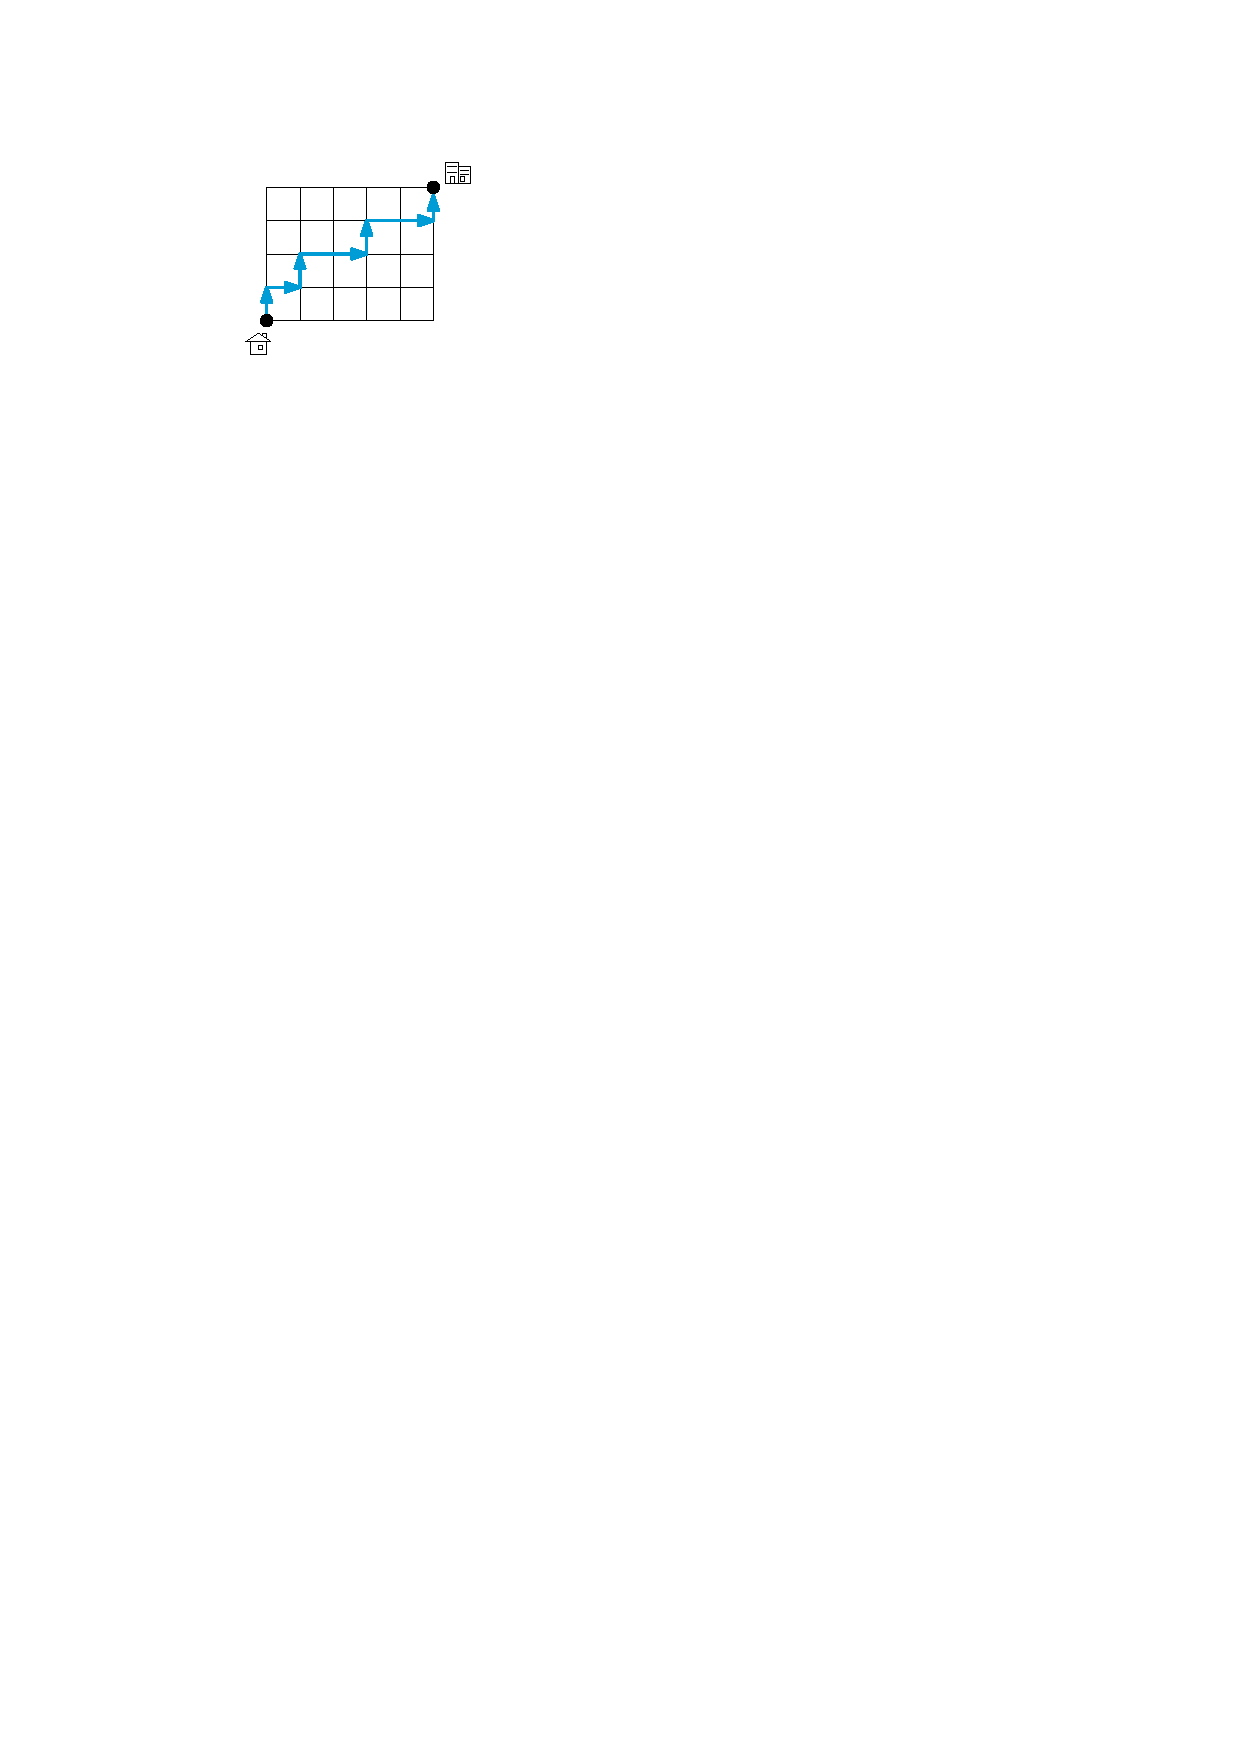
\includegraphics[width=0.3\linewidth]{figures/house-to-bahen-path.pdf}
   \label{fig:home-to-bahen}
\end{figure}

\section{Strings}

\begin{definition}[Binary String]
   A \textit{\textbf{binary string}} of length $n$ is an ordered list of length $n$ of elements from $\{0,1\}$. 
\end{definition}

\begin{example}
   $10011$ is a binary string of length $5$. $\emptyset = \{\}$ is a binary string of length $0$.
\end{example}

Similarly, a \textit{\textbf{ternary string}} of length $n$ is an ordered list of length $n$ of elements from $\{0,1,2\}$.

\begin{definition}[X-String]
   Let $X = \{a_1,\ldots,a_n\}$ be the alphabet. An $X$-string of length $k$ is an ordered list of elements from the set $X$.
\end{definition}

In the previous example, the path from home to Bahen without backtracking can be thought of as an $\{\text{N},\text{E}\}$-strings.

\textbf{Q}: How to relate the set of paths from home to Bahen without backtracking with some set of $\{\text{N},\text{E}\}$-strings? \\
\textbf{A}: Note that not every $\{\text{N},\text{E}\}$-strings can represent a path. In our specific examples, we need exactly walk $5$ blocks east and $4$ blocks north.

\textbf{Q}: How many $\{\text{N},\text{E}\}$-strings of length $9$ are there? \\
\textbf{A}: Let $\mathcal{S} = \{\text{all $\{$N, E$\}$-strings of length 9}\}$. For each $S \in \mathcal{S}$, $S = s_1s_2\ldots s_9$. For each position, there are two choices, N or E. Hence, there are $2^9$ possible $\{\text{N},\text{E}\}$-strings in $\mathcal{S}$.

\begin{theorem}
   For $X = \{a_1,\ldots,a_n\}$, the number of $X$-strings of length $k$ is $n^k$, where $n,k \geq 1$ are natural numbers.
\end{theorem}

\begin{proof}
   Denote $S = s_1\ldots s_k \in \mathcal{S}$. For $s_i$, there are $n$ choices for $i \in \{1, \ldots, k\}$. So there are
   $$
   \underbrace{n \times n \times \cdots \times n}_{\text{$k$ times}} = n^k
   $$
   such strings.
\end{proof}

\begin{definition}[Array]
   An \textit{\textbf{array}} of length $n$ is an ordered list where the elements in position $i$ comes from some alphabet $X_i$.
\end{definition}

\begin{example}
   Ontario health cards have the format: 10 digits of $\{0,1,\ldots,9\}$ followed by two letters from $\mathrm{\{A,\ldots,Z\}}$. There are $(10)^{10} \times (26)^2$ possible health card numbers.
\end{example}

\section{Permutations}

Let $X = \{a_1,\ldots,a_n \}$ be a set of distinct object.

\begin{definition}[Permutation]
   A \textit{\textbf{permutation}} of length $k$ is an $X$-string of length $k$ such that there is no repetition. Equivalently, $s$ is injectively.

   Given integers $n$ and $k$ with $n \geq k$, we let $P(n,k)$ denote the number of permuations of $[n]$ of length $k$.
\end{definition}

\begin{example}
   Suppose $X = \{a,b,c,d\}$. $abc$ is a permutation of length 3. $\emptyset$ is a permutation of length 0. However, $bab$ is not a permutation because of the repeating character $b$.
\end{example}

\begin{remark}
   Because a permutation requires there be no repetition, there is no permutation of length $k$ for $X$ of size $n$ if $k > n$.
\end{remark}

\textbf{Q}: How many permutations of length 4 are there of $X = \{a,b,c,d\}$? \\
\textbf{A}: Let $S = s_1s_2s_3s_4$ be a permutation. There are 4 choices for $s_1$. After choosing $s_1$, there are 3 choices left for $s_2$. After choosing $s_2$, there are 2 choices left for $s_3$. Similarly, after choosing $s_3$, there is 1 choice left for $s_4$. In total, there are $4 \times 3 \times 2 \times 1$ permutations for $\{a,b,c,d\}$.

\begin{definition}[Factorial]
   For any $n \in \N$ such that $n \geq 0$, $n$ \textit{\textbf{factorial}} is defined as
   $$
   n! = n \times (n-1) \times (n-2) \times \cdots \times 2 \times 1
   $$
   In particular, we define $0! = 1$.
\end{definition}

We use $P(n,k)$ to denote the number of permutations of $[n]$ of length $k$ (i.e. $[n] = \{0,1,\ldots,n\}$).

For example, consider the number of permutations of $[3]$.

\textbf{Q}: What are the permutations of length 2 for $[3]$? \\
\textbf{A}: 01, 02, 12, 10, 20, 21

\textbf{Q}: What are the number of permutations of length 3 of $[3]$? \\
\textbf{A}: 012, 021, 102, 120, 210, 201

\textit{Observation}: There are the same number of permutations of $[3]$ of length 3 as the number of permutations of $[3]$ of length 2.

Then, it is natural to ask if we can generalize this. That is, when is $P(n,k)=P(n,k')$?

Consider a permutation of $[3]$ of length 3, $p = p_1p_2$. For $p_1$, there are 3 choices. After choosing $p_1$, there are 2 choices for $p_2$. So, in total, there are $3 \times 2$ permutations of $[3]$ of length 2.

Now, consider a permutation of $[3]$ of length 3, $p = p_1p_2p_3$. For $p_1$, there are 3 choices. After choosing $p_1$, there are 2 choices for $p_2$. After choosing $p_1$ and $p_2$, there is exactly 1 choice for $p_3$. In total, there are $3 \times 2 \times 1$ choices for $p$, a permutation of length $3$ of $[3]$.

\begin{proposition}
   For $n \geq 1$,
   $$
   P(n,n) = P(n,n-1)
   $$
\end{proposition}
\begin{proof}
   The proof is similar to how we showed $P(3,3)=P(3,2)$.
\end{proof}

Next, we ask if there are any other $k=k'$ for some $k,k' \leq n$ and $n\geq 1$ such that $P(n,k) = P(n,k')$.

One common technique in combinatorics is to find a bijective correspondance from one set to another. To show that $P(3,2)=P(3,3)$, we can find a bijective correspondance as shown in the figure below

\begin{figure}[h]
   \centering
   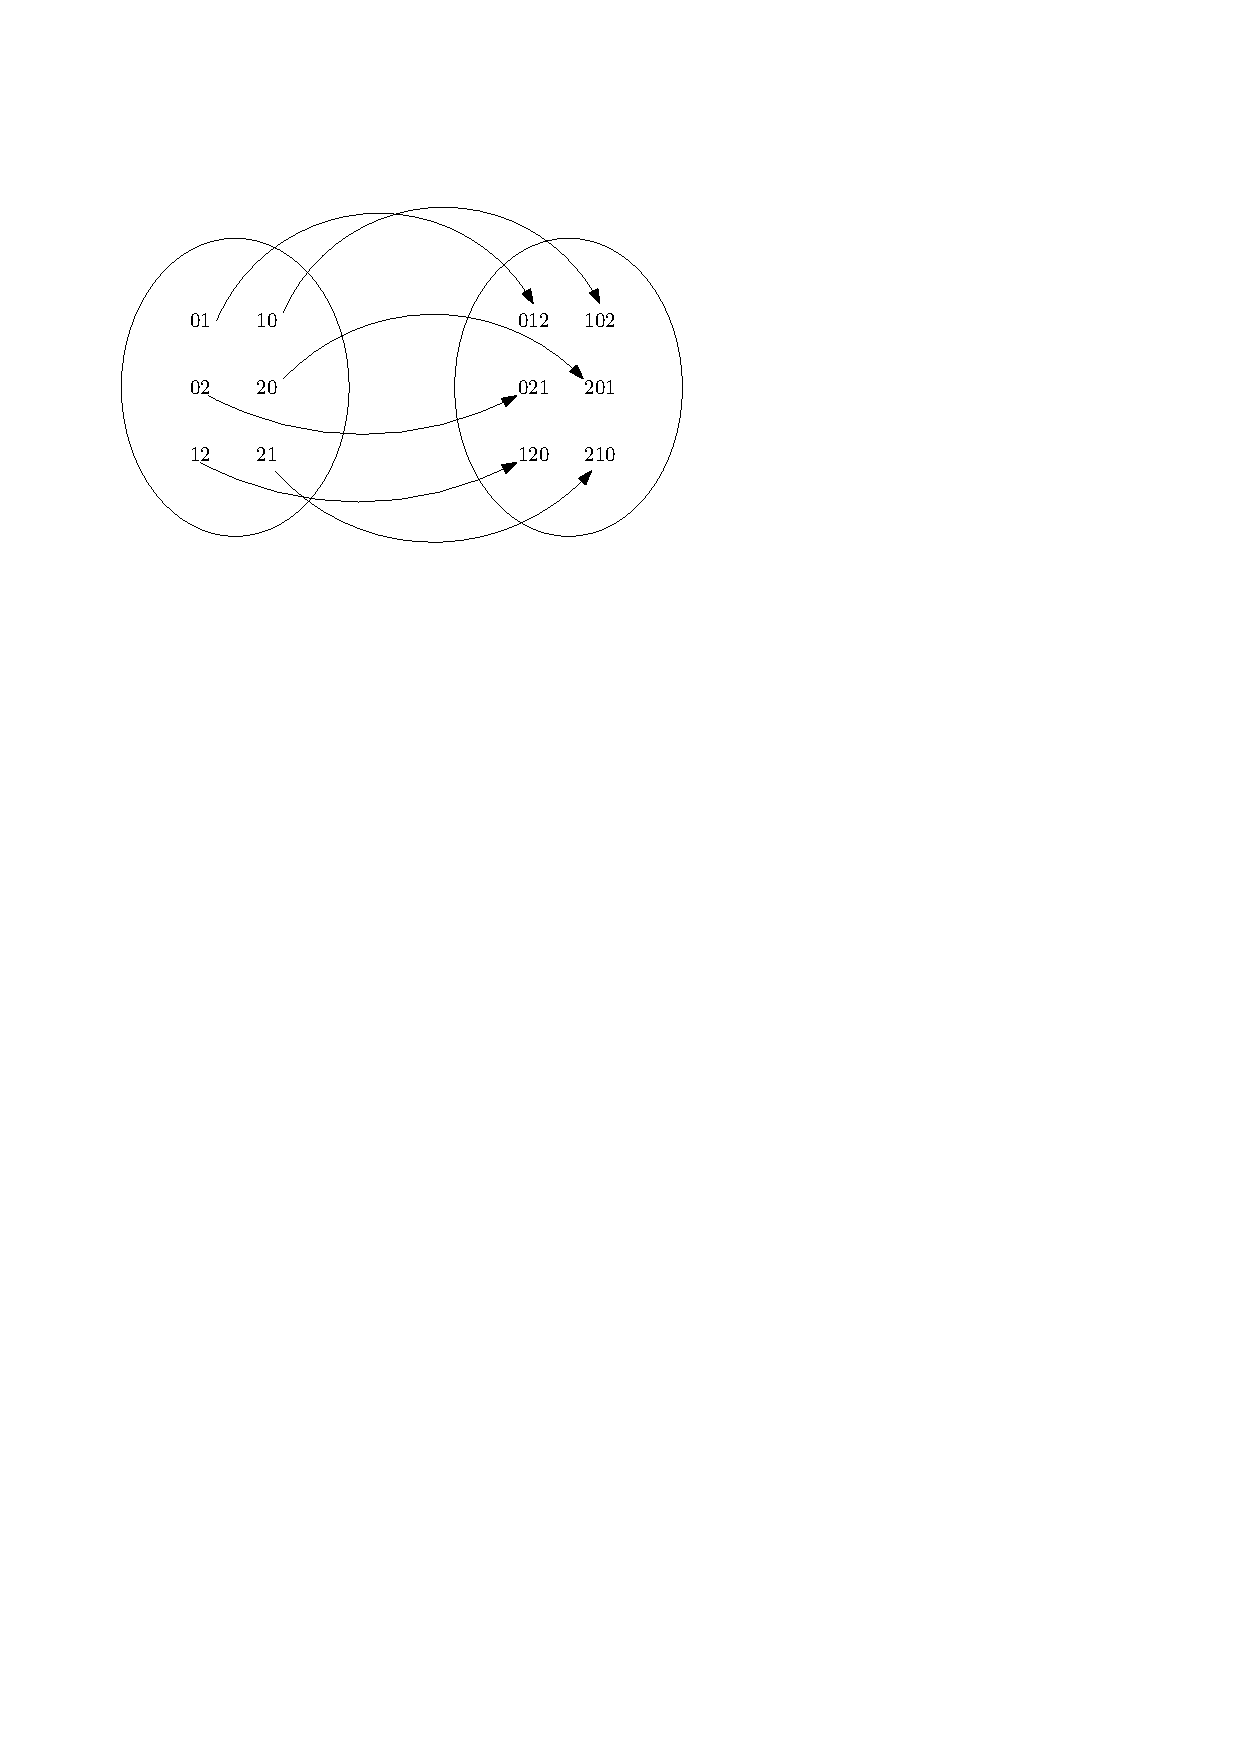
\includegraphics[width=0.4\linewidth]{figures/biject-correspondance.pdf}
   \caption{Bijective correspondance showing $P(3,2)=P(3,3)$.}
\end{figure}

\begin{theorem}
   Given integers $n$ and $k$ with $n \geq k$,
   $$
   P(n,k) = \frac{n!}{(n-k)!}
   $$
\end{theorem}

\begin{proof}
   Consider $p=p_1p_2\cdots p_k$, a permutation of $[n]$ of length $k$. For $p_1$, there are $n$ choices. After choosing $p_1$, there are $n-1$ choices for $p_2$. In general, after choosing $p_i$, there are $n-i$ choices for $p_{i+1}$. We repeat this until we get $p_k$. In total, we have
   $$
   P(n,k) = n \times \cdots \times (n-(k-1)) = \frac{n!}{(n-k)!}
   $$

   Alternatively, we can prove this by fixing $n$ and induct on $k$.
\end{proof}

From this theorem, we get the same result that $P(n,n) = P(n,n-1)$.
\begin{corollary}
   $$
   P(n,n-1) = P(n,n)
   $$
\end{corollary}
\begin{proof}
   $$
   P(n,n) = \frac{n!}{(n-n)!} = n!
   $$
   $$
   P(n,n-1) = \frac{n!}{(n-(n-1))!} = \frac{n!}{1!} = n!
   $$
\end{proof}


\section{Subsets and Combination}

\begin{definition}[Combination]
   Given a set of objects $X$, a combination of size $k$ is a subset $A \subseteq X$ of size $k$.
\end{definition}

\begin{example}
   What are the subsets of $\{1,2,3\}$?
   $$
   \emptyset=\{\}, \{1\}, \{2\}, \{3\}, \{1,2\}, \{1,3\}, \{2,3\}, \{1,2,3\}
   $$
   There are 3 combinations of $\{1,2,3\}$ of size 2.
\end{example}

Set notations:
\begin{multicols}{3}
   $\emptyset$ or $\varnothing$: empty set; \\
   $\in$: element of; \\
   $\subset$: subset of; \\
   $\subseteq$: subset of; \\
   $\subseteq$: proper subset of; \\
   $\not\in$: not an element of
\end{multicols}

\begin{remark}
   For elements of a set, order does not matter.
\end{remark}

Another example
\begin{example}
   Say we have $X=\{a,b,c,d\}$. $\emptyset$ is the unique combination of $X$ of size $0$. $\{a,d\}$ and $\{b,a\}$ are the combinations of $X$ of size 2.
\end{example}

In general, we use the following notation
\begin{definition}
   $C(n,k)$ is the number of combinations of $[n]$ of size $k$ where $0 \leq k \leq k$ are integers.
\end{definition}

\begin{remark}
   Note that as with the case for permutation, there are no combinations of $[n]$ of size $k > n$.
\end{remark}

\textbf{Q}: What is the value of $C(n,k)$? \\
\textbf{A}: Intuitively, there should be more permutations than combinations because order matters for permutations.

Consider the combinations of $[4]$ of size $2$. They are $\{0,1\}, \{0,2\}, \{0,3\}, \{1,2\}, \{1,3\}, \{2,3\}$. So there are 6 combinations. Note that for each combination, we can order it in $2!$ ways, giving us $6 \cdot 2!$ permutations.

\begin{theorem}
   For $n \geq k \geq 0$,
   $$
   C(n,k) = \frac{P(n,k)}{k!}
   $$
\end{theorem}

\begin{proof}
   We will show that for any combination $A$ of $[n]$ of size $k$, there are $k!$ ways to order the elements into permutations of size $k$.

   Note that given a permutation $p = p_1\cdots p_k$, there is exactly one such set $A = \{p_1,\ldots,p_k\}$ because the elements in a permutation do not repeat. Of the $k!$ permutations of $A$, each one is a permutation of $[n]$ of length $k$.

   Hence, there are $C(n,k)$ combinations, and there are $k!$ ways to order each combination such that we get a unique permutation. All such permutations can be obtained this way.

   Therefore, $P(n,k) = C(n,k) \cdot k!$ (the number of permutations is the number of combinations times the number of ways to order each combination), and the theorem follows.
\end{proof}

An alternative notation for $n$ choose $k$ is
$$
C(n,k) = \binom{n}{k} = \frac{n!}{(n-1)!k!}
$$

\begin{corollary}
   $C(n,k) = C(n,n-k)$.
\end{corollary}

\begin{proof}
   Trivially follows from the formula.
\end{proof}

Combinatorially, if we choose $k$ elements of $[n]$ (i.e. tagging them with 1), then the number of ways to tag the ones we chose is the same as the number of ways to tag the ones we did not choose.

\begin{remark}
   $\binom{n}{k}$ are the binomial coefficients. This means the coefficient of $x^k$ in the expansion of $(1+x)^n$ is exactly $\binom{n}{k}$. 
\end{remark}
Intuitively,
$$
\underbrace{(1+x) \cdots \cdots (1+x)}_{\text{$n$ terms}}
$$
for the $x^k$ term, we take $x$ exactly $k$ times and take 1 exactly $n-k$ times.

\section{Applications}

Let us revisit one of the motivating examples at the beginning.

\textbf{Q}: How many ways to get from home to Bahen without backtracking? \\
\textbf{A}: There are 9 steps we need to take. 5 of those 9 steps need to be going to the east, and 4 of the 9 steps need to be going to the north. More formally, we need the number of $\{\text{N,E}\}$-strings of length 9 with 4 N's. This is equivalent to choosing 4 positions/indicies to place the N's or 5 positions/indicies to place the E's. So, in total, we have $\binom{9}{4} = \binom{9}{5}$ paths.

\section{Bijective Correspondance}

Suppose we have sets $A$ and $B$. $f:\;A\to B$ is a function.

\begin{definition}[Injective]
   We say $f$ is injective or one-to-one if $\forall a_1\neq a_2 \in A.\, f(a_1) \neq f(a_2)$.
\end{definition}

\begin{definition}[Surjective]
   We say $f$ is surjective or onto if $\forall b \in B.\, \exists a \in A.\, f(a) = b$.
\end{definition}

\begin{definition}[Bijection]
   We say that $f$ is bijective if $f$ is both injective and surjective.
\end{definition}

\begin{remark}
   If there is a bijective mapping $f:\; A \to B$, then $A$ and $B$ have the same size (cardinality).
\end{remark}

This is useful because it allows us to count things using things that we already know how to count if we can find a bijection between the two sets.

\chapter{Binomial Theorem and Combinatorial Proofs}
\section{Binomial Theorem}

\begin{theorem}[Binomial Theorem]
    For any $x \in \R$, for any $n \geq 0$ natural number
    $$
    (1+x)^n = \sum_{k=0}^n \binom{n}{k} x^k
    $$
\end{theorem}

\begin{proof}
    $$
    \text{LHS} = (1+x)^n = \underbrace{(1+x) (1+x) \cdots (1+x)}_{\text{$n$ times}}
    $$
    When we expand and collect the like terms, we get a polynomial of the form
    $$
    \sum_{k=0}^n c_k x^k = c_0 + c_1x + c_2 x^2 + \cdots + c_n x^n
    $$
    For $k$, the only way to get $x^k$ in the expansion of the LHS is if for $k$ of the $n$ terms in the product to contribute to to $x$, and the rest $n-k$ of the terms to contribute to $1$.

    In total, we have $\binom{n}{k}$ ways to get $x^k$ in the expansions. Hence, $c_k = \binom{n}{k}$.
\end{proof}

The binomial theorem can be equivalently stated as
\begin{theorem}[Binomial Theorem (two variables)]
    For any $x,y \in \R$, $n \in \N$ such that $n \geq 0$,
    $$
    (x+y)^n = \sum_{k=0}^k \binom{n}{k} x^k y^{n-k}
    $$
\end{theorem}

\begin{example}
    $$
    (1+x)^2 = (1 + x)(1 + x) = 1 + \underbrace{x + x}_{\substack{\text{two ways of} \\  \text{picking one 1} \\ \text{and one x}}} + x^2
    $$
    $$
    (1+x)^3 = (1+x) (1+x) (1+x) = 1 + \underbrace{x + x + x}_{\binom{3}{1}x} + \binom{3}{2} x^2 + \binom{3}{3}x^3
    $$
    Choose 3 to be $x$ and other 0 to be 1.
\end{example}

\section{Combinatorial Proofs}

Say you want to prove that
$$
2^n = \sum_{k=0}^n \binom{n}{k}
$$
Combinatorially, the LHS is the number of binary strings of length $n$. The RHS is obtained by summing up the number of binary strings with $k$ 0's in the binary string of length $n$ over all $k = \{0,\ldots,n\}$.

\begin{remark}
    The hard part is making sure you count all cases and are not double counting.
\end{remark}

\begin{example}
    Say we want to prove the identity
    $$
    \binom{2n}{n} = \sum_{k=0}^n \binom{n}{k} \binom{n}{n-k}
    $$
    The LHS can be described as follows. Suppose we have a group of $n$ boys and $n$ girls. In total, we have $2n$ people. Choose $n$ people to form a team.

    For the RHS, we can split into cases where $k$ girls are chosen. For each $k$, there are $\binom{n}{k}$ ways to choose girls and $\binom{n}{n-k}$ ways to choose $n-k$ boys. This summed over all $k \in \{0,\ldots,n\}$ gives us $\sum_{k=0}^n \binom{n}{k} \binom{n}{n-k}$.
\end{example}

\begin{remark}
    Combinatorially, summation often means summing up the counts for each case.
\end{remark}

\subsection{Ideas of a Combinatorial Proof}

Say you want to show an identity with LHS = RHS using a combinatorial proof. We follow these steps
\begin{enumerate}
    \item Come up with a situation to count one side (whichever is easier).
    \item Come up with another way to count the same situation, as described by the harder side.
    \item Show that both count the same objects and conclude that LHS = RHS.
\end{enumerate}

\begin{remark}
    Some hints for writing combinatorial proofs:
    \begin{itemize}
        \item Start with the easier side
        \item Break down the hard side (especially those with summations) into cases based on $k$ and note that sum ($\Sigma$) = ``OR'', product ($\Pi$) = ``AND''
        \item Use facts like $\binom{n}{k} = \binom{n}{n-k}$, $\binom{n}{1} = n$, etc.
        \item There might be information not captured in the algebraic identity
    \end{itemize}
\end{remark}

\begin{example}
    $$
    \sum_{k=1}^n \binom{n}{k} k = n 2^{n-1}
    $$
    for $n \geq 1$.

    For RHS, there are $n$ people and we want to choose 1 to be the captain ($\binom{n}{1}$). Build a team around the captain. For each of the $n-1$ others not chosen, they can be either on the team or not. Thus, $n (2^{n-1})$.

    For LHS, we split into cases based on there being $k$ people on the team. First, choose $k$ of the $n$ people to be on the team. From the $k$ people, we choose 1 to be the captain ($\binom{k}{1}$). Summing this for all $k \in \{1,\ldots,n\}$ gives the number of all possible configuraitons to form a team with at least one captain.
\end{example}

\section{More on Combinatorial Proofs}

\begin{example}
    Prove
    $$
    \binom{n}{k} = \binom{n - 1}{k - 1} + \binom{n - 1}{k}
    $$
    for $n \geq k \geq 1$.

    For LHS, there are $n$ people named $1, \ldots, n$. Choose $k$ of them.

    For RHS, we fix one person. There are 2 cases: (1) Person 1 is included as part of the $k$ people. We have $n-1$ people left, and we need to choose $k-1$ people; (2) Person 1 is not included as part of the $k$ people. There are $n-1$ people left, of which we need to choose $k$ people.

    So in total, we have $\binom{n-1}{k-1} + \binom{n-1}{k}$ ways of choosing $k$ people from $n$ people.
\end{example}

For the previous example, we can also give a non-combinatorial proof. Observe that $\binom{n}{k}$ is the value at the $n$th row and $k$th column of the Pascal's triangle. Similarly, $\binom{n-1}{k-1}$ and $\binom{n-1}{k}$ are the entries at position $(n-1,k-1)$ and $(n-1,k)$ in the Pascal's triangle, whose sum is equal to the $(n,k)$ entry.

\begin{example}
    Prove
    $$
    \binom{2n}{2} = 2 \binom{n}{2} + n^2
    $$
    for $n \geq 2$.

    For LHS, consider the situation where we have $n$ girls and $n$ boys. Choose 2 of them to form a team.

    For RHS, there are 2 cases: \\
    \textbf{Case 1}: Both are the same gender. There are 2 choices for the gender, and for each gender, there are $\binom{n}{2}$ ways to choose 2 people. \\
    \textbf{Case 2}: They have different genders, in which case we choose $1$ from $n$ boys and $1$ from $n$ girls.

    In total, we have $2 \binom{n}{2} + n^2$ for the RHS.
\end{example}

\textbf{Exercise 1}: Prove that
$$
\binom{4n}{2n} = \sum_{k=0}^n \binom{2n}{k} \binom{2n-k}{2n-2k} 2^{2n-2k}
$$
for $n \geq k \geq 1$.

\textbf{Exercise 2}: Prove that
$$
\sum_{k=0}^n \binom{2n}{k}^2 = \frac{\binom{4n}{2n} + \binom{2n}{n}^2}{2}
$$
for $n \geq 1$.

\section{Binomial Coefficients}

Suppose Alice, Bod, and Carol are sharing 10 identical cookies. How many ways are there of sharing the cookies such that they each get some $n$ number of cookies (where $n$ is some natural number including 0).

We cannot use the old method of choosing number of cookies each person get because this leads to double counting.

Instead, let us put bars/dividers that partition the cookies into 3 partitions. There are $10 + 2$ positions, and we need to put 2 \textbf{identical dividers}. The dividers can be anywhere.

\begin{figure}[htbp]
    \centering
    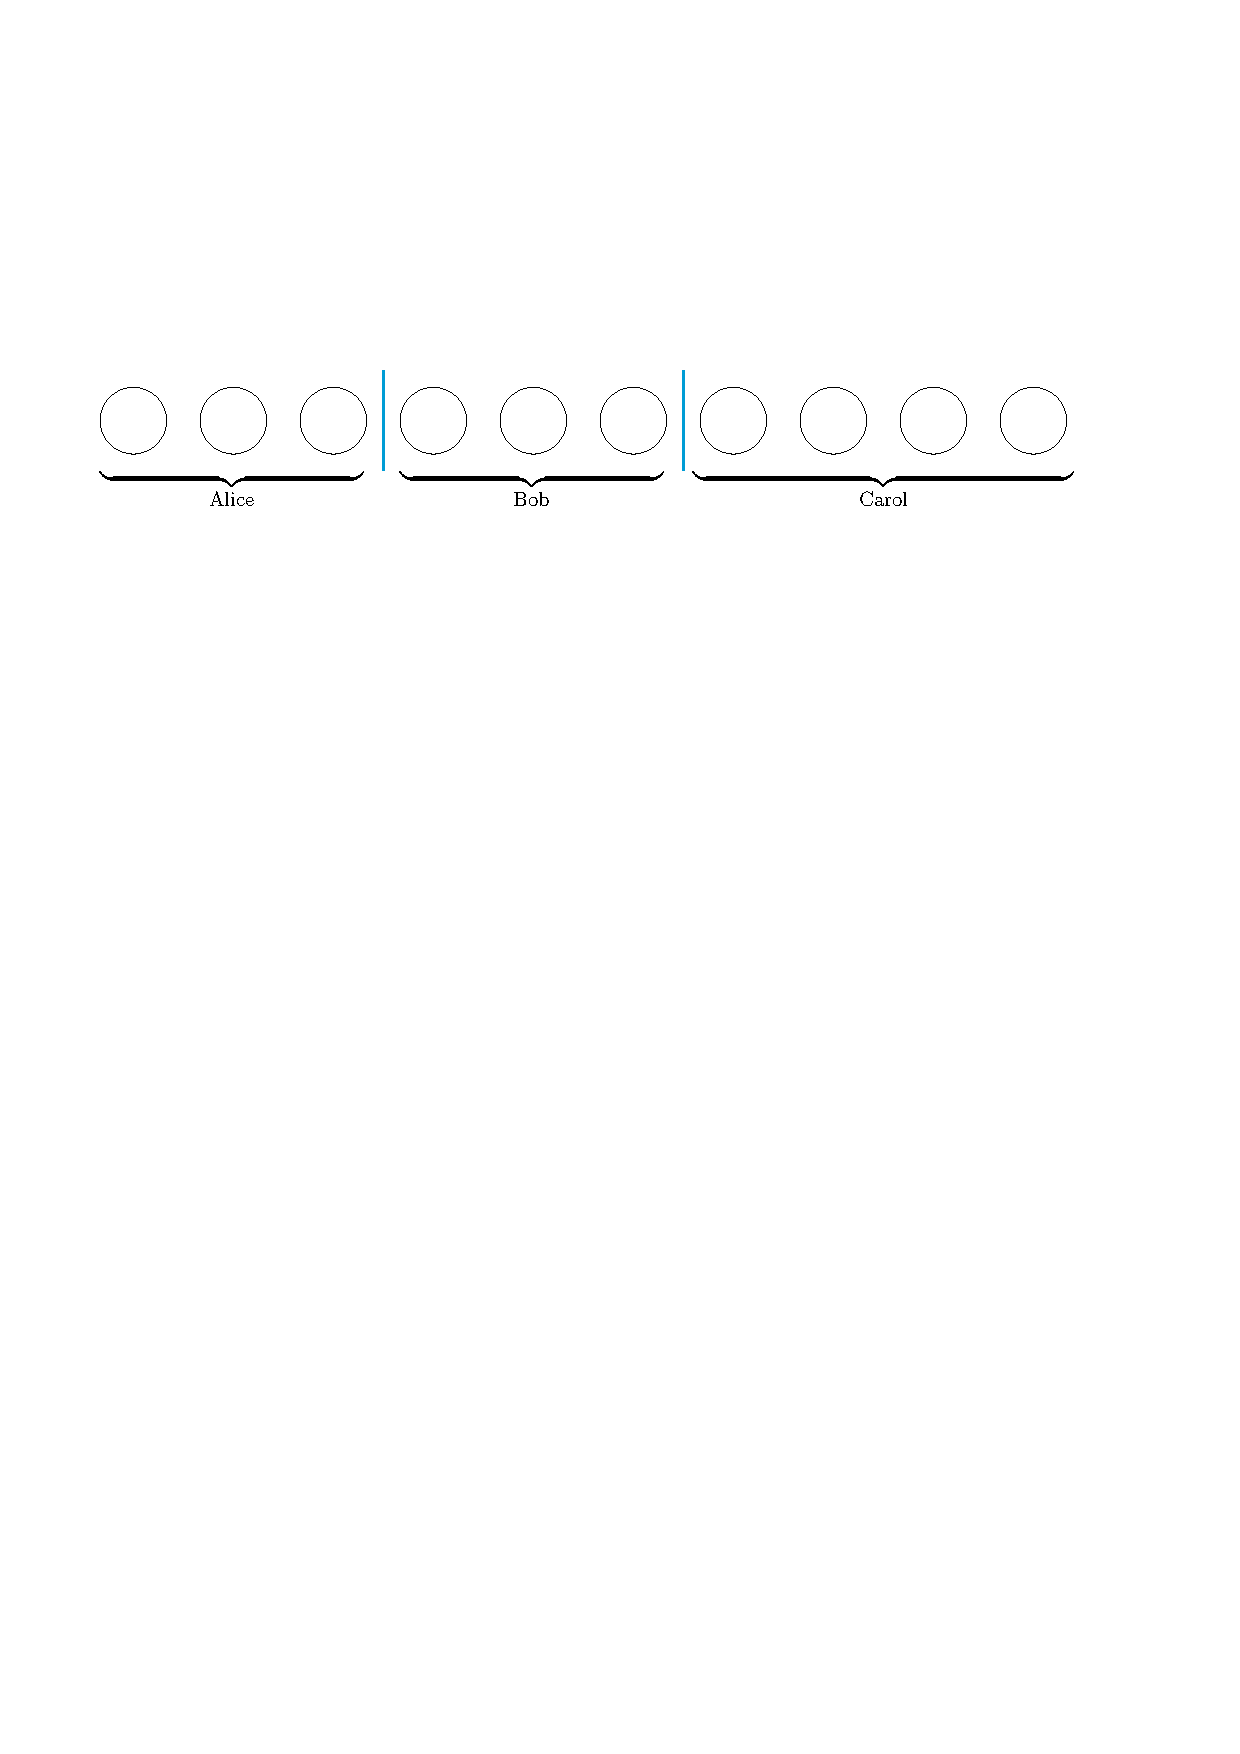
\includegraphics[width=.6\linewidth]{figures/cookie-distribution.pdf}
    \caption{Placing bars to partition the cookies.}
    \label{fig:cookie-distribution}
\end{figure}

In general, if there are $n$ identical items to be shared between $k \leq n$ people, then there are $\binom{n+(k-1)}{k-1}$ configurations. This method is known as the ``stars and bars'' method.

The cookie distribution example is equivalent to the question of asking how many integer solutions there are to the equation $x_1 + x_2 + x_3 = 10$, with the constraint $x_1,x_2,x_3 \geq 0$.

\textbf{Q}: Now, let us consider a variation of our pervious example. What if now we add the new constraint that \textbf{Alice and Bod each get at least 1 cookie}. \\
\textbf{A}: There are many ways to solve this modified example. One general way is to use \textit{\textbf{inclusion-exclusion}}. We eliminate cases where Alice gets 0 cookies and Bod gets 0 cookies. Then, add back the case where neither Alice nor Bob get cookies.

Alternatively, we can first distribution 2 cookies to Alice and Bob. For the remaining 8 cookies, we can distribute them as before.

\textbf{Q}: What if they can have cookies leftover? \\
\textbf{A}: Sum over all cases where they distribute $k$ cookies where $0 \leq k \leq 10$. Another easier way is to have ``\textbf{Charity}'' be the 4th person, so this is the number of ways 4 people are distributing 10 cookies. From this, we get
$$
\sum_{k=0}^{10} \binom{k+2}{2} = \binom{10 + 3}{3}
$$

\textbf{Q}: What if Alice wants at most 4 cookies? \\
\textbf{A}: Sum over cases where Alice gets $k$ cookies for $0 \leq k \leq 4$. Alternatively, subtract the number ways where Alice gets more than 4 cookies.

\begin{remark}
    For the previous example, we cannot assign 6 cookies to Bob and Carol and then distribute the rest 4. This results in double counting. Consider the following situations:
    \begin{itemize}
        \item Initially, give 3 cookies to Bob, 3 to Carol. Then give all 4 cookies to Bob.
        \item Initially, give 6 cookies to Bob, 0 to Carol. Then, give 1 to Bob and 3 to Carol.
    \end{itemize}
    Note that in both of these two situations, Alice, Bob, and Carol end up getting the same number of cookies. But the number of ways is counted twice.

    In combinatorics, it is always important to make sure that we don't overcount.
\end{remark}

\section{Lattice}

Recall the motivating example in the first lecture where we considered the ways to go from home to Bahen. We now generalize the problem into one concerning \textit{\textbf{lattice paths}}.

\begin{definition}[Lattice]
    An $m \times n$ grid between the coordinates $(0,0)$ and $(m,n)$ is called a \textit{\textbf{lattice}}.
\end{definition}

\begin{definition}[Lattice Path]
    A \textit{\textbf{lattice path}} for an $m \times n$ lattice between $(0,0)$ and $(m,n)$ is a sequence of ordered pairs of integers $(a_0,b_0),(a_1,b_1),\ldots,(a_t,b_t)$ such that for each $i$, $1 \leq i \leq t-1$ and either $(a_{i+1},b_{i+1}) = (a_i + 1, b_i)$ or $(a_{i+1},b_{i+1}) = (a_i, b_i + 1)$ (i.e. we can only move north or east by exactly one each step).
\end{definition}

A lattice path of length $t$ can be represented equivalently using a binary string of length $t-1$ over the alphabet $\{\mathrm{N,E}\}$.

\textbf{Q}: If we have a square lattice from $(0,0)$ to $(n,n)$, how many lattice paths from $(0,0)$ to $(n,n)$ do not go above the line $x=y$?

\begin{figure}[htbp]
    \centering
    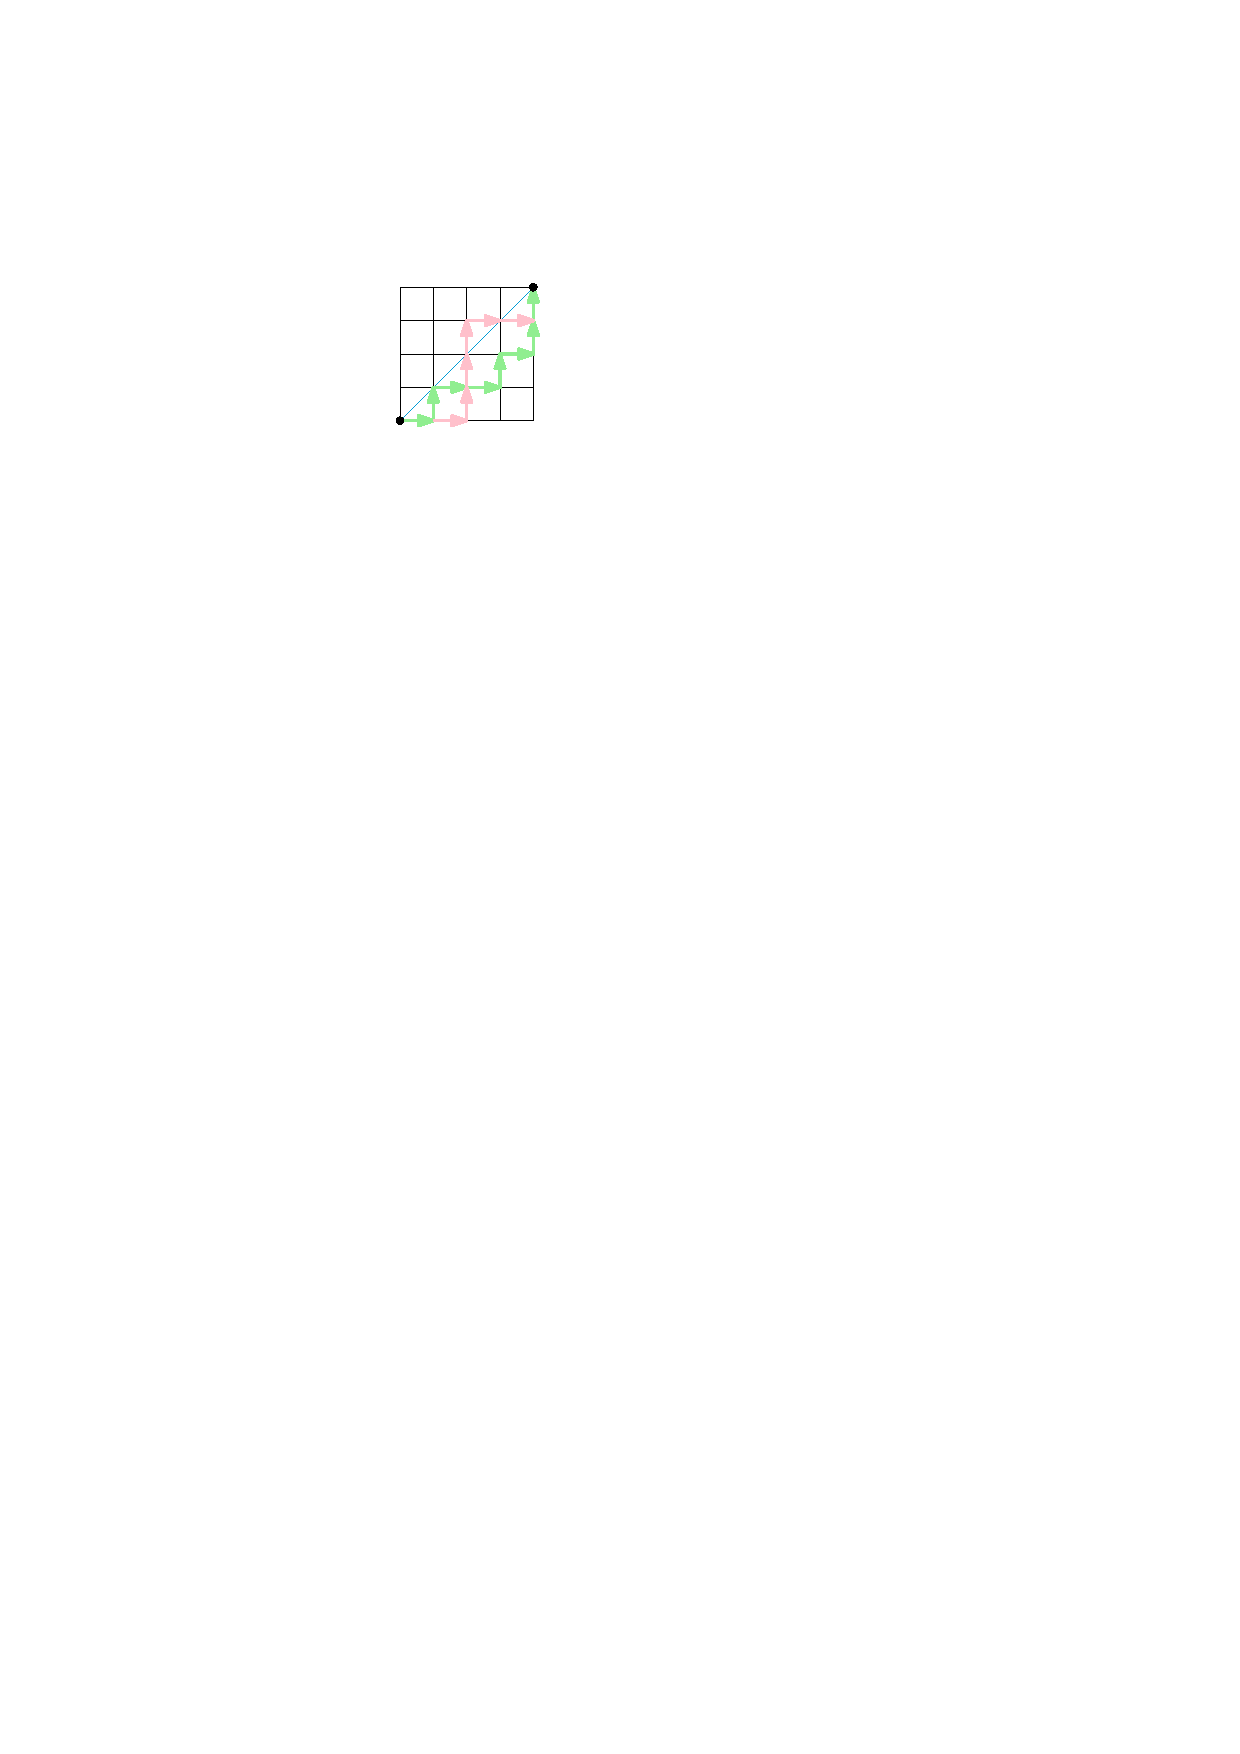
\includegraphics[width=.2\linewidth]{figures/dyck-path.pdf}
    \caption{The green path is a valid Dyck path whereas the red path is not.}
    \label{fig:dyck-path}
\end{figure}

\begin{definition}[Dyck Path]
    Lattice paths from $(0,0)$ to $(n,n)$ that do not go above the diagonal line $x=y$ are called \textit{\textbf{Dyck paths}} of length $2n$.
\end{definition}

Then, the $\{(,)\}$-string (string over the alphabet containing left and right parentheses, where ``('' corresponds to East, ``)'' corresponds to North) of length $2n$ that correspond to Dyck paths are exactly the strings where we do not have more ``)'' then ``('' as we read it from the left. Therefore, determining if a path is a Dyck path is equivalent to checking for \textbf{balanced parenthesis}.

We define the following notations
$$
\mathcal{L}_{(m,n)} = \{ \text{lattice paths from $(0,0)$ to $(n,n)$} \}
$$
and
$$
\mathcal{D}_{n} = \{ \text{Dyck paths of length $2n$} \}
$$

\begin{definition}[Catalan Number]
    The number of Dyck paths of length $2n$ is $C(n)$. $C(n)$ is called the $n$th \textit{\textbf{Catalan number}}.
\end{definition}

\begin{theorem}
    $$
    C(n) = \binom{2n}{n} - \binom{2n}{n-1}
    $$
\end{theorem}

\begin{remark}
    $$
    \begin{aligned}
        \binom{2n}{n} - \binom{2n}{n-1} &= \frac{(2n)(2n-1)\cdots (n+1)}{n(n-1)\cdots (1)} - \frac{(2n) \cdots (n+2)}{(n-1) \cdots (1)} \\
        &= \frac{(2n)(2n-1)\cdots (n+1)}{n(n-1)\cdots (1)} - \frac{(2n) \cdots (n+2){\color{red} n(n+1)}}{(n-1) \cdots (1) {\color{red} n(n+1)}} \\
        &= \frac{(2n)(2n-1) \cdots (n+1)}{(n)(n-1) \cdots (1)} \left[ 1 - \frac{n}{n+1} \right] \\
        &= \binom{2n}{n} \frac{1}{n+1}
    \end{aligned}
    $$
\end{remark}

\begin{proof}
    Let
    $$
    \mathcal{B}_{n} = \{ \text{lattice paths from $(0,0)$ to $(n,n)$ that go above $x=y$} \}
    $$
    be the set of non-Dyck paths. Then, $\mathcal{L}_{(n,n)} \setminus \mathcal{B}_n = \mathcal{D}_n$.

    Since $\mathcal{B}_n$ is a finite set, $|\mathcal{L}_{(m,n)} \setminus \mathcal{B}_n| = |\mathcal{L}_{(n,n)}| - |\mathcal{B}_n|$. We already know that $|\mathcal{L}_{(n,n)}| = \binom{2n}{n}$. This is from choosing $n$ positions to go North or $2n-n$ positions to go East.

    For $|\mathcal{B}_n|$, we would like to consider how to transform a ``bad'' lattice path into one that goes $n-1$ units E and $n+1$ units N. For a bad path, since it goes above the diagonal, there must be a first time it goes above $x=y$.

    Let $s = s_1s_2\ldots s_{2n}$ be a bad path. We claim that the first step when $s_i$ goes above $x=y$ is at an odd index $i$. This is because immediately before we crossed the line, we were on the line at index $i-1$ with $x=y$. At that point, we must have taken the same number of steps East as North. Up until $s_i$, we have used 1 more N than E. After $s_i$, there is one less N than E in the remaining steps.

    Consider the transformation 
    $$
    s_1s_2s_3\ldots s_i s_{i+1} \ldots s_{2n} \to s_1s_2s_3 \ldots s_i \overline{s_{i+1}} \ldots \overline{s_{2n}}
    $$
    We observe that this new path is a lattice path from $(0,0)$ to $(n-1,n+1)$. For that, there are $\binom{2n}{n-1}$ possible paths.

    Pictorially, we flip the steps after the $i$th move as shown in the figure below.

    \begin{figure}[htbp]
        \centering
        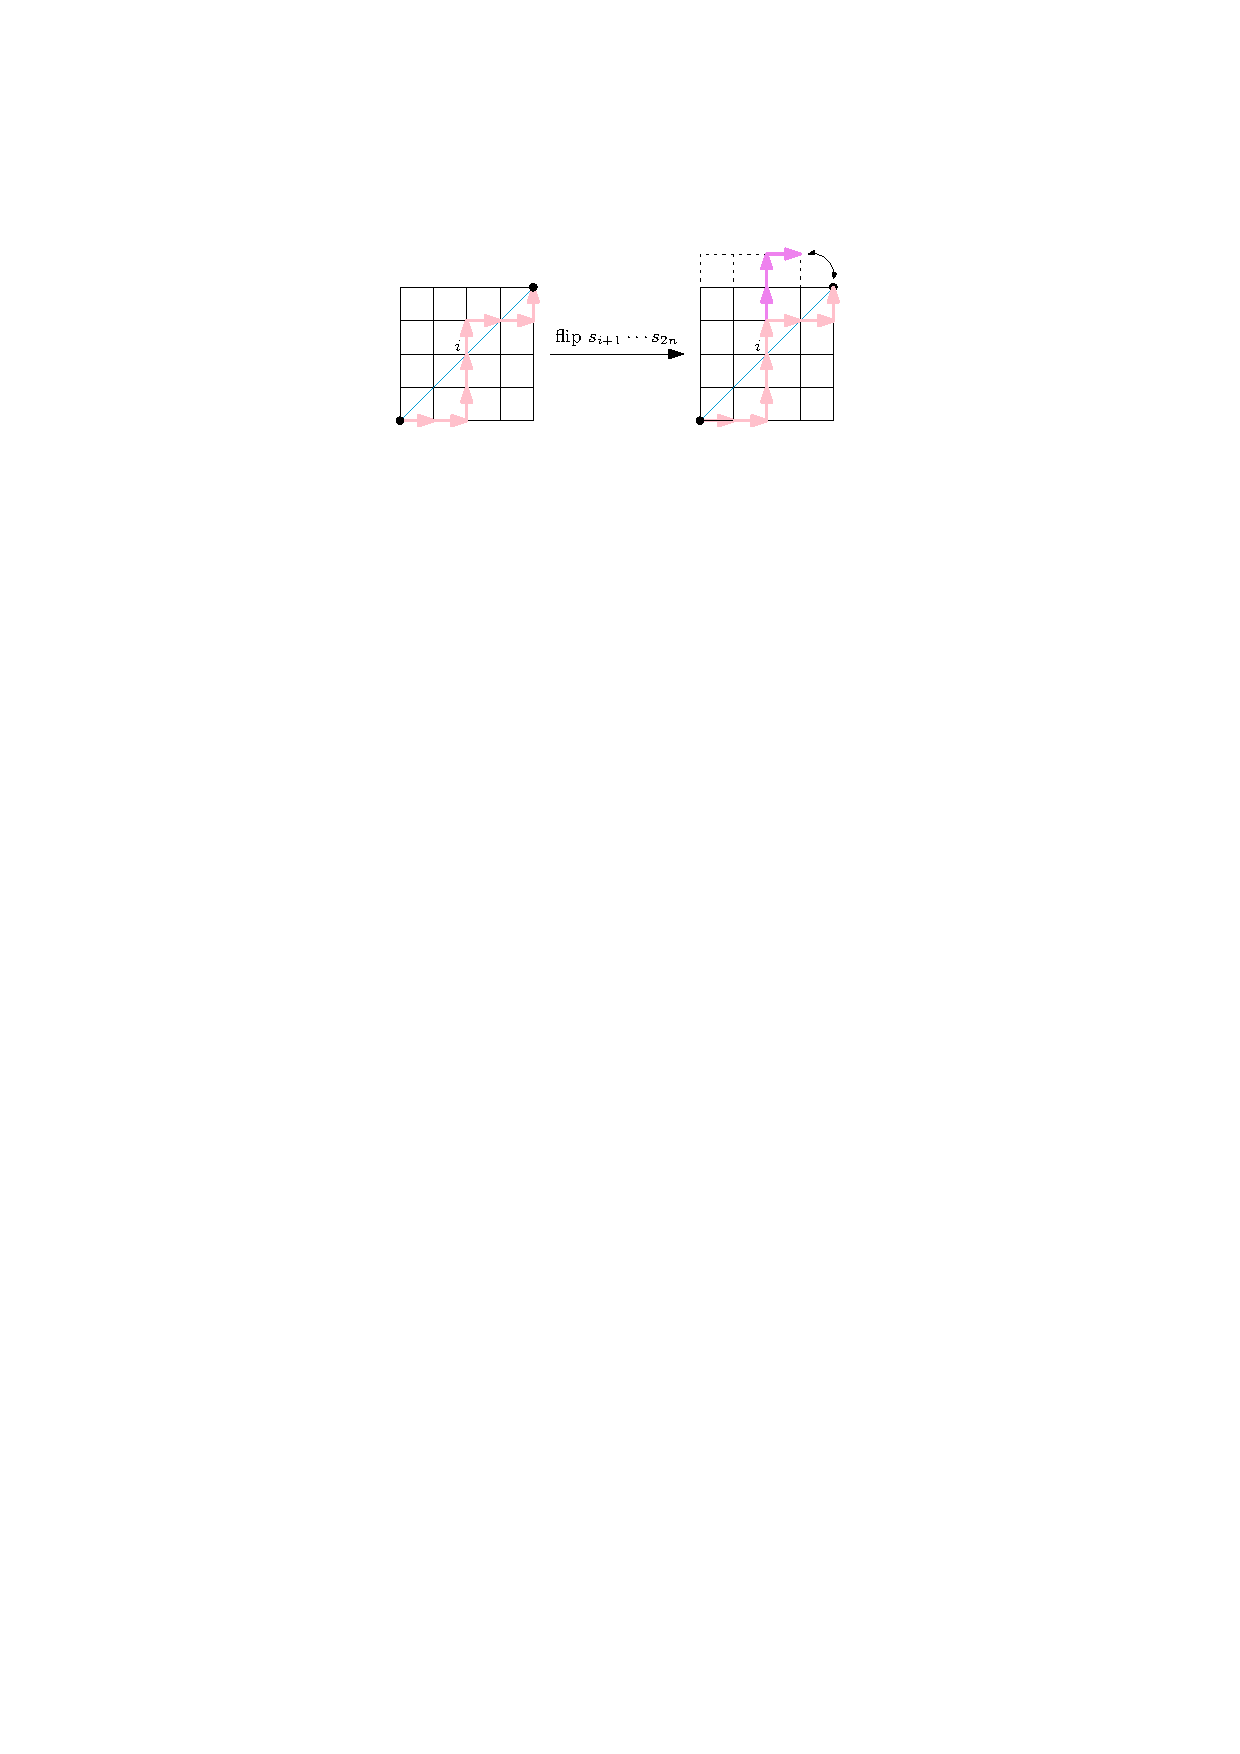
\includegraphics[width=0.5\linewidth]{figures/catalan-number-proof.pdf}
        \caption{Converting a non-Dyck path from $(0,0)$ to $(n,n)$ that goes above $x=y$ into a path in an $n-1 \times n+1$ lattice.}
        \label{fig:catalan-number-proof}
    \end{figure}
\end{proof}

\chapter{The Pigeonhole Principle}
\section{The Pigeonhole Principle}

\begin{theorem}[The Pigeonhole Principle]
    Let $X$ be a set of $n$ objects. Suppose $\{X_1,\ldots,X_k\}$ from a partition of $X$ (i.e. a family of disjoint sets whose union is $X$). If $k < n$, then $\exists i \in \{1,\ldots,k\}$ such that $|X_i| \geq 2$.
\end{theorem}

\begin{proof}
    Suppose for contradiction that for all $i \in \{1,\ldots,k\}$, $|X_i| = 1$. Since $\{X_1,\ldots,X_k\}$ is a partition, 
    $$
    n = |X| = \sum_{i=1}^k |X_i| = k.
    $$
    But this is contradiction since $k < n$.
\end{proof}

Alternatively, we can state the Pigeonhole Principle in terms of a mapping function.

\begin{theorem}[The Pigeonhole Principle]
    Let $X$ be a set of $n$ objects. Let $s:\; X \to \{1,\ldots,k\}$. If $k < n$, then $s$ cannot be injective. That is, there exist distinct $x,y \in X$ such that $s(x) = s(y)$.
\end{theorem}

\begin{proof}
    For $i \in \{1,\ldots,k\}$, let $X_i = \{x \in X \mid s(x) = i\}$. Suppose for contradiction that $s$ is injective. Then, it follows that $X_i$ are disjoint and 
    $$
    \bigcup_{i=1}^k X_i = X.
    $$
    But again, since $s$ is injective $|X_i| \leq 1$ for all $i \in \{1,\ldots,k\}$ and this is a contradiction since $k < n$.
\end{proof}

\section{Generalized Pigeonhole Principle}

\section{Applications of the Pigeonhole Principle}

\subsection{Ramsey Theory}

\part{Induction and Recurrence}

\chapter{Induction}
\section{Induction}

\begin{definition}
    A mathematical statement or a \textit{\textbf{statement}} is a sentence or expression which can be true or false.
\end{definition}

1 + 1 = 2 is a statement, but 1 + 1 is not a statement. An open statement is a statement that depends on some variables.

\subsection{Principle of Induction}

Note that in this course, $\N = \{1,2,\ldots\}$.

\textbf{Principle of Weak Induction}: Suppose we have a family of statements $P(n)$ for all $n \in \N$, and suppose the following holds:
\begin{enumerate}
    \item $P(1)$ holds, and
    \item if $P(k)$ holds, then $P(k+1)$ holds.
\end{enumerate}
Then, we can conclude $P(n)$ is true for all $n \in \N$.

\begin{remark}
    The base case does not have to be for $n=1$ if we are not proving the statement for all $n \in \N$. Say, for example, that we want to show $P(n)$ holds for all $n \in \N$ such that $n \geq 5$. Then, we can use $P(5)$ as the base case.
\end{remark}

For example, suppose we want to show $\forall n \in \N.\, \sum_{i=0}^n 2^i = 2^{n+1} - 1$.

\begin{proof}
    Let $P(n)$ be the statement
    $$
    ``\sum_{i=0}^{n}2^i = 2^{n+1} - 1"
    $$
    \textbf{1. Base Case}: When $n=1$, LHS = $\sum_{i=0}^n 2^i = 2^0 + 2^1 = 3$. RHS = $2^{i+1} - 1 = 3$. LHS = RHS, so $P(1)$ holds.
    
    \textbf{2. Inductive Case}: Assume $P(k)$ holds (inductive hypothesis). WTS $P(k+1)$ holds. The LHS of $P(k+1)$ is
    $$
    \text{LHS} = \sum_{i=0}^{k+1} 2^i = \underbrace{\sum_{i=0}^k 2^i}_{\substack{\text{LHS of $P(k)$} \\ \text{by IH, equals} \\ \text{RHS of $P(k)$}}} + 2^{k+1} = (2^{k+1} - 1) + 2^{k+1} = 2\cdot 2^{k+1} - 1 = 2^{k+2} - 1
    $$
    which is equal to RHS of $P(k+1)$.

    Since we have (1) and (2), by the Principle of Induction, we can conclude that $P(n)$ holds for all $n \in \N$.
\end{proof}

\subsection{Strong Induction}

\textbf{Principle of Strong Induction}: Suppose we have a family of statements $P(n)$ for all $n \in \N$. Suppose the following are true:
\begin{enumerate}
    \item $P(1)$ is true, and
    \item if $P(m)$ is true for all $1 \leq m \leq k$, then $P(k+1)$ is true.
\end{enumerate}
Then, we can conclude $P(n)$ is true for all $n \in \N$.

Suppose we want to show the Fundamental Theorem of Arithmetics (without the uniqueness part), which states that for all $n \in \N$ such that $n \geq 2$, $n$ is a product of primes.

\begin{proof}
    Let $P(n)$ be that $P(n)$ = ``$n$ is a product of primes''.

    \textbf{1. Base Case}: $P(2)$. Since 2 is a prime, it is a product of primes.

    \textbf{2. Inductive Case}: Suppose that for all $m$ such that $2 \leq m \leq k$, $P(m)$ holds. WTS $P(k+1)$ holds. If $k+1$ is prime, then $P(k+1)$ trivially holds. Otherwise, $k+1$ is composite, so there exists $a,b \in \N$ with $2 \leq a,b < k+1$ such that $k+1 = ab$. So since $P(a)$ and $P(b)$ hold by inductive hypothesis, $a$ and $b$ are both products of primes. So $k+1 = ab$ is a product of primes, so $P(k+1)$ holds.
\end{proof}

\section{Recursion}

As an example, consider the Catalan numbers $C_n = \frac{1}{n+1} \binom{2n}{n}$ for $n \geq 0$. Note that $C_0 = 1$ because of the empty path and $C_1 = 1$. Prove the recursive identity
$$
C_{n+1} = \sum_{i=1}^{n+1} C_{i-1} C_{n+1-i}
$$
for $n \geq 0$.

\begin{proof}
    Let $p = p_1p_2\ldots p_{2n}$ be a Dyck path of length $2n$. Let $p_1\ldots p_{2i}$ be the segment of $p$ up until the first time it touches $x=y$ (but not crosses). So, $p_1=$ E and $p_{2i}=$ N. $p_i$ cannot go North because otherwise we would cross the diagonal. For a similar reason, $p_{2i}$ must go North.

    Then, $p_2\ldots p_{2i-1}$ is a Dyck path of length $2(i-1)$. We can split into cases based on the first time after $(0,0)$ where the path touches the diagonal. It can be at $i = 1,\ldots,n+1$. At a given $i$, we break into two Dyck paths: $p_2 \ldots p_{2i-1}$ of length $2(i-1)$ and $p_{2i+1}\ldots p_{2(n+1)}$ of length $2(n+1-i)$. The first path have $C_{i-1}$ possibilities, and the second path have $C_{n+1-i}$ possibilities.

    In total, we have $\sum_{i=i}^{n+1} C_{i-1} C_{n+1-i}$ number of Dyck paths of length $n+1$.
\end{proof}

\begin{definition}
    Let $\{a_n\}_{n\geq 1}$ be a sequence of real numbers. We say that this sequence satisfies a \textit{\textbf{recurrence relation}} if we can define the $n$th term based on the terms that come before it.
\end{definition}

What we proved just now is a recurrence formula for the Catalan numbers. Namely,
$$
C_{n+1} = \sum_{i=1}^{n+1} C_{i-1} C_{n+1-i}
$$
is a recurrence relation on $\{C_n\}_{n\geq 0}$ with $C_0 = 1$.

\subsection{Proving Recurrences}

Consider the Fibonacci numbers with $F_1 = 1$ and $F_2 = 1$, given by the recurrence relation
$$
F_n = F_{n-1} + F_{n-2} \qquad n \geq 3
$$

Induction is a method of proving statements. Recursion is a way of defining/giving a formula for some quantities.

\begin{example}
    We have a closed form expression of $F_n$. Let $\varphi = \frac{1+\sqrt{5}}{2} \approx 1.6$, and let $\psi = \frac{1-\sqrt{5}}{2}$ be the conjugate of $\varphi$. These are the roots of $x^2 = x + 1$. We would like to show that
    $$
    F_n = \frac{\varphi^{n} - \psi^{n}}{\sqrt{5}}
    $$ 
    for all $n \geq 1$.
\end{example}

We prove this closed form formula using induction.

\begin{proof}
    Let $P(n)$ be the statement we want to prove.

    1. Base Case: $P(1)$. LHS $= F_1 = 1$. RHS $= \frac{\varphi^2 - \psi^2}{\sqrt{5}} = \frac{\left( \frac{1+\sqrt{5}}{2}\right) - \left( \frac{1-\sqrt{5}}{2} \right)}{\sqrt{5}} = \frac{2 \frac{\sqrt{5}}{2}}{\sqrt{5}} = 1$.

    2. Base Case: $P(2)$. LHS = $F_2 = 1$. RHS = $\frac{\varphi^2 - \psi^2}{\sqrt{5}} = \frac{\varphi - \psi}{\sqrt{5}} = 1$.

    3. Inductive Case: Assume $P(n)$ holds for all $1 \leq m \leq k$. WTS $P(k+1)$ holds. Consider the LHS of $P(k+1)$. We have
    $$
    F_{k+1} = F_k + F_{k-1} = \frac{\varphi^k - \psi^k}{\sqrt{5}} + \frac{\varphi^{k-1} - \psi^{k-1}}{\sqrt{5}}
    $$
    by IH. Collect like terms
    $$
    \text{LHS} = \frac{\varphi^{k-1} (\varphi + 1) - \psi^{k-1}(\psi + 1)}{\sqrt{5}} = \frac{\varphi^{k-1}(\varphi^2) - \psi^{k-1}(\psi^2)}{\sqrt{5}}
    $$
    since $\varphi$ and $\psi$ are the solutions to $x^2 = x + 1$. This implies that
    $$
    \text{LHS} = \frac{\varphi^{k+1} - \psi^{k+1}}{\sqrt{5}} = \text{RHS}
    $$
    So $P(k+1)$ holds.
\end{proof}

\begin{remark}
    If instead, we prove the statement
    $$
    P(n) = ``F_n = \frac{\varphi^n - \psi^n}{\sqrt{5}} \land F_{n+1} = \frac{\varphi^{n+1}-\psi^{n+1}}{\sqrt{5}}"
    $$
    We can, in fact, use weak induction.
\end{remark}

Let $a_n$ be the max number of intersections of $n$ lines in the plane. Find a recurrence relation for $a_n$. $a_0 = 0$, $a_1 = 0$, $a_2 = 1$, and $a_3 = 3$. Note that two lines intersect unless parallel. Any two parallel lines can be nudged slightly to not be parallel. Moreover, if 3 lines intersect at a point, we can nudge them so they intersect at distinct pairwise intersections. If we know $a_n$, we can have $a_{n+1} = a_n + n$.

\chapter{Generating Functions}
\section{Ordinary Generating Function}

\begin{definition}[Ordinary Generating Function]
    Given a sequence of real numbers $a_n$ for $n \geq 0$, we call the function
    $$
    F(x) = \sum_{n=0}^\infty a_n x^n
    $$
    the \textbf{ordinary generating function} associated to $a_n$.
\end{definition}

The above may not be convergent for any $x$ although often in combinatorics, it will be convergent for many $x$. We mainly use these functions as a bookkeeping system. Generating function is a useful tool to analyze the behavior of sequences.

\subsection{Geometric Series}

\begin{theorem}
    Consider the sequence $a_n = 1$ for all integers $n \geq 0$. The associated generating function is $F(x) = \frac{1}{1-x}$.
\end{theorem}

\begin{proof}
    It suffices to show that $(1-x) F(x) = 1$. Consider the expansion of this expression:
    $$
    \begin{aligned}
        (1-x) F(x) &= (1-x) \sum_{n=0}^\infty x^n \\
        &= \sum_{n=0}^\infty x^n - x \sum_{n=0}^\infty x^n \\
        &= \sum_{n=0}^\infty x^n - \sum_{n=0}^\infty x^{n+1} \\
        &= 1
    \end{aligned}
    $$
\end{proof}

Next, we consider the \textbf{finite geometric series}.

\begin{theorem}
    Consider the sequence $a_n = 1$ for all integers $0 \leq n \leq k$ and $a_n = 0$ when $k > n$. The associated generating function is $F(x) = \frac{1-x^{k+1}}{1-x}$
\end{theorem}

\begin{proof}
    $$
    \begin{aligned}
        (1-x)F(x) &= (1-x) \sum_{n=0}^k x^n \\
        &= \sum_{n=0}^k x^n - \sum_{n=0}^k x^{n+1} \\
        &= x^0 - x^{k+1}
    \end{aligned}
    $$
\end{proof}

\subsection{Some Other Examples}

\begin{example}
    Compute the generating function for the following $a_n$:
    \begin{itemize}
        \item $a_n = 2$ for all $n \geq 0$: $F(x) = \sum_{n=0}^\infty 2 x^n = \frac{2}{1-x}$.
        \item $a_n = 2^n$ for all $n \geq 0$: $F(x) = \sum_{n=0}^\infty 2^n x^n = \sum_{n=0}^\infty (2x)^n = \frac{1}{1-2x}$. 
        \item $a_n = 1$ for $n \geq 5$ and 0 otherwise: There are two methods for this problem.
        
        \textbf{Method 1}: Let $c_n = 1$ for all $n \geq 0$. Let $b_n = 1$ for all $n < 5$ and $b_n = 0$ otherwise. Then, $a_n = c_n - b_n$ for all $n \geq 0$. Then, $F(x) = \sum_{n=0}^\infty (c_n - b_n) x^n = \sum_{n=0}^\infty c^n x^n - \sum_{n=0}^4 b_n x^n = \frac{1}{1-x} - \frac{1-x^5}{1-x}$.

        \textbf{Method 2}: $F(x) = \sum_{n=0}^\infty a_n x^n = \sum_{n=5}^\infty x^n = \sum_{n=0}^\infty x^{n+5} = \frac{x^5}{1-x}$.
        \item $a_n = 1$ for $n \leq 5$ and 0 otherwise: $F(x) = \sum_{n=0}^5 a_n x^n$.
        \item $a_n = 1$ when $n$ is even, and 0 otherwise: $F(x) = \sum_{n=0}^\infty x^{2n} = \sum_{n=0}^\infty (x^2)^n = \frac{1}{1-x^2}$.
        \item $a_n = 2^n + 1$ for all $n \geq 0$: $F(x) = \sum_{n=0}^\infty 2^n x^n + \sum_{n=0}^\infty x^n = \frac{1}{1-2x} + \frac{1}{1-x}$ by linearity.
    \end{itemize}
\end{example}

We can generalize some of the observations while working on the examples above so that we can manipulate generating functions.

\section{Manipulating Generating Functions}

\subsection{Addition}

\begin{lemma}[Linearity of (Ordinary) Generating Functions]
    Let $a_n$ and $b_n$ be two sequences. Let $F(x)$ and $G(x)$ be the ordinary generating functions associated with $a_n$ and $b_n$, respectively. Let $c_n = a_n + b_n$. Then, the generating function associated with $c_n$ is $F(x) + G(x)$.
\end{lemma}

\subsection{Differentiation}

\begin{proof}
    $$
    \begin{aligned}
        F(x) + G(x) &= \sum_{n=0}^\infty a_n x^n + \sum_{n=0}^\infty b_n x^n \\
        &= \sum_{n=0}^\infty (a_n x^n + b_n x^n) & \text{linearity of summation} \\
        &= \sum_{n=0}^\infty (a_n + b_n) x^n \\
        &= \sum_{n=0}^\infty c_n x^n & \text{definition of $c_n$}
    \end{aligned}
    $$
\end{proof}

\begin{theorem}[Derivative of (Ordinary) Generating Function]
    Let $a_n$ be a sequence and $b_{n-1} = na_n$ for $n \geq 1$. If $F(x)$ is the generating function associated with $a_n$, then $F'(x)$ (the first derivative of $F(x)$) is the generating function associated with $b_n$.
\end{theorem}

\begin{proof}
    $$
    \begin{aligned}
        F'(x) &= \sum_{n=0}^\infty a_n n x^{n-1} \\
        &= \sum_{n=1}^\infty a_n n x^{n-1} \\
        &= \sum_{n=1}^\infty b_{n-1} x^{n-1}
    \end{aligned}
    $$
\end{proof}

Differentiation is often used to find the coefficient of the $k$th term given a generating function $F(x)$. To get the coefficient of the $k$th term, we find the $k$th derivative of $F(x)$, $G(x) = \frac{d^k}{dx^k} F(x)$. We note that the coefficient for $x^0$ is $k! \cdot a_k$. We can then substitue $0$ for $x$ and we have $G(x) = k! \cdot a_k$.

\subsection{Multiplication}

\begin{theorem}[Multiplication of (Ordinary) Generating Functions]
    Let $F(x) = \sum_{n=0}^\infty a_n x^n$ and $G(x) = \sum_{n=0}^\infty b_n x^n$. Then,
    $$
    H(x) = F(x) G(x) = \sum_{n=0}^\infty c_n x^n
    $$
    where $c_n = \sum_{k=0}^n a_{n-k} b_k$.
\end{theorem}

\begin{proof}
    Note that
    $$
    \begin{aligned}
        F(x) G(x) &= \sum_{m=0}^\infty a_n G(x) x^m \\
        &= \sum_{l=0}^\infty a_n \sum_{n=0}^\infty b_l x^{m+l}
    \end{aligned}
    $$
    Now we consider the $n$th coefficient of the infinite sum. The term is $x^n$ so for that $n$, $m + l = n$. It follows that the coefficient associated with the term is $\sum_{m+l = n} a_m b_l$. This can be then expressed as $\sum_{k=0}^n a_{n-k} b_{k}$.
\end{proof}

\begin{theorem}
    Let $F_1(x),\ldots,F_m(x)$ be generating functions with $F_i(x) = \sum_{n=0}^\infty a_{n,i} x^n$. Then, 
    $$
    F_1(x) \times \cdots \times F_m(x) = \sum_{n=0}^\infty c_n x^n
    $$
    where
    $$
    c_n = \sum_{e_1+\ldots+e_m = n} a_{e_1,1} + \cdots + a_{e_m,m}.
    $$
\end{theorem}

\begin{proof}
    By induction on $m$.
\end{proof}

\subsection{Coefficient}

If we have an ordinary generating function in its closed form (instead of its expansion), we can get the coefficient of the $k$th term by taking the $k$th derivative. Recall that the coefficient of the $k$th term is also the $k$th element of the sequence $\{a_n\}$ associated with the generating function.

More specifically, if we have a generating function $F(x) = \sum_{n=0}^\infty a_n x^n$ for some sequence $\{a_n\}$, the $k$th coefficient of $F(x)$ or the $k$th element of $\{a_n\}$ is
$$
\frac{\left. \frac{d^k}{dx^k} F(x) \right|_{x=0}}{k!}
$$
That is, the $k$th derivative of $F(x)$ evaluated at 0, divided by $k!$.

This is true because by taking the $k$th derivative, what was originally the $x^k$ term becomes the constant term. And plugging in 0 kills off all terms except the constant term. We need to divide the value by $k!$ because we introduced an additional factor of $k!$ while taking the derivative.

From now on, we will use the notation $[x^k](F(x))$ to refer to the coefficient of the $k$th-power term of the generating function $F(x)$.

\subsection{Composition}

Composition of generating functions also have a combinatorial interpretation.

Let $F(x) = \frac{1}{1-x}$ be the generating function that is the geometric series. If $G(x)$ represents the number of ways to build a certain structure on an $n$-element set, then $G(x)^k$ represents the number of ways to split the $n$-element set into an list of $k$ pieces and build a structure on each piece. As long as the const term ($G(0)$) is 0, then $F(G(x))$ represents all ways to break down an $n$-element set into any number of ordered pieces, \textbf{and} build a structure on each piece.

\subsection{Shifting}

Given a generating function $F(x)$ for the sequence $(a_0,a_1,\ldots)$,
$$
(\underbrace{0,\ldots,0}_{n}, a_0, a_1, \ldots)
$$
has the generating function $x^n F(x)$.

Similarly, $(a_k, a_{k+1},\ldots)$ 
has the generating function
$$
\frac{\sum_{i=0}^{k-1} a_i x^i}{x^n}.
$$

Alternatively stated,
$$
zA(z)=\sum_{n = 1}^\infty a_{n-1}z^n \qquad \text{and} \qquad \frac{A(z)-a_0}{z}=\sum_{n=0}^\infty a_{n+1}z^n
$$

\section{Using Generating Functions in Counting Problems}

Generating functions are useful for solving counting problems, especially object distribution problems that are otherwise hard to model. Ordinary generating functions are useful for counting ways to distribute indistinguishable objects.

This is mainly because when we multiply two generating functions, the coefficients come together in a way that automatically accounts for different ways of making combinations of a given size.

\begin{theorem}
    Let $\mathcal{A}$ and $\mathcal{B}$ be classes of objects and let $A(x)$ and $B(x)$ be their generating functions. Then, the class $\mathcal{C} = \mathcal{A} \times \mathcal{B}$ has the generating function $C(x) = A(x) B(x)$.
\end{theorem}

\begin{proof}
    Let $c_n$ be the number of objects of size $n$ in the Cartesian product $\mathcal{C} = \mathcal{A} \times \mathcal{B}$. These objects $c = (a,b)$ are obtained by picking an object $a \in \mathcal{A}$ of size $k \leq n$ and an object $b \in \mathcal{B}$ of size $n-k$. Thus,
    $$
    c_n = \sum_{k=0}^n a_k b_{n-k}
    $$
    Also note
    $$
    C(x) = A(x) B(x) = \sum_{n=0}^\infty \sum_{k=0}^n a_k b_{n-k} x^n
    $$
    So $C(x) = A(x)B(x)$ is the generating function for $\{c_n\}$.
\end{proof}

Another way to interpret this theorem is: If $a_k$ counts all sets of size $k$ of type $\mathcal{A}$, and $b_k$ counts all sets of size $k$ of type $\mathcal{B}$, then $[x^k](A(x)B(x))$ counts all pairs of sets $(A,B)$ where the total number of elements in both sets is $k$.

Once we have the generating function, we can either find the power series expansion or use derivative to find the coefficient.

\section{Generating Function and Recurrence}

Generating function is also a great tool for solving recurrence relations.



\part{Graph Theory}

\chapter{Basic Definitions of Graphs}
\section{Graphs}

We begin by providing a formal definition of graphs.

\begin{definition}[Undirected Graph]
    A (undirected) \textit{\textbf{graph}} is a pair $(V,E)$ where $V$ is a finite set, and $E$ is a collection of subsets of $V$ of size 2. The set $V$ is called the vertex set, and members of $V$ are called \textbf{vertices}. The set $E$ is called the edge set and members of $E$ are called \textbf{edges}.
\end{definition}

We generally use $G$ to denote a graph. For $x,y \in V$, the edge between $x$ and $y$ is denoted $\{x,y\}$, or sometimes $xy$ or $yx$. The set notation $\{\cdot\}$ is to highlight the unordered nature of an undirected edge. If $x, y \in V$ and $\{x,y\} \in E$, we say that $x$ and $y$ are \textbf{adjacent}.

\section{Classic Graphs}

\begin{definition}[Complete Graph]
    For $n \geq 1$, we let $K_n$ denote the complete graph $([n], E)$ where $E = \{e \subseteq [n] \mid |e| = 2\}$.
\end{definition}

Conversely, if for all distinct $x,y \in V$, $\{x,y\} \not\in E$, the graph is called an independent graph, denoted $I_n$.

\begin{definition}[Path Graph]
    For $n \geq 1$, we let $P_n$ denote the path graph $([n], E)$ where $E = \{ \{i,i+1\} \subseteq [n] \mid i \in [n] \}$.
\end{definition}

\begin{definition}[Cycle Graph]
    For $n \geq 3$, we let $C_n$ denote the cycle graph $([n], E)$ where $E = \{ \{0,1\},\, \{1,2\},\, \ldots,\, \{n-2,n-1\},\, \{n-1,0\} \}$.
\end{definition}

\begin{figure}[htbp]
    \centering
    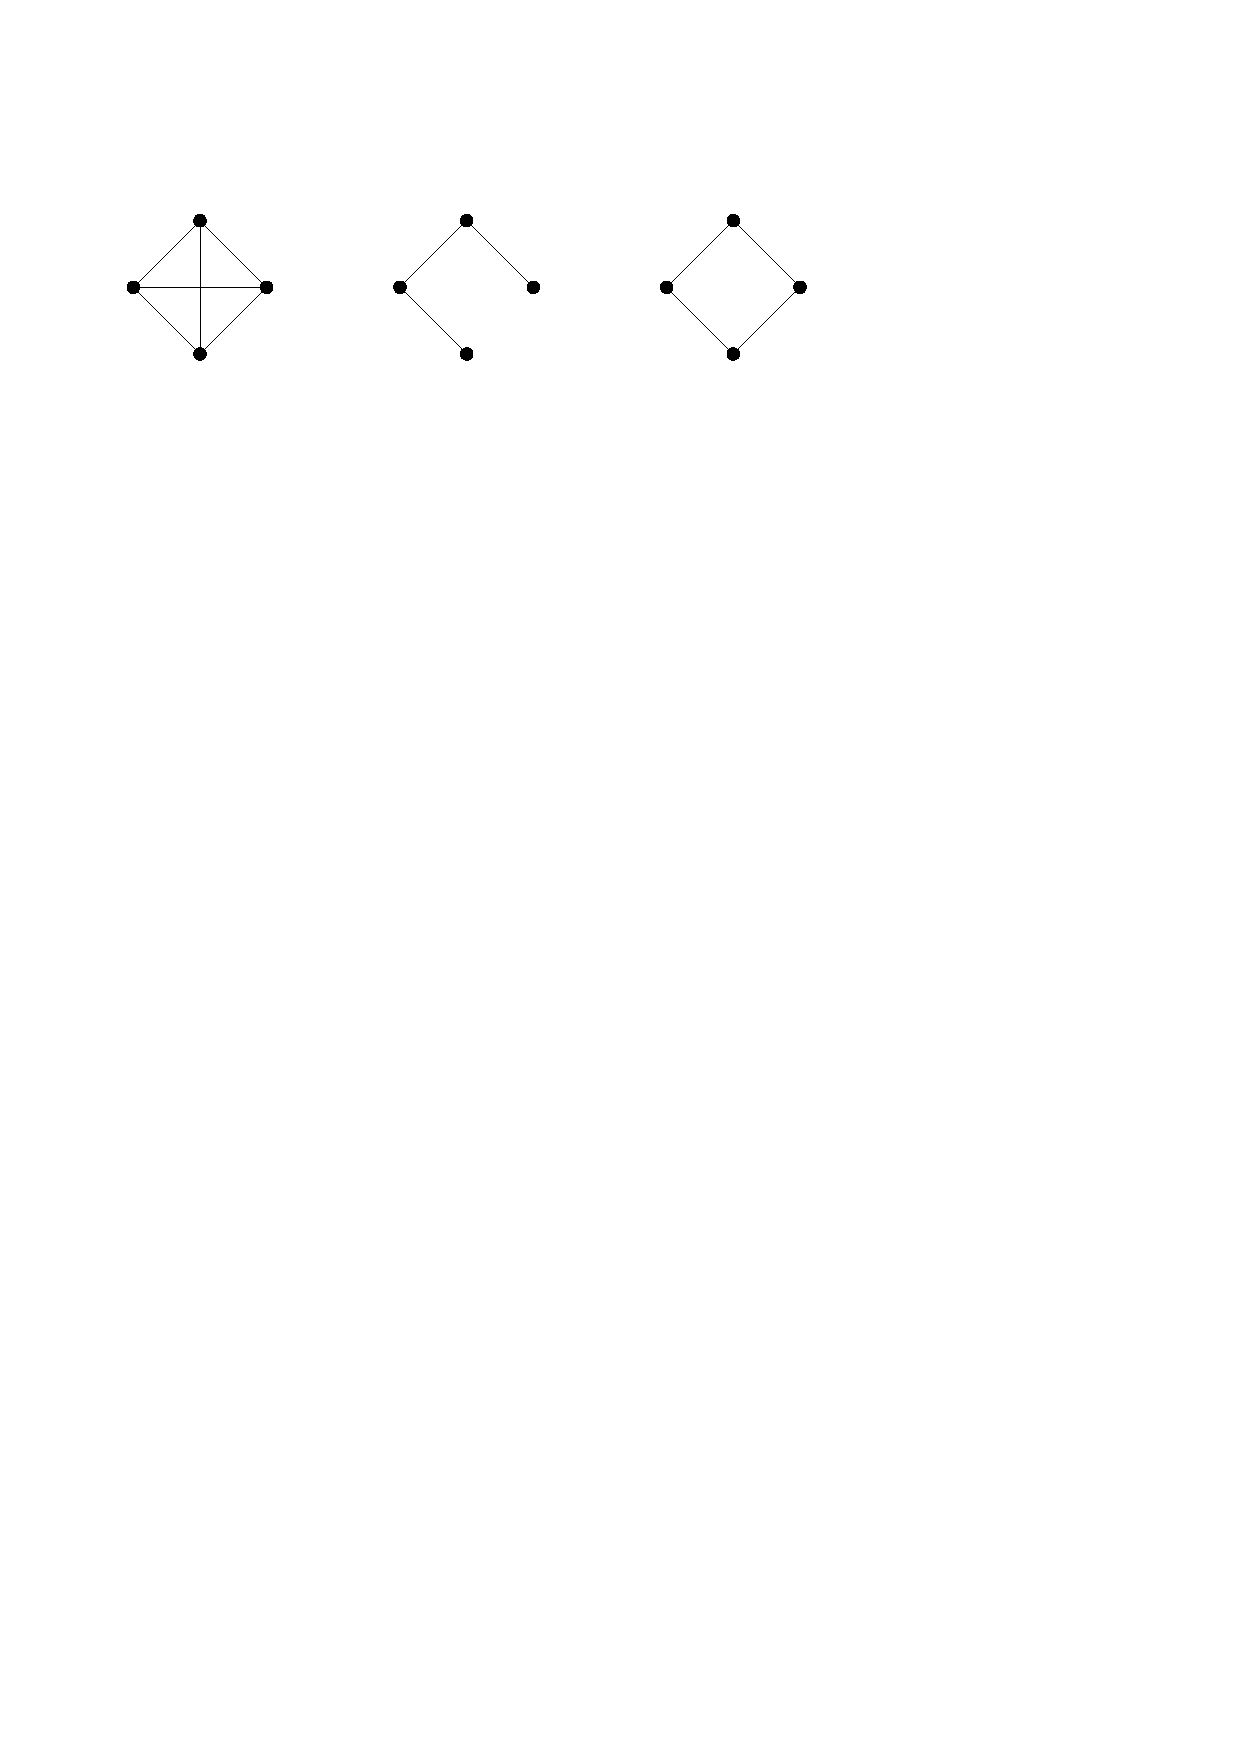
\includegraphics[width=0.6\linewidth]{figures/classic-graphs.pdf}
    \caption{From left to right: complete graph, path graph, cycle graph with 4 vertices.}
    \label{fig:classic-graphs}
\end{figure}

\section{Subgraphs}

\subsection{Definitions}

\begin{definition}[Subgraph]
    Given a graph $G = (V,E)$, a \textit{\textbf{subgraph}} $H$ of $G$ is a pair $H = (W,E')$ such that $W \subseteq V$ and $E' \subseteq \{s \in E \mid s \subseteq W\}$.
\end{definition}

Sometimes, we abuse notation and write $H \subseteq G$.

\begin{definition}[Induced Subgraph]
    Given a graph $G = (V,E)$, an \textit{\textbf{induced subgraph}} $H \subseteq G$ is one of the form $(W,E')$ where
    $$
    E' = \{ \{x,y\} \in E \mid \{x,y\} \in W\}
    $$
    for $W \subseteq V$.
\end{definition}

Note that induced subgraphs are uniquely defined by the vertex set whereas a subgraph is not. A subgraph need not contain all edges between the vertices in the subgraph.

\subsection{Isomorphism}

\begin{definition}[Isomorphic Graphs]
    Let $G = (V_1,E_1)$ and $H = (V_2,E_2)$ be graphs. We say that $G$ and $H$ are isomorphic if there is a bijection $f:\; V_1 \to V_2$ such that $\{x,y\} \in E_1 \iff \{f(x),f(y)\} \in E_2$.
\end{definition}

\begin{theorem}
    Let $G$ be a graph with $n$ vertices. $G$ is isomorphic to a subgraph of $K_n$.
\end{theorem}

\begin{proof}
    Consider $G = (V,E)$. Label the vertices such that $V = \{v_0,\ldots,v_{n-1}\}$. Let $f:\; V \to [n]$ be a function such that $f(v_i) = i$. Consider the set $E' = \{\{i,j\} \subseteq [n] \mid \{v_i,v_j\} \in E\}$. Clearly, $H = ([n], E')$ is a subgraph of $K_n$ by definition. Further, we claim that $f$ is an isomorphism between $G$ and $H$.
    
    To show that $f$ is an isomorphism, it suffices to show that $\{v_i,v_j\} \in E \iff \{f(i),f(j)\} \in E'$. For the forward direction, suppose $\{v_i,v_j\} \in E$, then $\{i,j\} \in E'$ by construction. This immediately implies that $\{f(v_i),f(v_j)\} \in E'$ by construction of $f$. For the reverse direction, suppose $\{i,j\} \in E'$, which is equivalent to $\{f(v_i),f(v_j)\} \in E'$. By definition of $f$, this is only true when $\{v_i,v_j\} \in E$. Therefore, $f$ is an isomorphism between $G$ and $H$.
    
    It follows that $G$ is isomorphic to $H$, which is a subgraph of $K_n$.
\end{proof}

\section{Degrees and Degree Sequence}

\begin{definition}[Degree]
    Given a graph $G = (V,E)$ and a vertex $v \in V$, we let $\deg_G(v) = |\{u \in V \mid \{u,v\} \in E\}|$, which is the number of vertices ahring an edge with $v$.
\end{definition}

\begin{definition}[Degree Sequence]
    Given a graph $G$, we can create a sequence $(\deg_G(v) \mid v \in V)$ of degrees called a degree sequence.
\end{definition}

\begin{theorem}
    Let $G = (V_1,E_1)$ and $H = (V_2,E_2)$ be graphs, and let $f:\; G \to H$ be an isomorphism. Then, $\deg_G(v) = \deg_H(f(v))$.
\end{theorem}

\begin{proof}
    Let $f:\; G \to H$ be an isomorphism. For each $v \in V_1$, consider the sets
    $$
    \{w \in V_1 \mid \{v,w\} \in E_1\}
    $$
    and
    $$
    \{y \in V_2 \mid \{f(v),y\} \in E_2\}.
    $$
    Since $f$ is an isomorphism, each $v \in V_1$ is mapped to one and only one vertex in $V_2$. Further, $\{v,w\} \in E_1 \iff \{f(v),f(w)\} \in E_2$. Then, the two sets have the same cardinality. By definition, this means $\deg_G(v) = \deg_H(f(v))$ for all $v \in V_1$.
\end{proof}

This theorem provides us with a quick way to check if two graphs are isomorphic. We can check this by simply checking the degree and/or degree sequence instead of considering the actual isomorphism mapping.

\begin{corollary}
    If $G$ and $H$ have different degree sequences (under a given ordering of the sequence), then they are not isomorphic.
\end{corollary}

\begin{lemma}[The Handshaking Lemma]
    Let $G=(V,E)$ be a graph, and let $|E| = e$. Then,
    $$
    \sum_{v \in V} \deg_G(v) = 2e
    $$
\end{lemma}

\begin{proof}
    For each $v \in V$, let $E_V = \{\{v,u\} \mid \{v,u\} \in E\}$. Notice that for distinct $u,v$, $|E_u \cap E_v| \leq 1$ and is equal to one exactly when $u$ and $v$ form an edge. No three distinct sets overlap. It follows that
    $$
    e = |E| = \left| \bigcup_{v \in V} E_v \right| = \sum_{v \in V} |E_v| - \sum_{u,v \in V} |E_v \cap E_u| = \sum_{v \in V} \deg_G(v) - e
    $$
    This implies $\sum_{v \in V} \deg_G(v) = 2e$.
\end{proof}

\section{Connectivity}

\begin{definition}[Path]
    A \textit{\textbf{path}} in a graph $G = (V,E)$ is a sequence of \textbf{distinct} vertices $x_1,\ldots,x_n$ that are each successively connected with an edge. We call the number of edges in the sequence the length of the path.
\end{definition}

\begin{definition}[Walk]
    A \textit{\textbf{walk}} in a graph $G = (V,E)$ is a sequence of vertices that are each successively connected with an edge.
\end{definition}

Note that a walk does not have the distinctness requirement, meaning repeating vertices in a walk is allowed.

\begin{definition}[Connectivity]
    We call a graph $G$ connected if every pair of distinct vertices is connected by a path.
\end{definition}

\begin{definition}[Connected Component]
    Given a graph $G$, we call a maximally connected vertex set a \textit{\textbf{connected component}}. More formally, if we denote the equivalence relation $\sim$ on $V$ given by
    $$
    v \sim w \iff v = w
    $$
    (i.e. $v$ is connected to $w$), the \textit{\textbf{connected components}} are the equivalence classes given by this relation.
\end{definition}

\section{Trees and Spanning Trees}

\subsection{Definition and a Useful Theorem}

\begin{definition}[Tree]
    A \textit{\textbf{tree}} is a graph $G = (V,E)$ with the property that every two vertices are connected by a \textbf{unique} path.
\end{definition}

\begin{lemma} \label{lem:acyclic-graph-degree}
    Every acyclic and connected graph $G$ with $n \geq 2$ vertices has a leaf $v \in V$ such that $\deg(v) = 1$.
\end{lemma}

\begin{proof}
    Let $G$ be an acyclic and connected graph. Note that since $G$ is connected, $\deg_G(v) \geq 1$ for all $v \in V$. We prove the contrapositive. Suppose for all $v \in V$, $\deg_G(v) > 1$. Fix a vertex $v$. Starting from $v$, follow a sequence of distinct edges until a vertex repeats. It is possible to visit all vertices without repeating edges because each vertex has two incident edges. Further, because every vertex has degree of at least 2, once we have visited every vertex, there should still be at least one edge unvisited. When we follow that edge, we will arrive at a vertex that has previously been visited. This creates a cycle. So, $G$ is not acyclic.
\end{proof}

\begin{theorem} \label{thm:equiv-tree-def}
    Let $G$ be a \textbf{connected graph} with $n$ edges. The following are equivalent:
    \begin{enumerate}
        \item $G$ is a tree
        \item $G$ does not contain a cycle
        \item $G$ has $n-1$ edges
    \end{enumerate}
\end{theorem}

\begin{proof}
    Let $G$ be a connected graph.

    (1 $\implies$ 2): Assume that $G$ is a tree. We show that $G$ does not contain a cycle by contradiction, so suppose not and $G$ contains a cycle. Let the cycle be $c = x_1x_2\ldots x_n$. Notice that $x_1x_2\ldots x_n$ is a path from $x_1$ to $x_n$. Since $c$ is a cycle, $\{x_1,x_n\} \in E$. So, $x_1x_n$ is also a path from $x_1$ to $x_n$. However, this is a contradiction to the path uniqueness requirement in the definition of a tree. So $G$ does not contain a cycle.

    (2 $\implies$ 3): We prove this implication by induction. Assume $G$ is acyclic and connected.

    \textbf{Base Case}: $n = 1$. There is $0 = n-1$ edge. The implication holds.

    \textbf{Inductive Step}: Let $n \in \N$ and $n \geq 2$. As induction hypothesis, suppose all acyclic and connected graphs with $m \leq n$ vertices have $m-1$ edges. Let $G$ be a graph with $n+1$ vertices. Suppose that $G$ is also connected and acyclic. By Lemma \ref{lem:acyclic-graph-degree}, $G$ has at least one vertex $v$ such that $\deg_G(v) = 1$. Construct $G'$ by removing $v$ and the one edge incident to $v$. $G'$ has $n$ vertices, so by induction hypothesis, has $n-1$ edges. If we add back the removed edge, we can see that $G$ has $n$ edges.

    By induction, this implication holds.

    (3 $\implies$ 1): Let $G$ be a connected graph with $n-1$ edges. To show that $G$ is a tree, we need to show that every two vertices are connected by a unique path. It suffices to show that deleting any edge from $G$ leaves the graph disconnected. Suppose for contradiction that deleting an edge $\{u,v\}$ does not disconnect the graph. This implies that there is another path from $u$ to $v$ containing at least 2 edges. This also implies that $G$ is connected with $n-2$ edges. But this is impossible because the minimum number of edges in a connected graph with $n$ vertices is $n-1$. Therefore, every pair of vertices is connected via a unique path since deleting any edge breaks this path and thus disconnects the graph. By definition, this means $G$ is a tree.
\end{proof}

\begin{definition}
    Let $T = (V,E)$ be a tree. We call a vertex $v$ a leaf if $\deg_T(v) = 1$.
\end{definition}

\begin{lemma}
    If $G = (V,E)$ is a tree with $n \geq 2$ vertices, then $G$ has at least two leaves.
\end{lemma}

\begin{proof}
    We prove this lemma by strong induction on $n$ for $n \geq 2$.

    \textbf{Base Case}: $n = 2$. Since $T$ is a tree, $T$ is connected and has exactly one edge. Clearly, both vertices in $T$ have degree 1.

    \textbf{Inductive Step}: Suppose, as inductive hypothesis, that for some $n \geq 2$, every tree with $2 \leq k \leq n$ vertices has at least two leaves. Let $T$ be a tree with $n+1$ vertices. Pick an edge $\{u,v\} \in E$ and form a new graph $T'$ by deleting $\{u,v\}$. More formally, $T' = (V, E - \{\{u,v\}\})$. Since $T$ is a tree, there is no other path between $u$ and $v$ (otherwise we would have a cycle). It follows that in $T'$, $u$ and $v$ are disconnected. Deleting an edge will not create a cycle either, so $T'$ is a forest with two connected components $T_u$ and $T_v$. Consider the following cases:

    Case 1: Both $T_u$ and $T_v$ contain at least 2 vertices. Then, we can apply our induction hypothesis. Take one leaf from each component. If both are endpoints of the deleted edge $\{u,v\}$, they are no longer leaves in $T$, but we still have at least two leaves, one from $T_u$ and one from $T_v$. In general, $T_u$ must have a leaf $x$ that is not $u$ and $T_v$ must have a leaf $y$ that is not $v$. Adding $\{u,v\}$ back does not affect $x$ and $y$ so they will remain leaves, which implies that there exist at least two leaves.
    
    Case 2: If each component of $T'$ has only one vertex, then $T$ is isomorphic to $K_2$, which has two leaves.
    
    Case 3: If exactly one of the components has only one vertex, then it must become a leaf when we reconnect $\{u,v\}$ to form $T$.

    In all cases, we have that $T$ has at least two leaves. By induction, every tree with at least 2 vertices has at least two leaves.
\end{proof}

\begin{figure}[htbp]
    \centering
    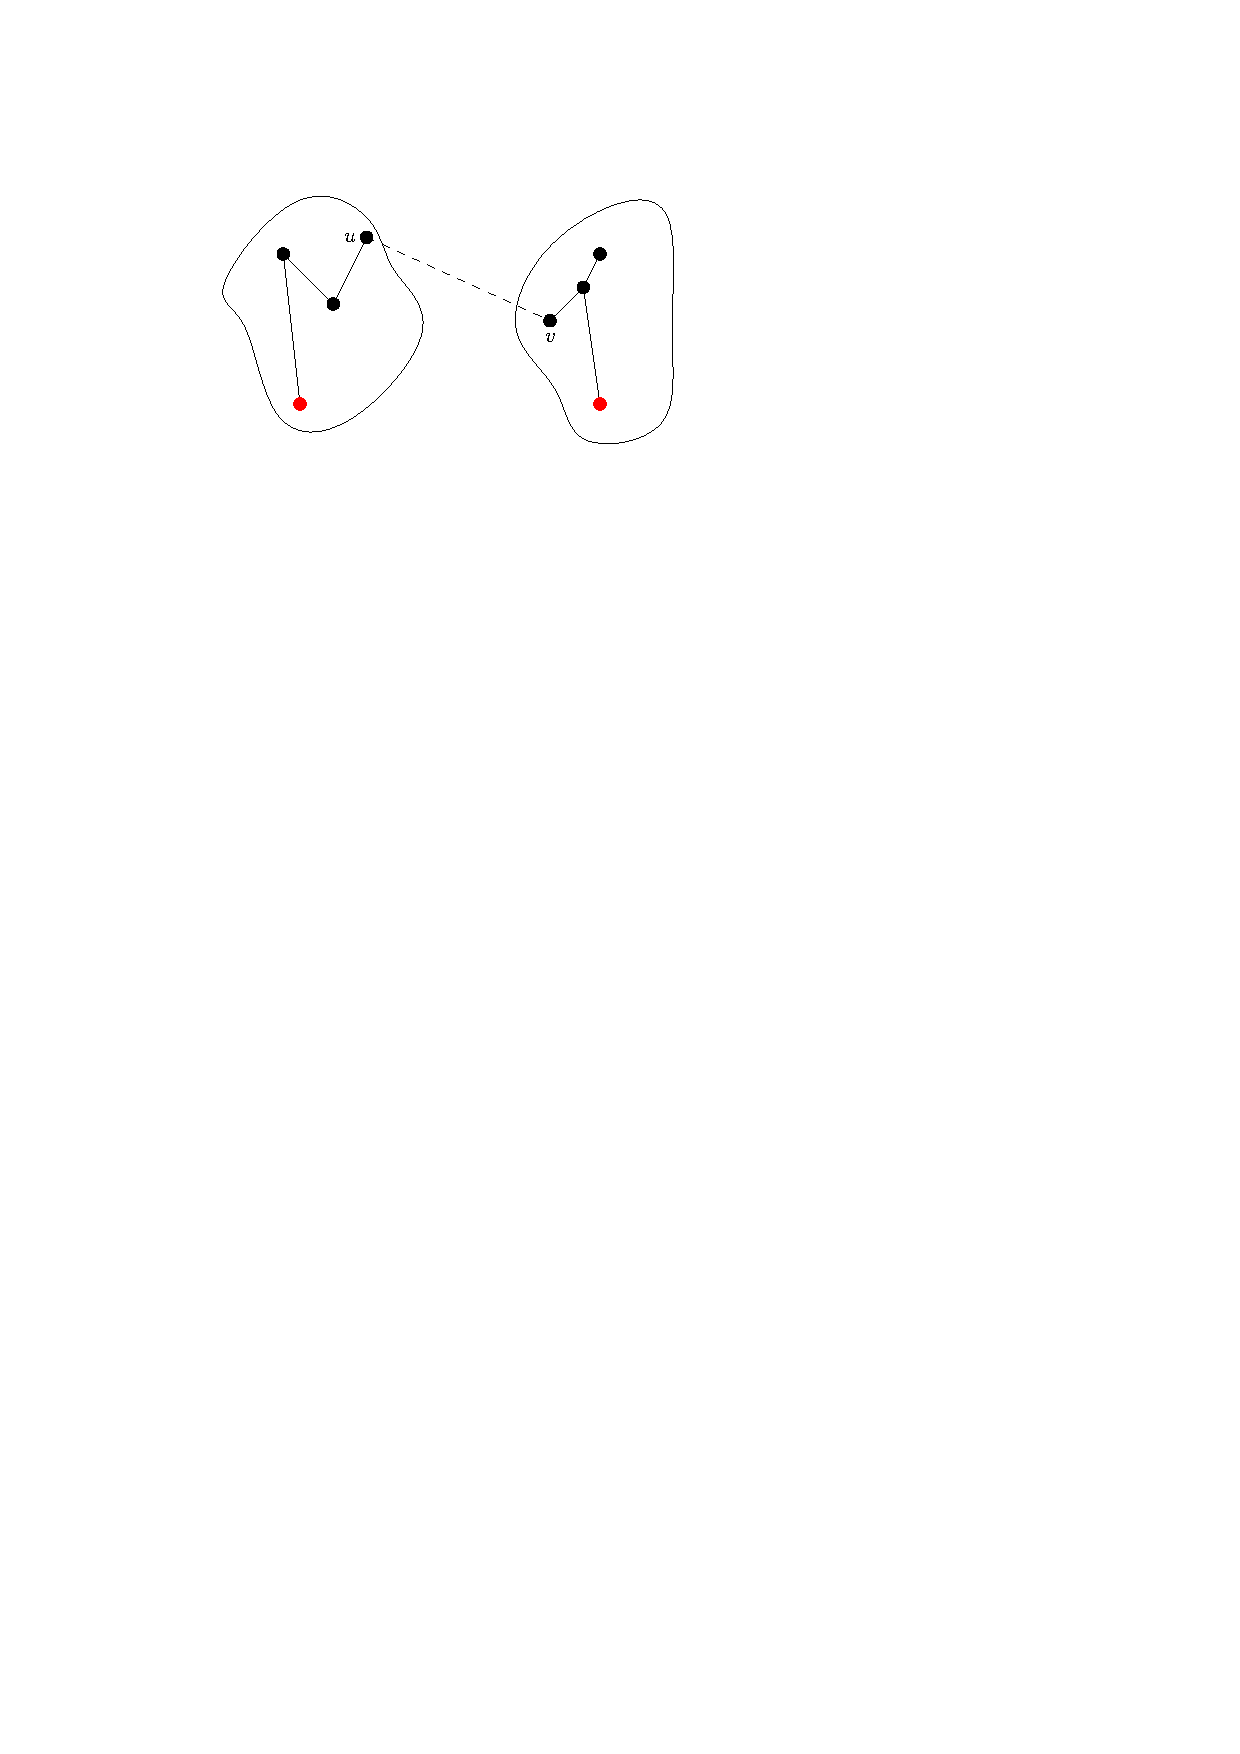
\includegraphics[width=0.4\linewidth]{figures/pendant-vertex-cycle.pdf}
    \caption{In each of the two components, there exists at least one leaf that is not $u$ or $v$ (colored red). When we reconnect $\{u,v\}$, those vertices will remain leaves.}
    \label{fig:pendant-vertex}
\end{figure}

\subsection{Spanning Trees}

\begin{definition}[Spanning Subgraph]
    Given a graph $G = (V,E)$, we call a subgraph $H \subseteq G$ \textit{\textbf{spanning}} if $H = (V,E')$.
\end{definition}

\begin{definition}[Spanning Tree]
    Given a graph $G$, a \textit{\textbf{spanning tree}} is a spanning subgraph $T \subseteq G$ that is a tree.
\end{definition}

\begin{theorem}
    Every connected graph has a spanning tree.
\end{theorem}

\begin{proof}
    By induction on the number of edges.

    \textbf{Base Case}: If $G$ is connected and has no edges, $G$ contains one single vertex. $G$ is trivially a tree and a spanning tree.

    \textbf{Inductive Step}: Suppose $G$ has $m \geq 1$ edges. If $G$ is a tree, then we are done because it is trivially a spanning tree. Otherwise, $G$ has cycles. For each cycle, remove an edge from the cycle to disconnect the cycle. By definition of a cycle, the graph is still connected after the removal of edges from the cycles. The resulting graph is still connected but has no cycle, which by Theorem \ref{thm:equiv-tree-def}, means the resulting graph is a tree. By definition of a spanning tree, this means the resulting graph is a spanning tree.

    By induction, a connected graph with $n$ edges has a spanning tree for all $n \in \N$. This implies that all connected graphs have a spanning tree.
\end{proof}

\chapter{Eulerian and Hamiltonian Graphs}
\section{Eulerian Graphs and Circuit}

\begin{definition}[Eulerian Circuit]
    Given a graph $G = (V,E)$, an \textit{\textbf{Eulerian circuit}} is a sequence of vertices $x_0,\ldots,x_t$ such that
    \begin{itemize}
        \item $x_0 = x_t$ 
        \item $\forall i \in [t].\, \{x_i, x_{i+1}\} \in E$ 
        \item $\forall e \in E.\, \exists \text{ unique $i \in [t]$.}\, e = \{x_i, x_{i+1}\}$ (i.e. every edge appears exactly once in an Eulerian circuit)
    \end{itemize}
\end{definition}

We say a graph is \textit{\textbf{Eulerian}} if and only if it has an \textbf{Eulerian circuit}. An Eulerian circuit is also referred to as an \textbf{Euler tour} in some texts. The notion of an Eulerian circuit and graph appears in the famous problem of the \textbf{bridges of K\"onigsberg}.

In 1736, Euler gave his famous characterization of an Eulerian graph, stated as follows

\begin{theorem}[Euler, 1736]
    A connected graph $G = (V,E)$ is Eulerian if and only if all its vertices have even degree.
\end{theorem}

\begin{proof}
    The forward direction of the proof is quite straightforward whereas the reverse direction requires a slightly more involved proof by induction.

    ($\implies$): Let $G$ be a connected graph. Assume that $G$ is Eulerian so it must have an Eulerian circuit. Note that in an Eulerian circuit, every time we enter a vertex, we must also leave the vertex. This is the case for all vertices because otherwise we would have an infinite graph. Hence, all vertices in $G$ must have even degree.

    $(\impliedby)$: Let $G$ be a graph. We proceed by strong induction on the number of edges.

    \textbf{Base Case}: $G$ is a graph with $m = 0$ edge. The result trivially holds.

    \textbf{Inductive Step}: Let $m \in \N$ be arbitrary. Assume that for all $k \in \N$ such that $0 \leq k < m$, the implication holds. Let $G = (V,E)$ be a connected graph with $m$ edges. Further, assume that $\deg_G(v)$ is even for all $v \in V$. Since the graph is connected and every vertex has even degree, it follows immediately that $\deg_G(v) \geq 2$ for all $v \in V$. This also implies that $G$ contains a cycle. Let $c = v_1\ldots v_k$ be such cycle of maximal length and $E'$ be the edges contained in this cycle.

    If $c$ contains all edges exactly once, we are done. Hence, suppose $E' \neq E$ and consider the graph $G' = (V, E \setminus E')$. It has connected components $S_1, \ldots, S_l$. Since $E' \neq E$, each of the connected components $S_i$ contains strictly fewer edges than $|E| = m$. For every $v \in G$, an even number of edges of $G$ at $v$ are in the cycle $c$, so we we remove these edges, each vertex in the remaining graph should still have even degree. Apply the induction hypothesis to the components, which asserts that each of the components $S_1, \ldots, S_l$ possess an Eulerian circuit. Further, since $c$ is a cycle, $C = (\{v_1,\ldots,v_k\}, E')$ itself is also Eulerian. Now, we recursively construct an Eulerian circuit, say $x$, in the original graph $G$. Start from $v_1$, find the component $S_i$ containing $v_1$, and concatenate the Eulerian tour in $S_i$ to $x$. Next, move from $v_1$ to $v_2$ along $\{v_1,v_2\} \in E'$. If $\{v_1,v_2\} \not\in E$, then they must have been in the same connected component, in which case we skip $v_2$ and move to $v_3$. Repeat this until we have walked through every edge in each one of the $l$ connected components and the edges in $E'$ connecting each component. It is clear that $x$ is Eulerian since it visits every edge exactly once.

    By induction, the implication holds.
\end{proof}

\begin{figure}[htbp]
    \centering
    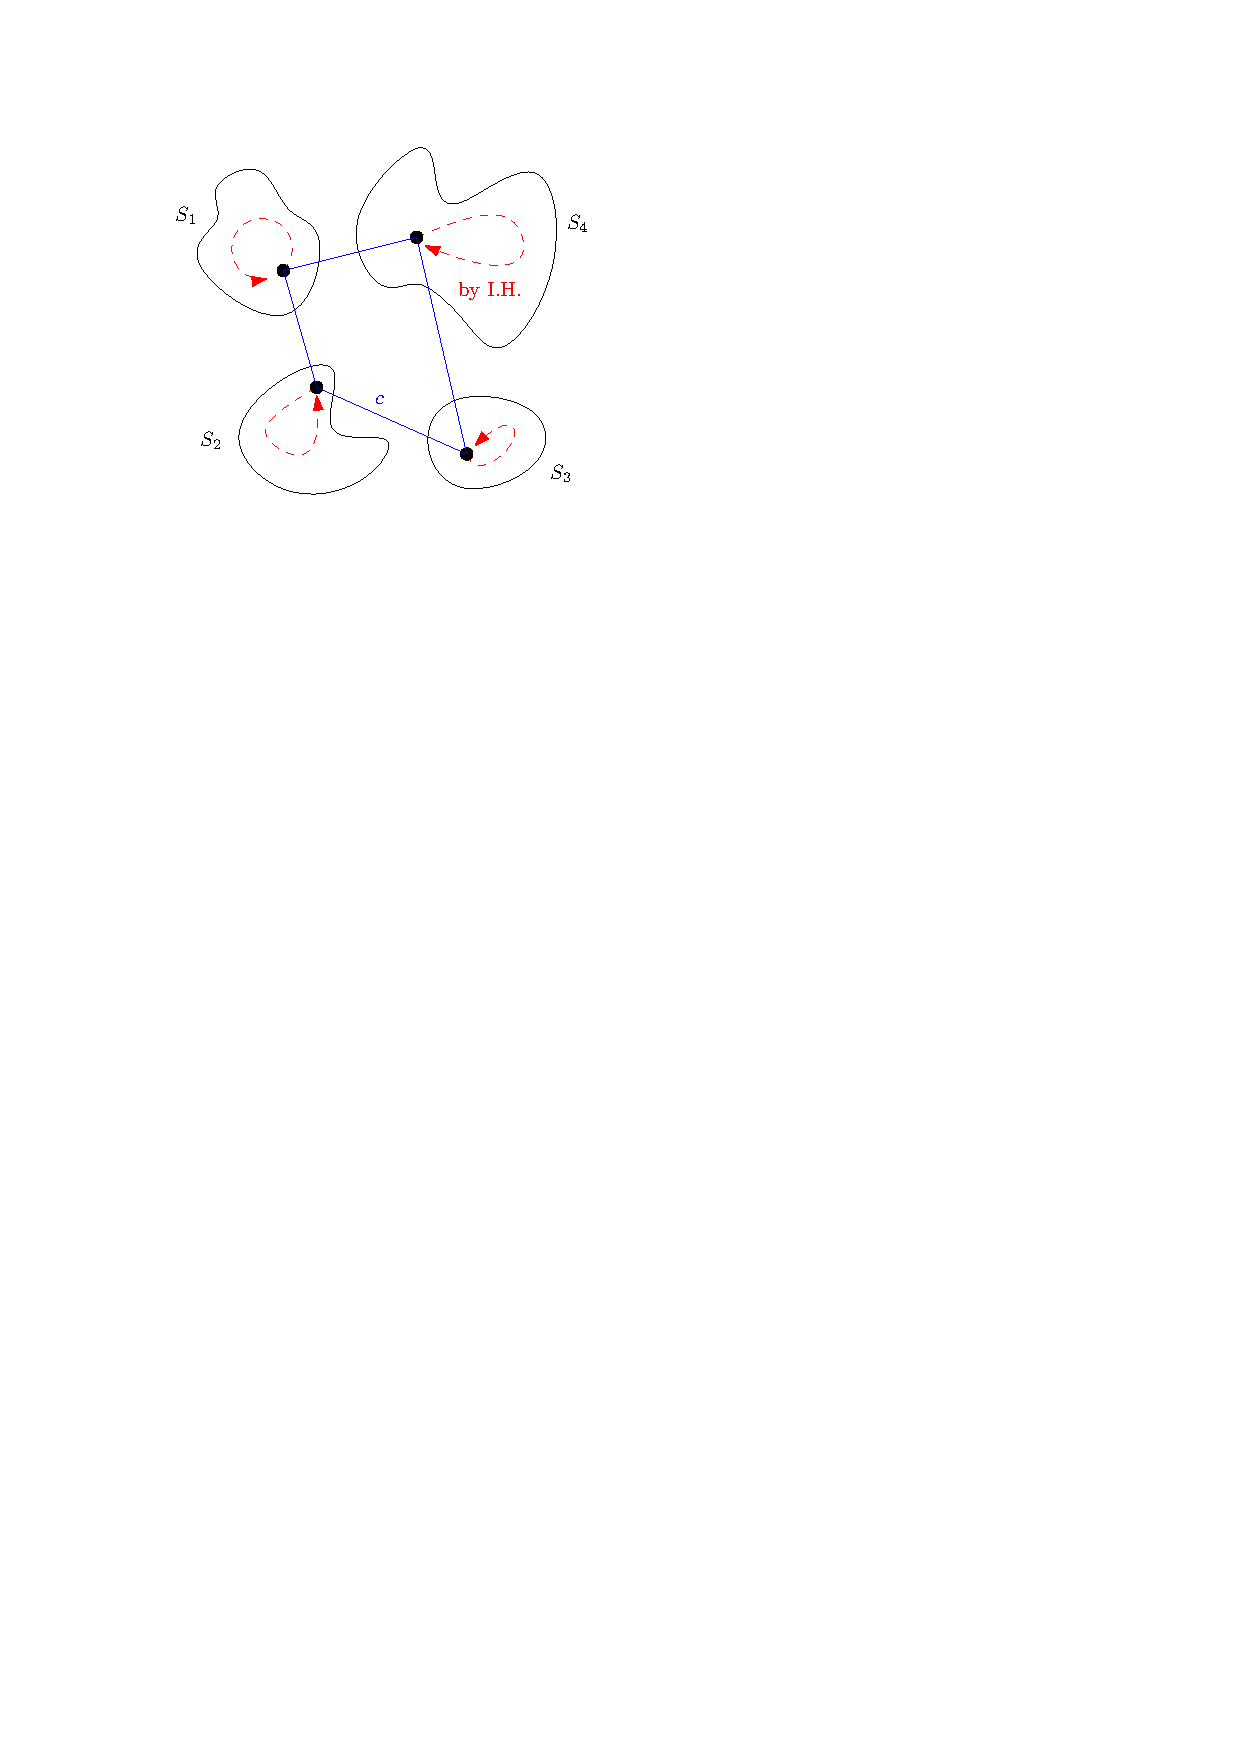
\includegraphics[width=0.3\linewidth]{figures/eulerian-circuit-construct.pdf}
    \caption{Construct an Eulerian circuit in the original graph $G$ by first finding a cycle $c$, remove the cycle, find an Eulerian circuit within each component $S_1,\ldots,S_l$, and concatenate these circuits via the cycle $c$.}
    \label{fig:euler-circuit-construct}
\end{figure}

\section{Hamiltonian Graphs}

\begin{definition}[Circuits]
    A \textit{\textbf{circuit}} in a graph $G = (V,E)$ is a sequence of distinct vertices $v_1,\ldots,v_k$ such that for all $i \in \{1,\ldots, k-1\}$, $\{v_i,v_{i+1}\} \in E$ and $\{v_k,v_1\} \in E$. Note, a circuit induces a copy of a subgraph isomorphic to $C_k$ for $k \geq 3$. Specially, we define a \textbf{single vertex} a circuit as well.
\end{definition}

\begin{definition}[Hamiltonian Graph]
    We call a graph with $n$ vertices \textit{\textbf{Hamiltonian}} if it admits a circuit of length $n$, which is to say that the graph has a spanning subgraph that is isomorphic to $C_n$.
\end{definition}

A sufficient condition for Hamiltonian graphs.

\begin{theorem}[Dirac, 1952]
    Let $G = (V,E)$ be a graph with $n$ vertices where $n \geq 3$. Suppose that for every $v \in V$, $\deg_G(v) \geq \ceil{\frac{n}{2}}$. Then, $G$ is Hamiltonian.
\end{theorem}

\begin{proof}
    Let $G = (V,E)$ be a graph with $n \geq 3$ vertices. Assume that $\deg_G(v) \geq \ceil{\frac{n}{2}}$ for all $v \in V$. Let $\delta(G)$ denote the minimum degree. That is, $\delta(G) = \min \{\deg_G(v) \mid v \in V\}$. Then, the assumption is equivalent to that $\delta(G) \geq \ceil{\frac{n}{2}}$.
    
    We claim that $G$ is connected. We prove the claim by contradiction. So suppose not, consider the component $G' = (V_{G'}, E_{G'})$ of $G$ with the fewest number of vertices. Since $\delta(G) \geq \ceil{\frac{n}{2}}$, each vertex is connected to at least $\ceil{\frac{n}{2}}$ other vertices. Since $C$ is a component that is not connected to vertices in other components, $|V_{G'}| \leq \ceil{\frac{n}{2}}$. But then, $\delta(G') < |V_C| \leq \ceil{\frac{n}{2}}$, which contradicts the assumption that $\deg_G(v) \geq \ceil{\frac{n}{2}}$ for all $v \in V$, including those in $G'$.

    Since $G$ is connected, we can find the longest path in $G$. Let $P = v_0 \ldots v_k$ be a longest path in $G$ of length $k$ (with $k$ edges and $k+1$ vertices). We claim that there exists some $0 \leq i \leq k-1$ such that $\{v_0,v_{i+1}\} \in E$, $\{v_i, v_k\} \in E$, and $\{v_i, v_{i+1}\} \in E$ as shown in Figure \ref{fig:dirac-thm-path}.

    \begin{figure}[htbp]
        \centering
        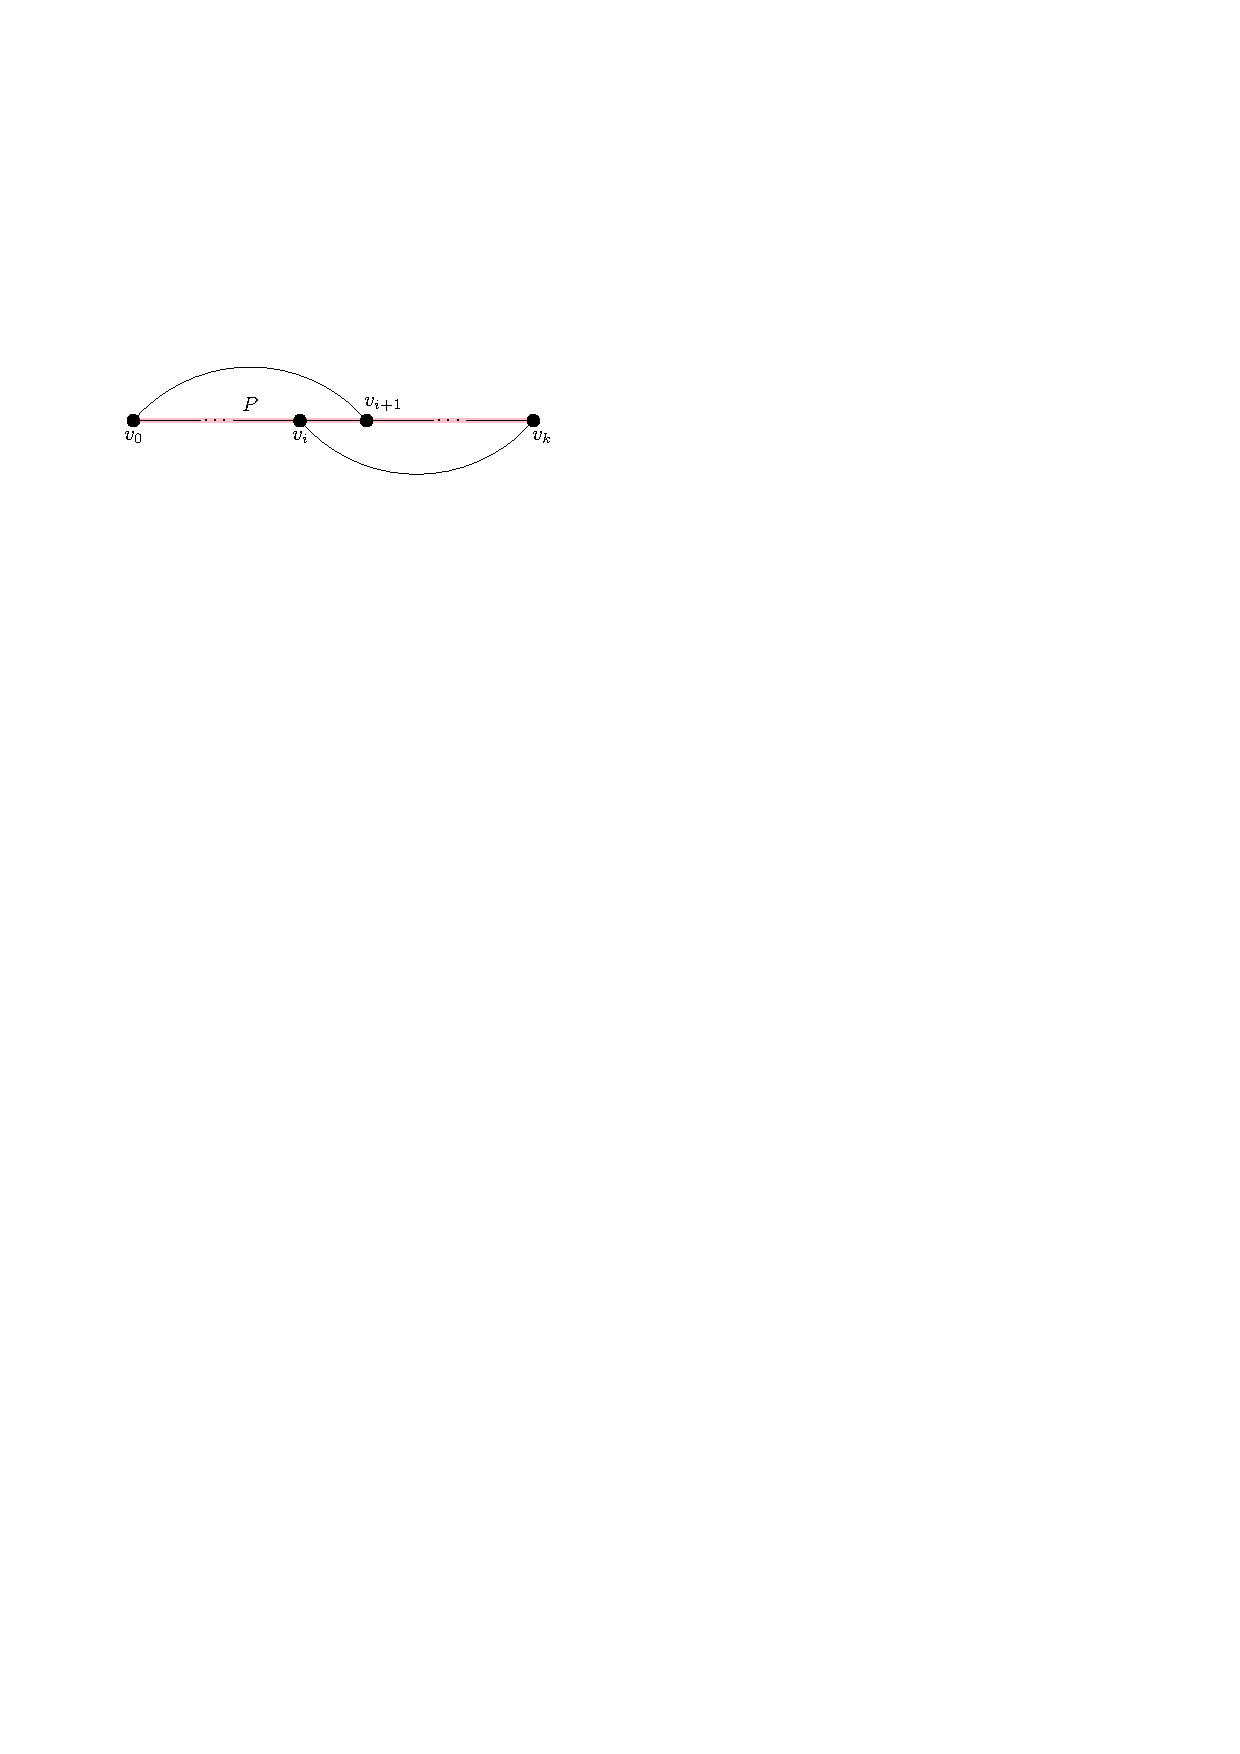
\includegraphics[width=0.4\linewidth]{figures/dirac-thm-path.pdf}
        \caption{The longest path $P = v_0\ldots v_k$ with $k+1$ vertices is colored in red. There exists some $0 \leq i \leq k$ such that $\{v_0,v_{i+1}\} \in E$ and $\{v_i,v_k\} \in E$.}
        \label{fig:dirac-thm-path}
    \end{figure}

    Such adjacent vertices $v_i$ and $v_{i+1}$ such that $v_i$ is adjacent to $v_k$ and $v_{i+1}$ is adjacent to $v_0$ must exists. By way of contradiction, suppose $v_i$ and $v_{i+1}$ do not exist. Then, for every vertex adjacent to $v_0$, there must exists some vertex adjacent to it that is NOT adjacent to $v_k$. Similarly, for every vertex adjacent to $v_k$, there must exists some adjacent vertex that is NOT adjacent to $v_0$. Note that these two sets of vertices are disjoint and do not include $v_k$. This implies that
    $$
    \deg_G(v_0) + \deg_G(v_k) + 1 \leq k + 1
    $$
    since we are not overcounting and the number of vertices being counted is at most the length of path $P$. The additional 1 on the LHS of the inequality came from couting $v_k$ as it is not included in either $\deg_G(v_0)$ or $\deg_G(v_k)$. Now, since $\deg_G(v) \leq \ceil{\frac{n}{2}}$ for all $v \in V$,
    $$
    n + 1 \leq \left\lceil \frac{n}{2} \right\rceil + \left\lceil \frac{n}{2} \right\rceil + 1 \leq \deg_G(v_0) + \deg_G(v_k) + 1 \leq k + 1
    $$
    so $n + 1 \leq k+1$. This implies that $n < k+1$ since both $n$ and $k$ are integers. But this leads to a contradiction because the number of vertices on the path $P$ cannot be more than the total number of vertices in the entire graph.

    The existence of such $v_i$ and $v_{i+1}$ allows us to construct a cycle $C = v_0 \to v_{i+1} \leadsto_{P} v_k \to v_i \leadsto_{P} v_0$. We claim this cycle is Hamiltonian.

    \begin{figure}[htbp]
        \centering
        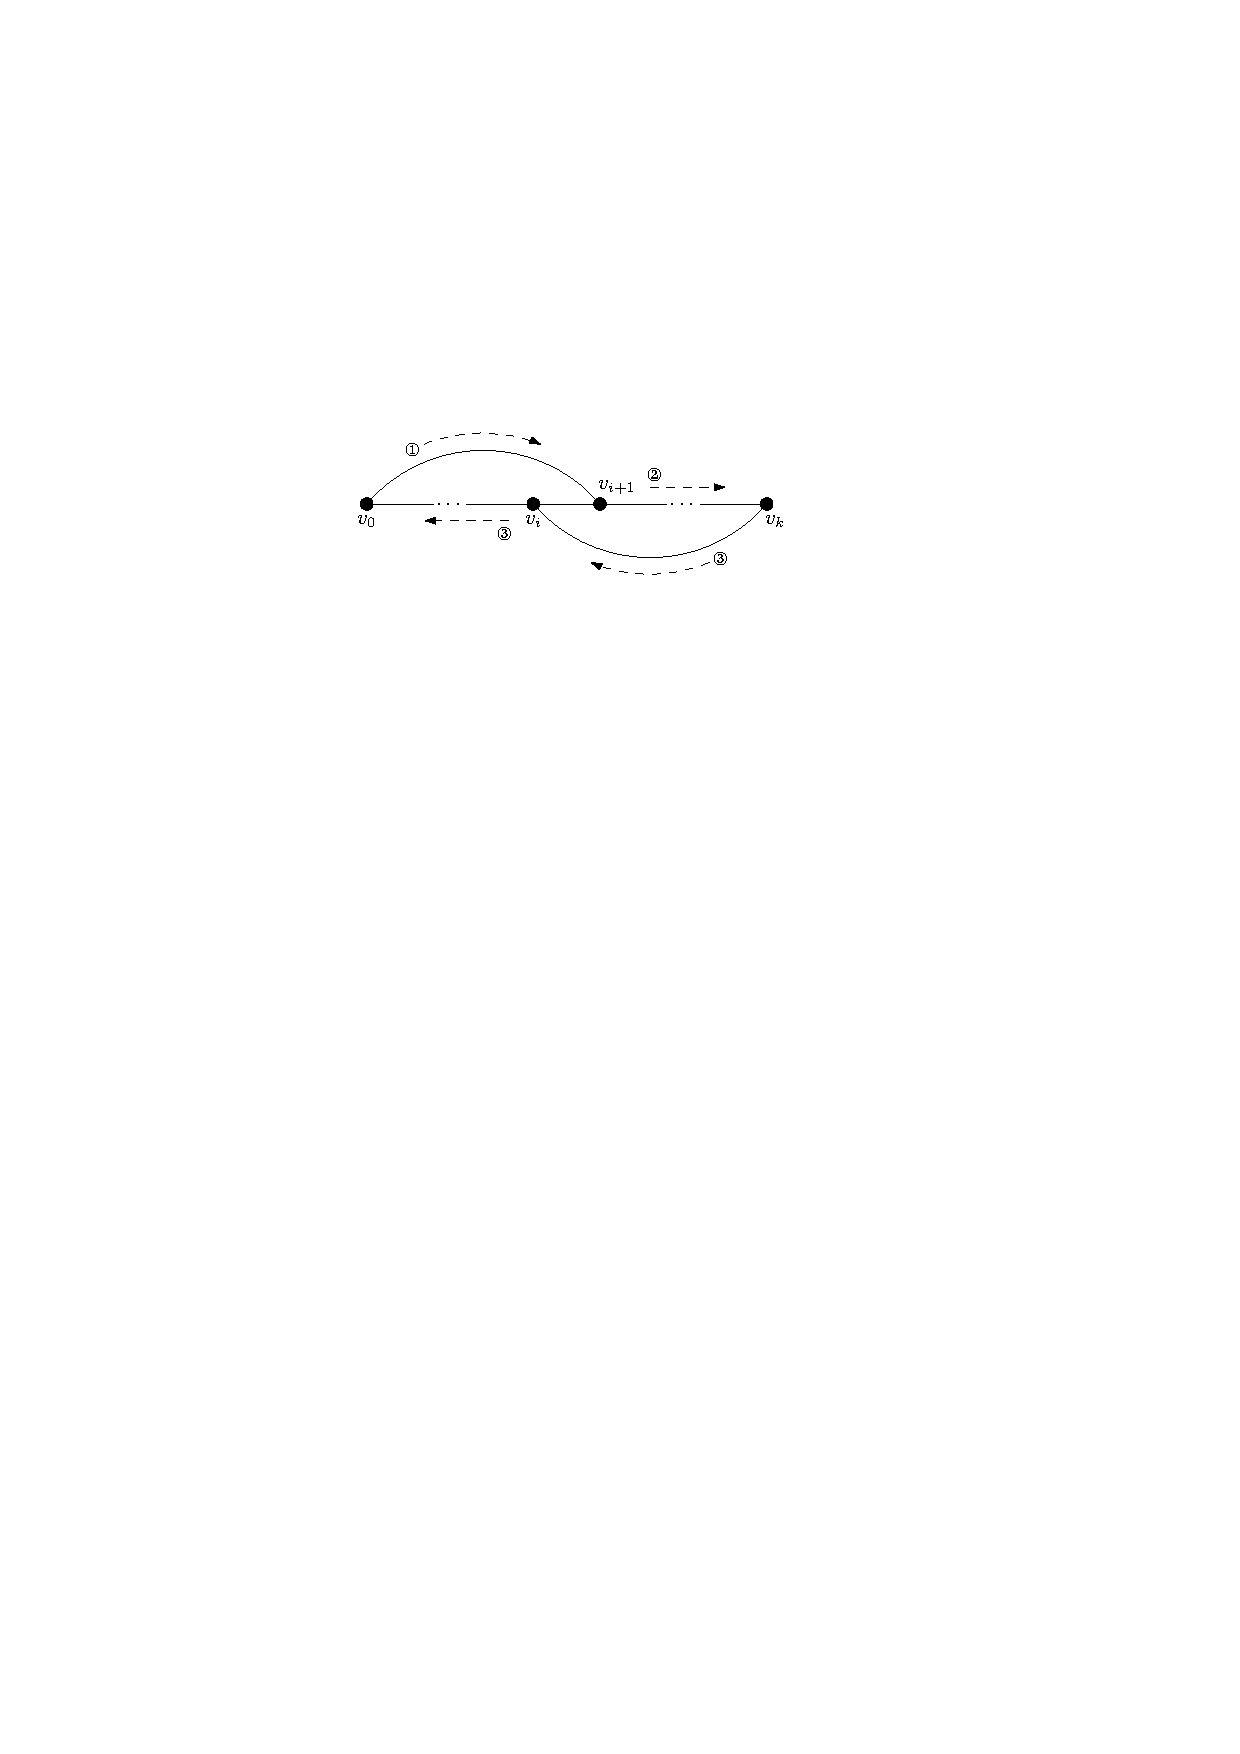
\includegraphics[width=0.4\linewidth]{figures/dirac-thm-hamcycle.pdf}
        \caption{The Hamiltonian path is $C = v_0 \to v_{i+1} \leadsto_{P} v_k \to v_i \leadsto_{P} v_0$.}
        \label{fig:dirac-thm-hamcycle}
    \end{figure}

    To see why $C$ is Hamiltonian, again we use a contradiction proof. Suppose $C$ is not Hamiltonian. Then, by definition, there must be some vertex $w \in V$ such that $w$ is not on $C$. But since $G$ is connected, $w$ must be adjacent to some vertices, say $v_w \in V$. Without loss of generality, suppose that this $v_w$ is on the cycle $C$. There must also be a $v_{w+1}$ immediately adjacent to $v_w$. By construction, the cycle $C$ contains $k+1$ edges (that's all edges on $P$ along with $\{v_0,v_{i+1}\}, \{v_i,v_k\}$ and without $\{v_i,v_{i+1}\}$). We then consider the path from $v_w$ to $v_{w+1}$ by following the edges on the cycle. This leads to a path of length $k$, namely $p = v_w \leadsto v_0 \to v_{i+1} \leadsto v_k \to v_i \leadsto v_{w+1}$. Now, we extend the left end of this path to $w$ since $w$ is adjacent to $v_w$ and still get back a valid path. The new path $P' = w \to v_w \leadsto v_0 \to v_{i+1} \leadsto v_k \to v_i \leadsto v_{w+1}$ is one edge longer than $p$. However, this contradicts the maximality assumption for $P$ since now we would have a path, $P'$, that contains more vertices than $P$. Therefore, $C$ is indeed a Hamiltonian path.

    \begin{figure}[htbp]
        \centering
        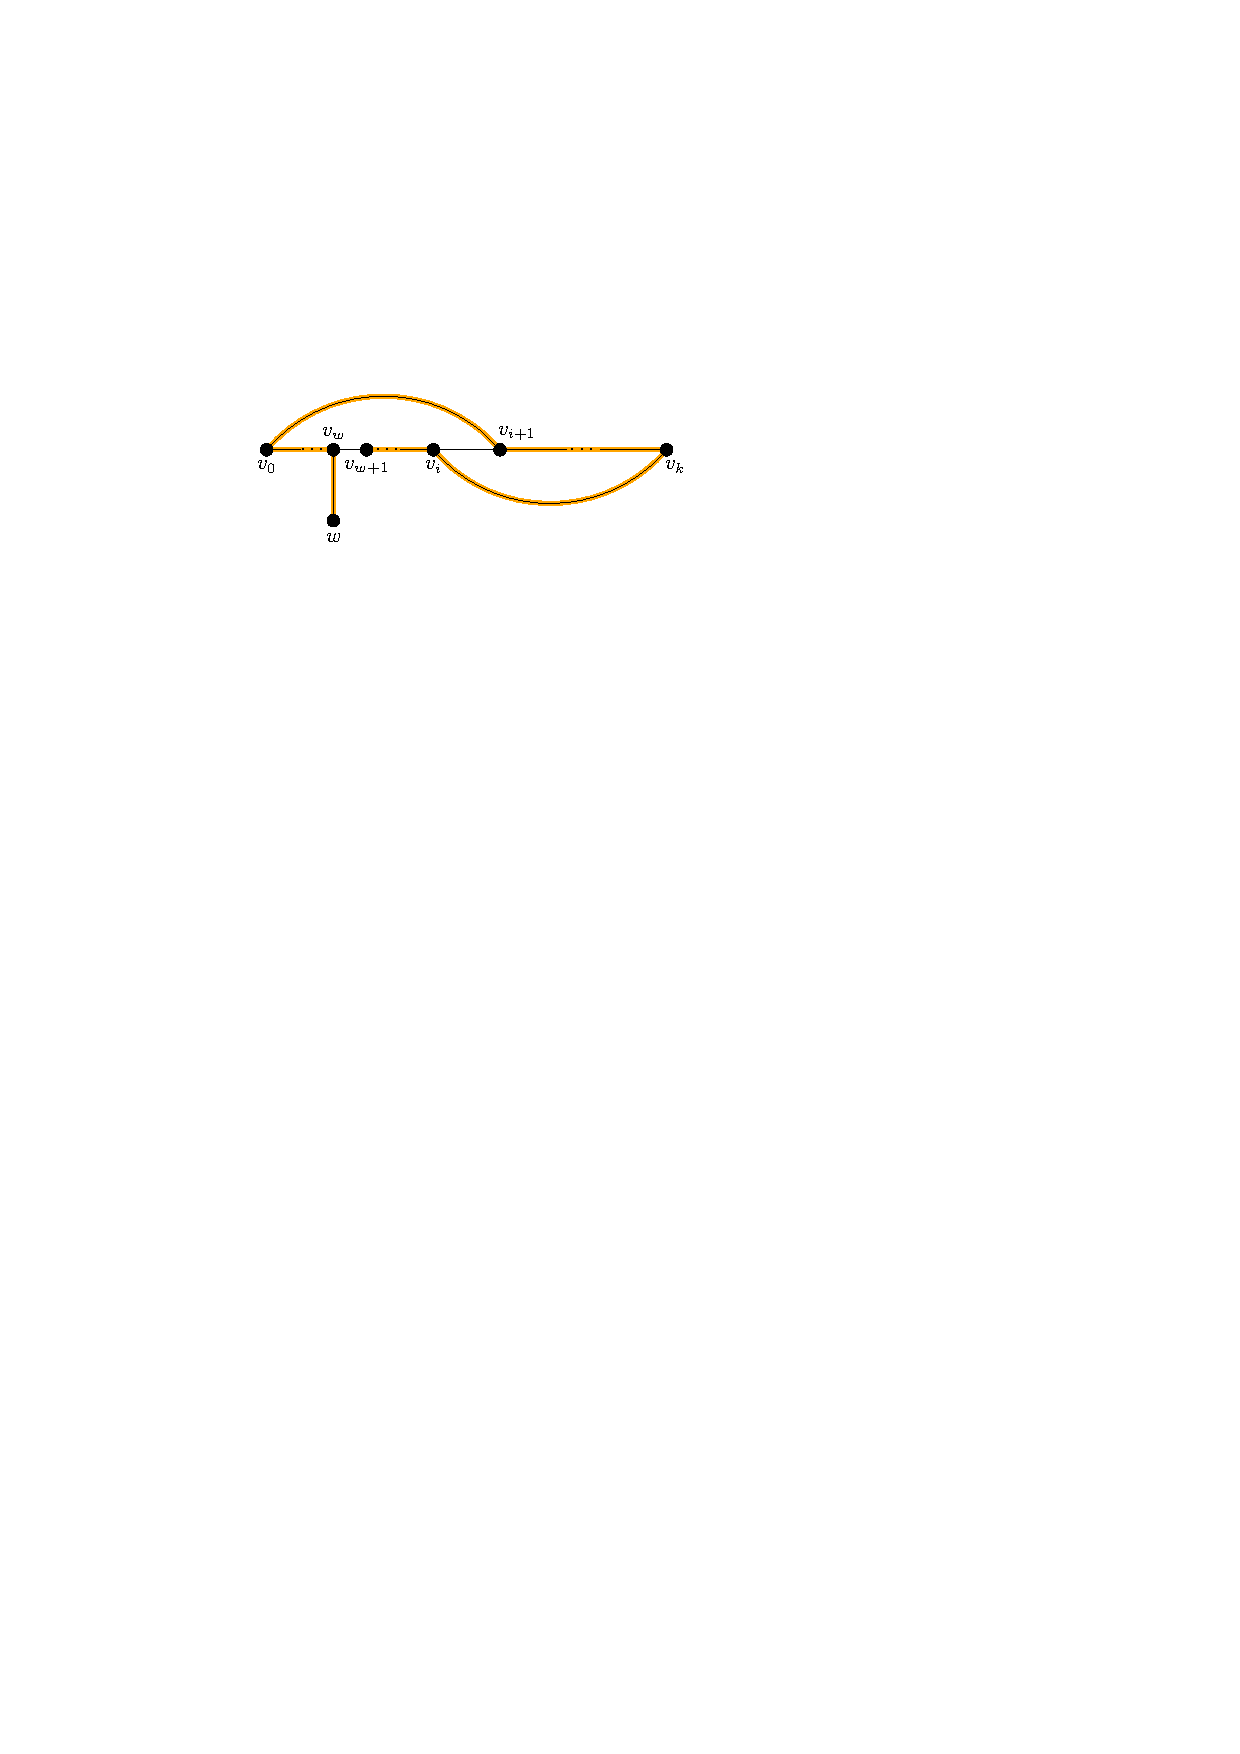
\includegraphics[width=0.4\linewidth]{figures/dirac-thm-longer-path-contradiction.pdf}
        \caption{With the existence of a vertex $w$ outside of the previously constructed cycle, we would have a longer path (colored in orange), contradicting the maximality of $P$.}
        \label{fig:dirac-thm-path-contradiction}
    \end{figure}

    It follows immediately that $G$ is Hamiltonian by definition.
\end{proof}

\chapter{Graph Coloring}
\section{Graph Coloring}

\subsection{Independent Sets and Bipartite Graphs}

\begin{definition}[Independent Set]
    Given a graph $G = (V,E)$, we say $A \subseteq V$ is \textit{\textbf{independent}} if and only if no no vertices in $A$ are adjacent.
\end{definition}

The only independent sets in $K_n$ are singletons. We can prove this using a contradiction and the definition of a complete graph and independent set.

\begin{definition}[Bipartite Graph]
    We say a graph $G = (V,E)$ is \textit{\textbf{bipartite}} if and only if we can partition $V$ into two \textbf{disjoint} \textbf{independent} sets.
\end{definition}

A bipartite graph $(V_1 \cup V_2, E)$ is a complete bipartite graph iff every $v_1 \in V_1$ is connected to every vertex in $V_2$ and vice versa. We denote a complete bipartite graph by $K_{|V_1|,|V_2|}$ ($K$ with a subscript denoting the size of the left and right partition, respectively).

\begin{theorem} \label{thm:odd-length-cycle-bipartite}
    A graph is bipartite if and only it does not contain a circuit of odd length.
\end{theorem}

\begin{proof}
    \hfill

    ($\implies$): Let $G=(V,E)$ be a bipartite graph. In particular, $V = A \cup B$ for some $A,B \subseteq V$ such that $A \cap B = \emptyset$ and for all $\{a,b\} \in E$, $a \in A$ and $b \in B$. Suppose, for contradiction, that $G$ contains an odd-length cycle $C = v_1 v_2 \ldots v_{n} v_1$ of length $n$. Without loss of generality, suppose that $v_i$ and $v_{i+1}$ alternates between $A$ and $B$. So, $v_1 \in A$, $v_2 \in B$, $v_3 \in A$, and so on. If the cycle is not in that particular order, we can reindex the vertices and still have the same cycle.

    Then, for $k \in \{1,2,3,\ldots,n\}$,
    $$
    v_k \in \begin{cases}
        A & \text{$k$ is odd} \\
        B & \text{$k$ is even}
    \end{cases}
    $$
    Since $C$ is a cycle of odd length, $n$ is odd. It follows that $v_n \in A$. But then, since $v_1 \in A$ and $\{v_n, v_1\} \in E$, this is a contradiction to the assumption that $G$ is bipartite.

    ($\impliedby$): Let $G=(V,E)$ be a graph. Without loss of generality, assume that $G$ is connected. Otherwise, we can consider the connected components individually. Assume that $G$ contains no odd cycle. Let $w \in V$ be a vertex in $G$.

    Let $A$ be the set of vertices whose shortest distance from $w$ is even, and let $B$ be the set of vertices whose shortest distance from $w$ is odd. That is,
    $$
    \begin{aligned}
        A = \{ v \in V \mid d(v,w) \equiv 0 \mod 2 \} \\
        B = \{ v \in V \mid d(v,w) \equiv 1 \mod 2 \}
    \end{aligned}
    $$
    Since $G$ is connected, every vertex is either at an even distance or odd distance from $w \in V$. A vertex cannot be both at an even distance and an odd distance from $w$ at the same time. Hence, $A \cup B = V$ and $A \cap B = \emptyset$. This implies that $A$ and $B$ are a valid partition of $V$.
    
    Now, we would like to show that $G$ is bipartite. It suffices to show for all vertices $a_1,a_2 \in V$ and $b_1,b_2 \in B$, $\{a_1,a_2\} \not\in E$ and $\{b_1,b_2\} \not\in E$. To prove this fact, we suppose the contrary and derive a contradiction. So, suppose that there does exist such $x,y \in A$ or $x,y \in B$ such that $\{x,y\} \in E$. Fix such $x,y$. We can assume that $x \neq y \neq w$. Otherwise, we have $w = x$ and $d(x,w) = 0$. Since $x$ and $y$ are in the same partition, $d(y,w)$ is even and $d(y,x) = 0$. However, this is not possible since $d(y,x) = 1$, which is odd. By a similar argument, we can show that $w \neq y$ either.
    
    To obtain a contradiction, we consider the shortest path from $x$ to $w$ and the shortest path from $y$ to $w$. Let $p$ be the shortest path from $x$ to $w$, and let $q$ be the shortest path from $y$ to $w$. Let $z$ be the last common vertex of $p$ and $q$. Note that $z$ may be $w$. We also note that $|p|$ and $|q|$ have the same parity since we assumed that $y,x$ are in the same partition.

    \begin{figure}[htbp]
        \centering
        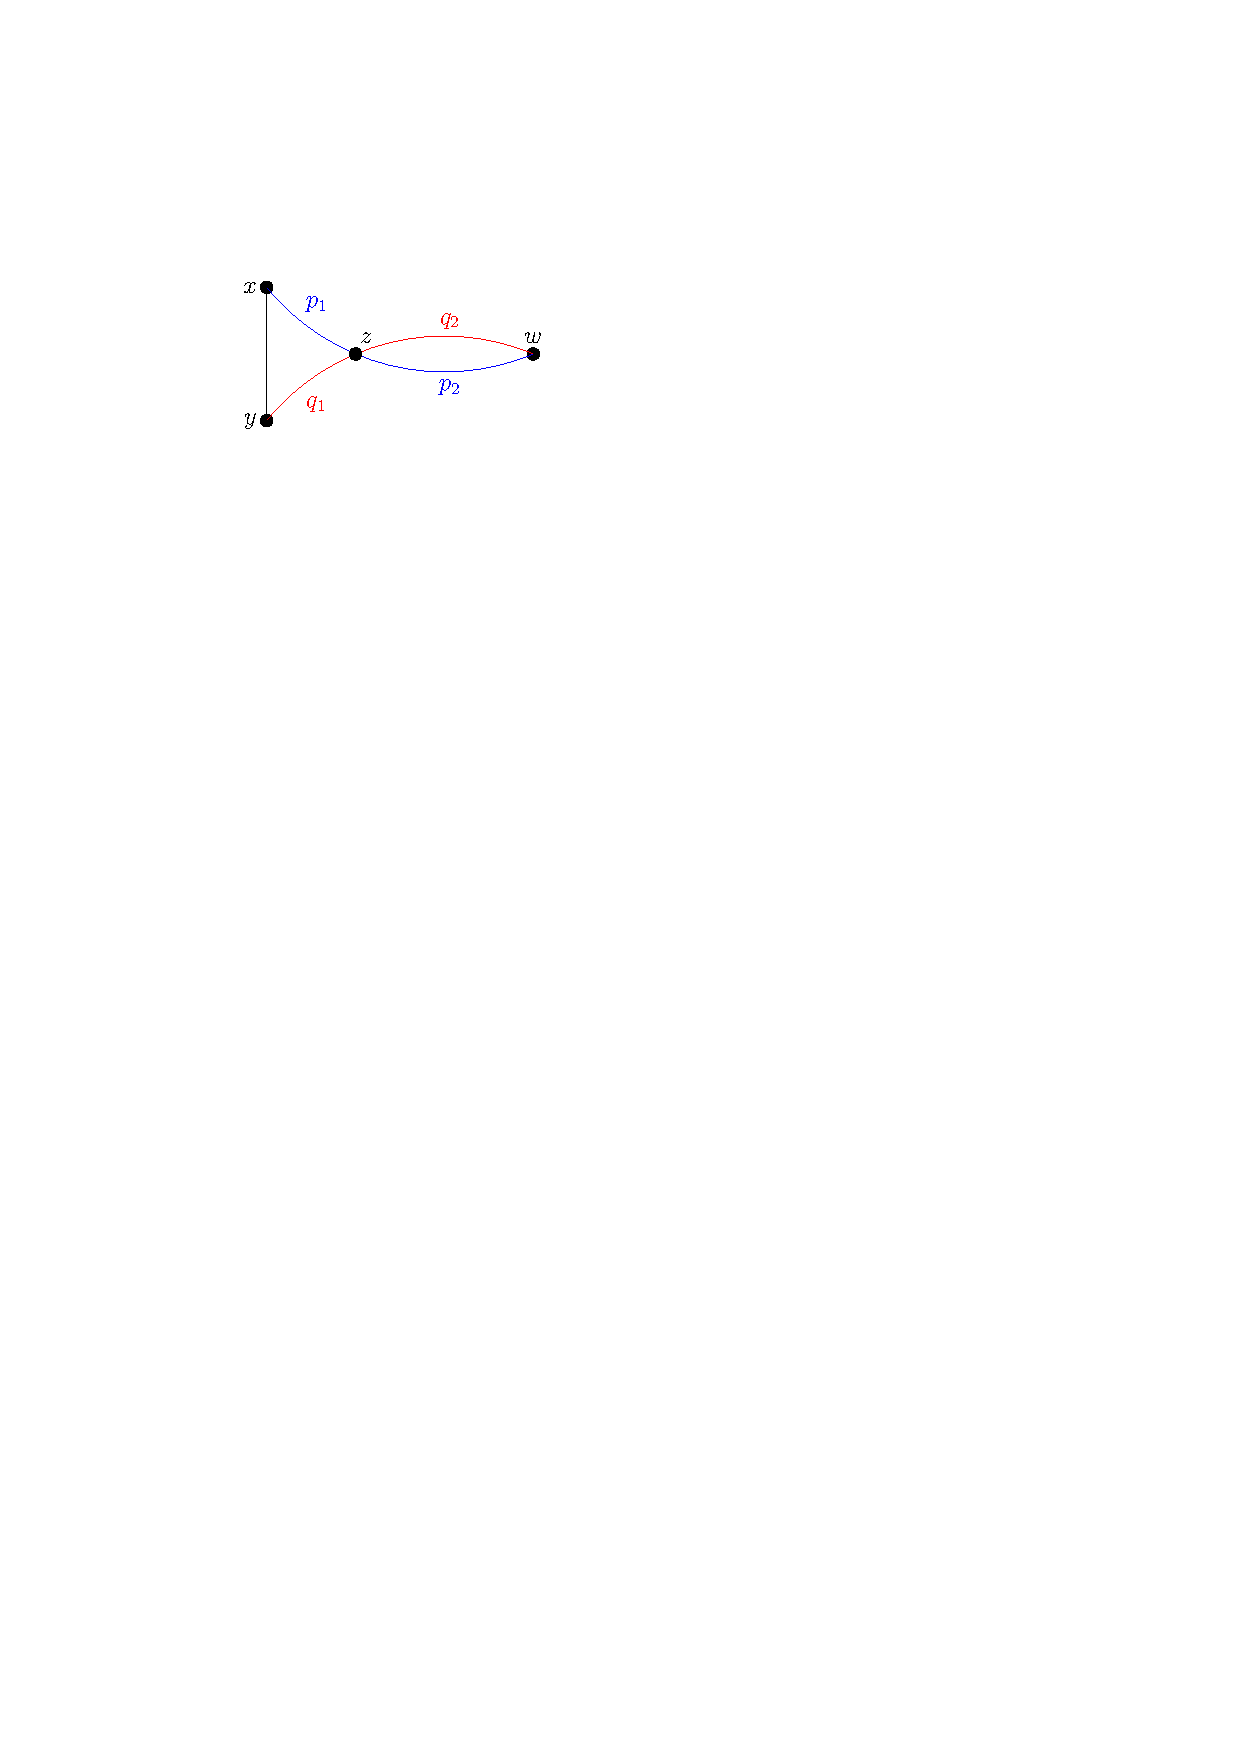
\includegraphics[width=0.3\linewidth]{figures/odd-length-cycle-bipartite.pdf}
        \caption{$p$ is the shortest path from $x$ to $w$. $q$ is the shortest path from $y$ to $w$. $p_1$ is the part of $p$ from $x$ to the last common vertex of $p$ and $q$. Similarly, $q_1$ is the part of $q$ from $y$ to the last common vertex of $p$ and $q$.}
        \label{fig:odd-length-cycle-bipartite}
    \end{figure}
    
    Let $p_1 = x \leadsto_p z$ be the part of the path $p$ from $x$ to $z$. Similarly, let $p_2 = z \leadsto_p w$, $q_1 = y \leadsto_q z$, and $q_2 = z \leadsto_q w$. We claim that $|p_2| = |q_2|$ since otherwise we can obtain a shorter path from $x$ to $w$ or from $y$ to $w$. Further, we claim that $|p_1|$ and $|q_1|$ have the same parity becuase $|p|$ and $|q|$ have the same parity and the second part of both paths, $p_2$ and $q_2$, are of the same length. Recall that $\{x,y\} \in E$. Then, $C = x \leadsto_{p_1} z \leadsto_{q_1} y \to x$. Since $|p_1|$ and $|q_1|$ have the parity, $|C| = |p_1| + |q_1| + 1$ is odd. This is becuase $|p_1| + |q_1|$ can be expressed as $2k$ for some $k \in \Z$. This is an odd-length cycle, which is a contradiction to our initial assumption that $G$ has no odd cycle. The only additional assumption leading to this contradiction is that $G$ is not bipartite. Hence, $G$ must be bipartite.
\end{proof}

\subsection{Coloring}

\begin{definition}[Proper Coloring]
    Let $G = (V,E)$ be a graph. A (proper) \textit{\textbf{coloring}} of $G$ is a function $\phi:\; V \to [k]$ such that for all $i \in [k]$, $\phi^{-1}(i)$ is independent. Equivalently, $\phi$ is a (proper) coloring of $G$ iff $\forall \{a,b\} \in E.\, \phi(a) \neq \phi(b)$. We call $\phi$ a $k$-coloring.
\end{definition}

\begin{definition}[Chromatic Number]
    The \textit{\textbf{chromatic number}} of a graph $G$, is the smallest $k$ such that there is a proper $k$ coloring of $G$. The chromatic number of $G$ is denoted by $\chi(G)$.
\end{definition}

\begin{theorem}
    A graph is 2-colorable if and only if it does not contain an odd-length cycle.
\end{theorem}

\begin{proof}
    Theorem \ref{thm:odd-length-cycle-bipartite} states that a graph is bipartite iff there is no odd-length cycle. To prove this theorem, it suffices to prove that a graph is 2-colorable if and only if the graph is bipartite.

    ($\implies$): Let $G = (V,E)$ be a 2-colorable graph. Take the coloring. Assign vertices with one color to $V_1$ and vertices with another color to $V_2$. $V_1$ and $V_2$ is a partition of $V$. By definition of a 2-color, for all $x,y \in V_1$, $\{x,y\} \not\in E$ and for all $x,y \in V_2$, $\{x,y\} \not\in E$.

    ($\impliedby$): Let $G=(V,E)$ be a bipartite graph where $V = V_1 \cup V_2$ is a partition. Assign one color to all vertices in $V_1$ and assign another color to all vertices in $V_2$. It is easy to prove that this is a valid 2-coloring directly from the definition of a bipartite graph.
\end{proof}

To demonstrate the concept of graph coloring and chromatic number, we consider the Petersen graph.

\begin{figure}[htbp]
    \centering
    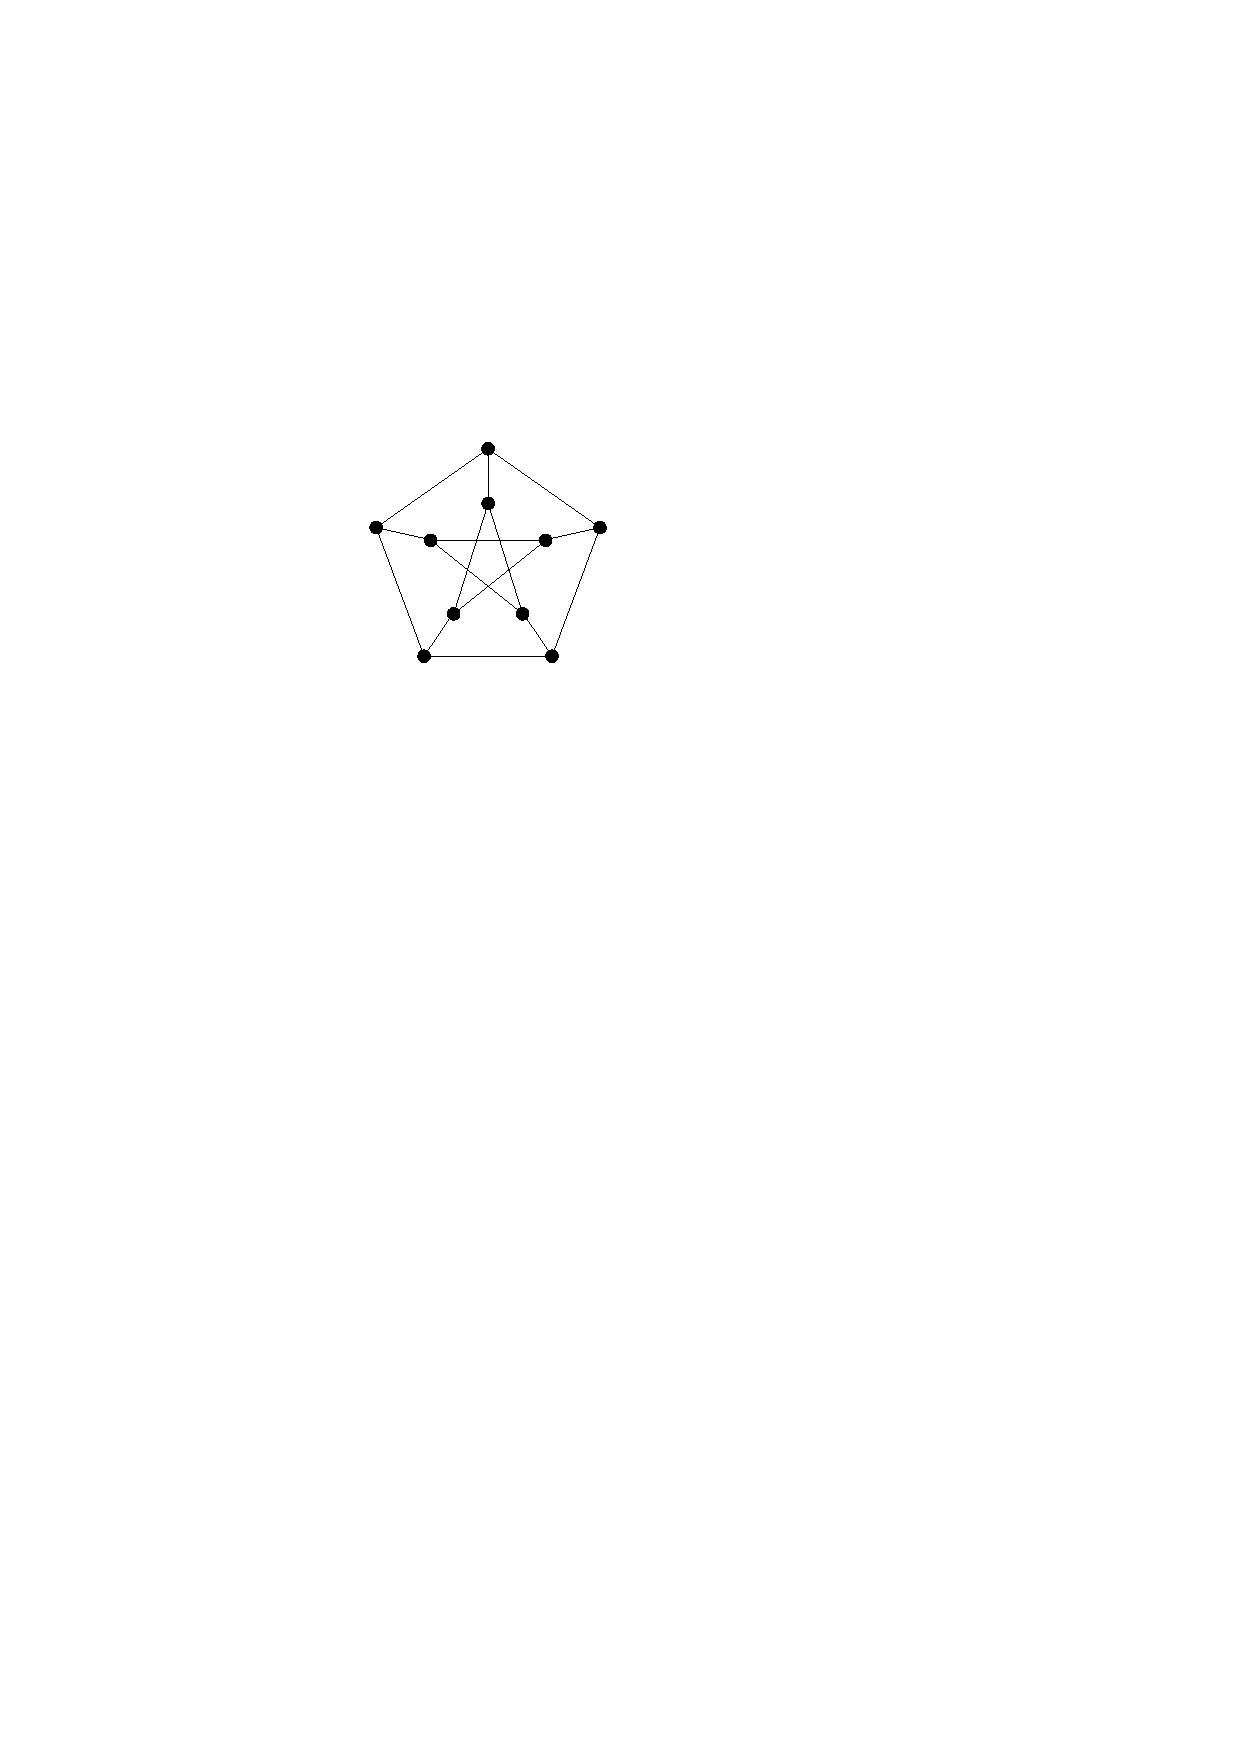
\includegraphics[width=0.2\linewidth]{figures/peterson-graph.pdf}
    \caption{The Petersen graph.}
    \label{fig:petersen-graph}
\end{figure}

\chapter{Planrity and Euler's Formula}
\section{Planarity}

\begin{definition}[Planarity]
    We say a graph $G$ is \textit{\textbf{planar}} if there \textbf{exists} a depiction of it on a plane without any edge crossing.
\end{definition}

To put in simple terms, a graph is planar if one can draw the graph on a piece of paper without any edge crossing each other. The definition as it is presented here is quite vague and lack mathematical rigor. Thankfully, this is formalized with a theorem by Kuratowski that we will introduce later that presents an equivalence to our definition of planarity.

There are many practical applications of graph planarity. In computer science, there is a notion of thickness that correlates planarity to how difficult it is to embed a network. Planarity is also related to integrated circuit design in cases when lines or wires are not allowed to cross.

\begin{theorem}[Four Color Theorem]
    Every planar graph has chromatic number of at most 4.
\end{theorem}

The proof of the Four Color theorem relies on brute-force computation methods and was only completed 1976. It is complex and not very readable, so we will not provide the proof here but instead treat it as a proven fact.

The Four Color Theorem implies that if $G$ is planar, $\chi(G) \leq 4$, so any graph with $\chi(G) \geq 5$ cannot be planar.

\begin{corollary}
    Any graph containing a copy of $K_5$ cannot be planar.
\end{corollary}

\subsection{Face}

Roughly speaking, a \textit{\textbf{face}} (in context of graph theory) is a region not containing other vertices or edges, bounded by edges of a graph in its planar depiction. Note that when discussing the \textbf{number of faces}, it is important to only consider the \textbf{planar depiction} of a graph because otherwise we can create arbitrary many faces.

\begin{figure}[htbp]
    \centering
    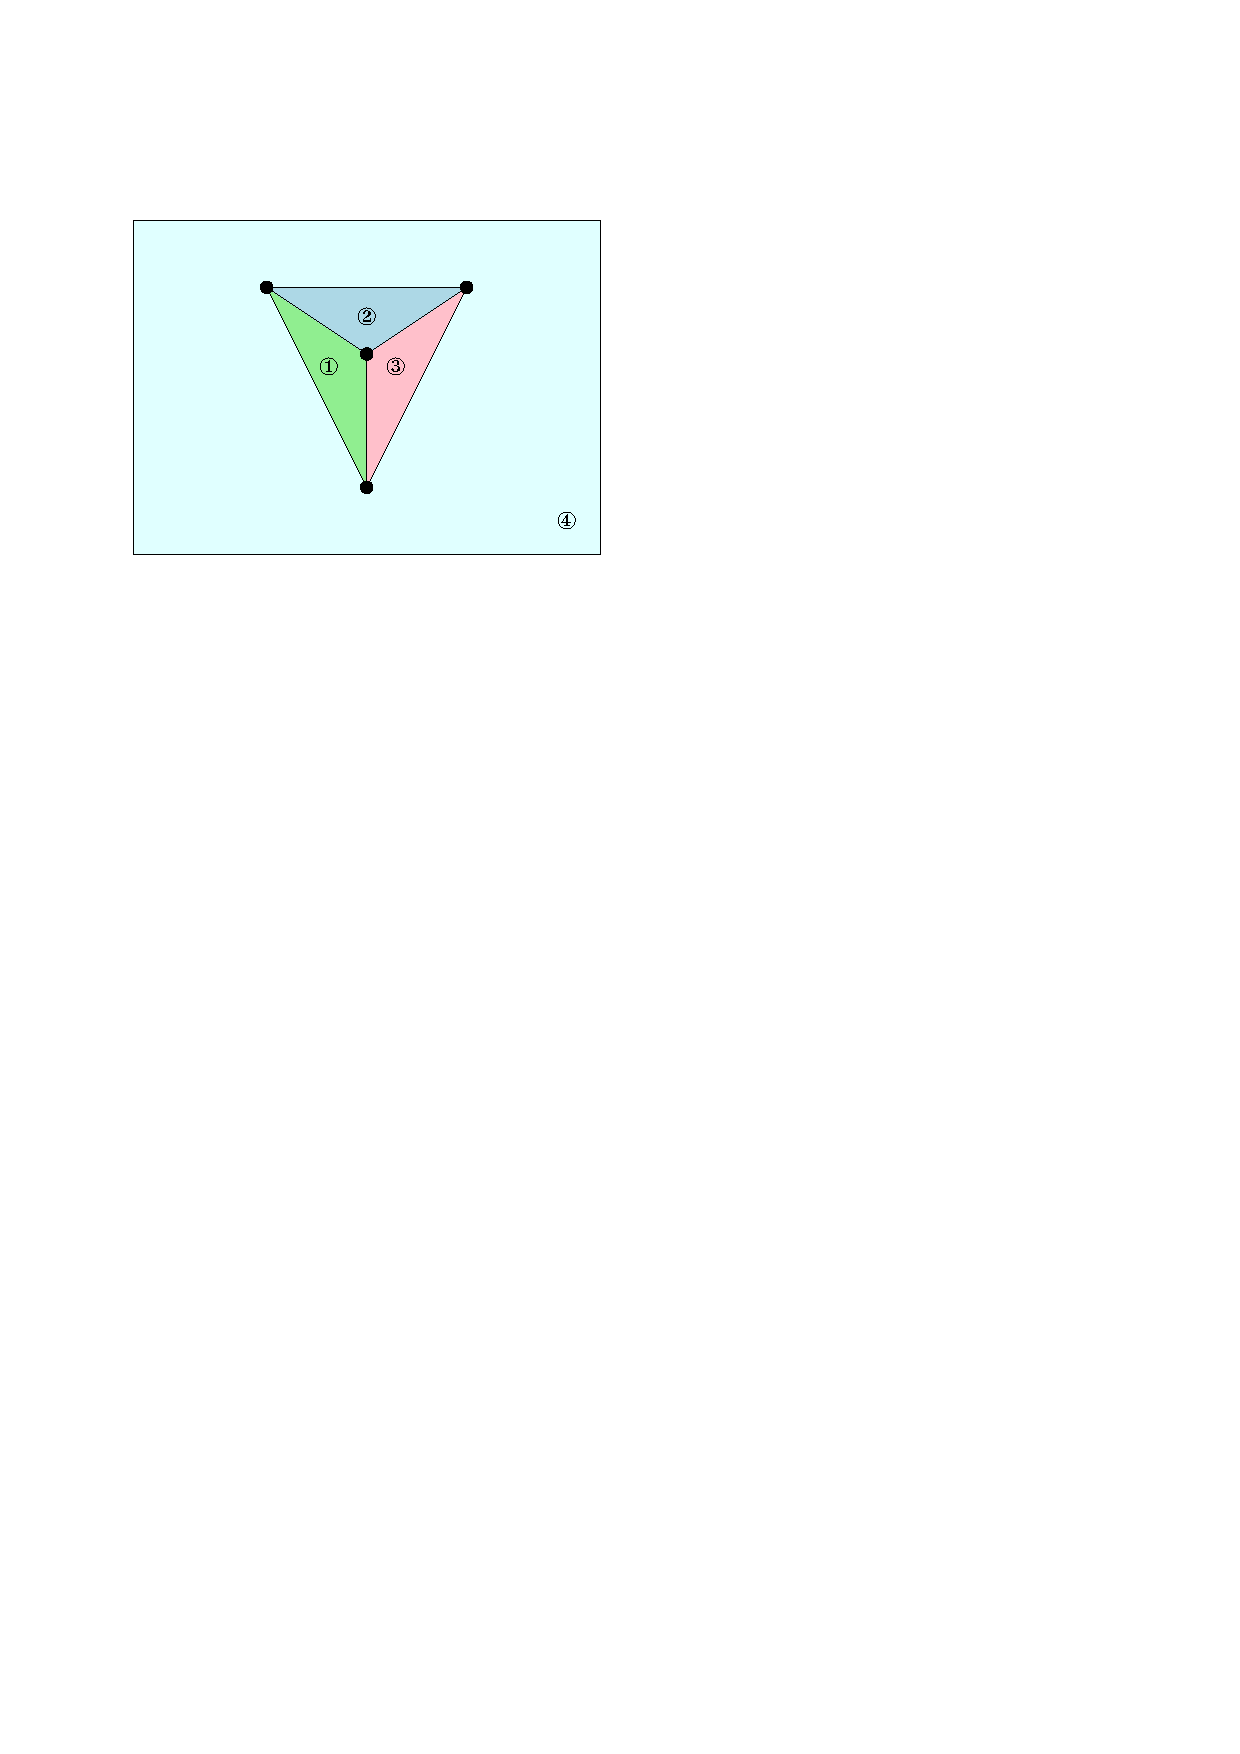
\includegraphics[width=0.4\linewidth]{figures/planar-graph-faces.pdf}
    \caption{A planar graph and its 4 faces.}
    \label{fig:planar-graph-faces}
\end{figure}

Is there any pattern between the number of vertices, edges, and faces in a planar graph? Consider the graph shown in Figure \ref{fig:planar-graph-faces}. We have 4 edges, 6 vertices, and 4 faces.

The triangle graph $K_3$ (complete graph of 3 vertices) has 3 vertices, 3 edges, and 2 faces. The path graph of $n$ vertices $P_n$ have $n$ vertices, $n-1$ edges, and one face. The cycle graph of $n$ vertices $C_n$ has $n$ vertices, $n$ edges, and 2 faces. See Figure \ref{fig:euler-formula-example-graphs}

\begin{figure}[htbp]
    \centering
    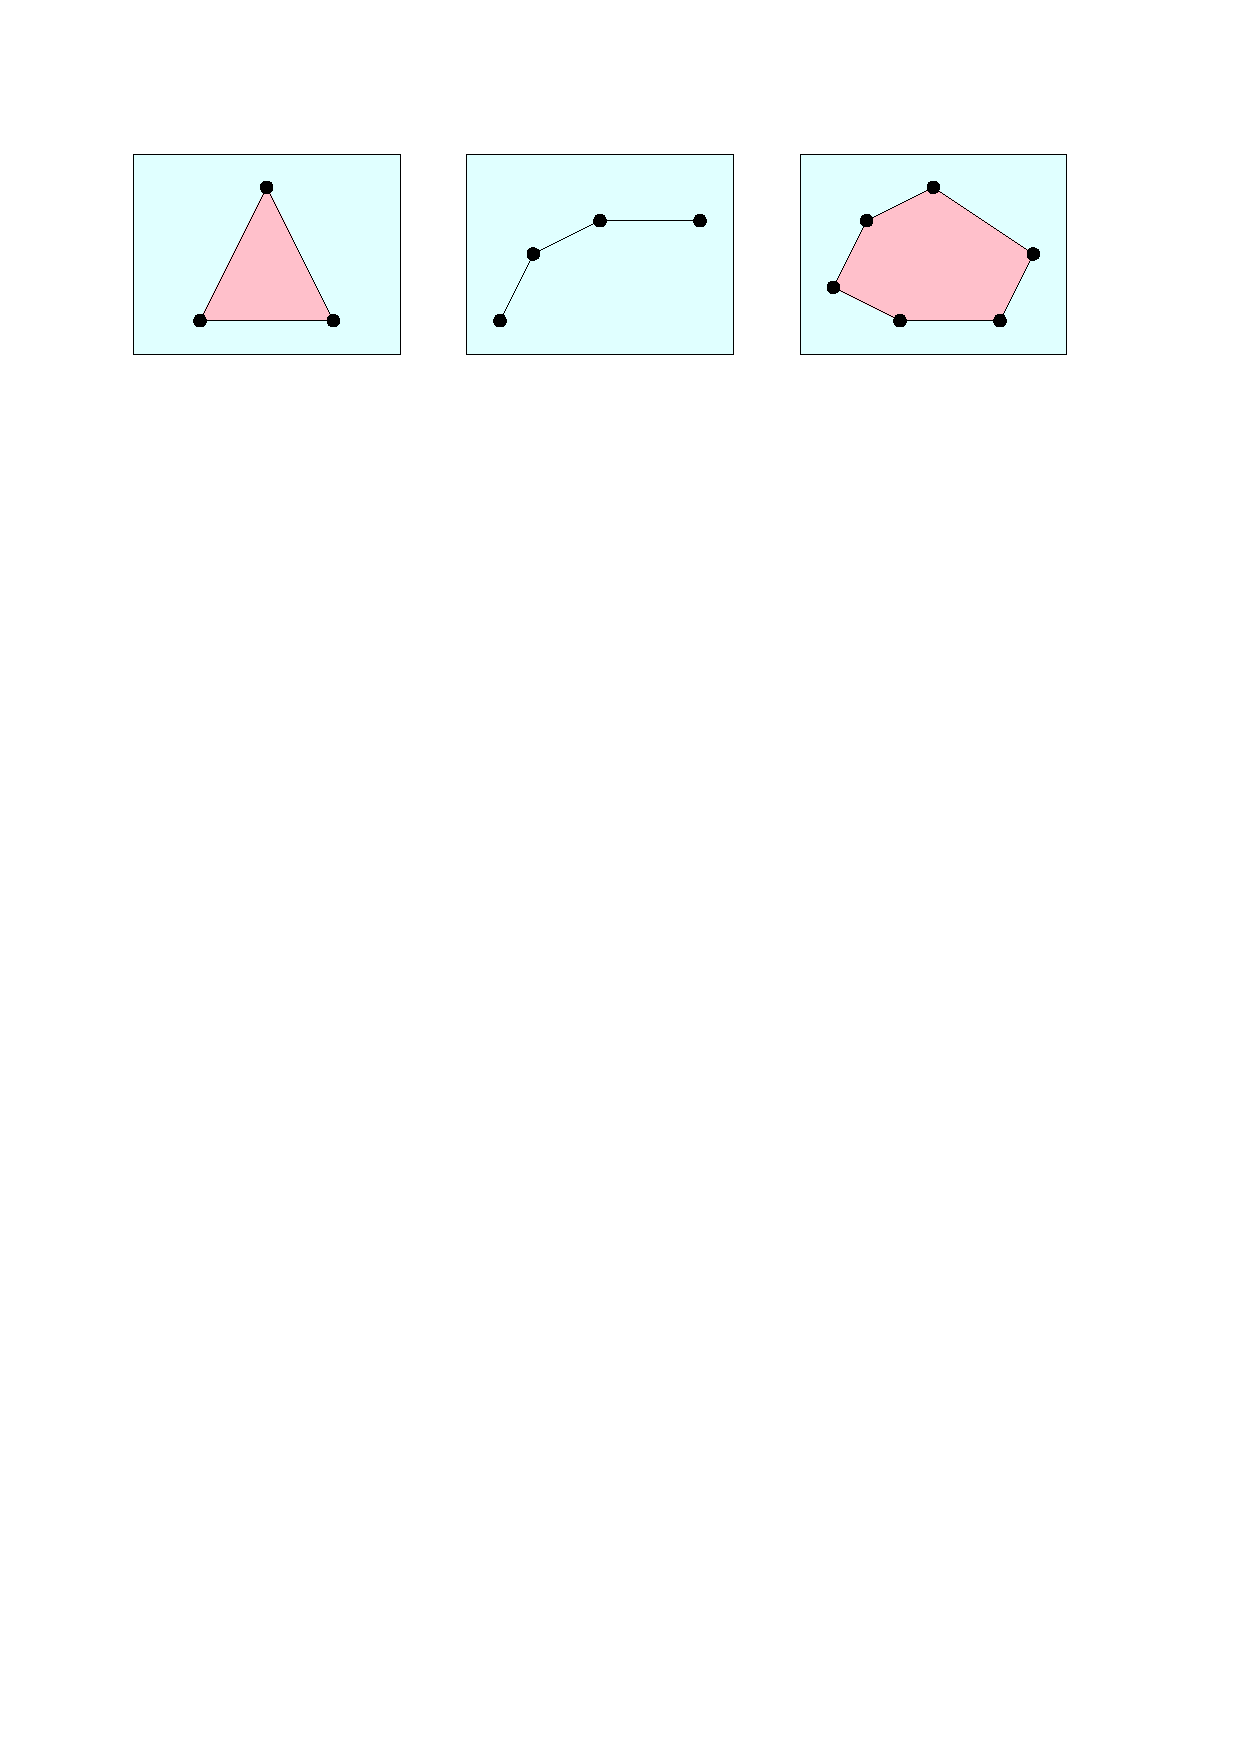
\includegraphics[width=0.6\linewidth]{figures/euler-formula-example-graphs.pdf}
    \caption{The triangle graph $K_3$, path graph $P_n$, and cycle graph $C_n$.}
    \label{fig:euler-formula-example-graphs}
\end{figure}

\section{Euler's Formula}

From the previous examples (Figure \ref{fig:planar-graph-faces} and \ref{fig:euler-formula-example-graphs}), we know there is some relationship between the number of vertices, edges, and faces in a planar depiction of a graph. This pattern is characterized by Euler's formula:

\begin{theorem}[Euler's Formula for Planar Graphs]
    Let $G$ be a connected planar graph with $n$ vertices, $m$ edges, and $f$ faces. Then,
    $$
    n - m + f = 2
    $$
\end{theorem}

\begin{proof}
    By induction on $m$.

    \textbf{Base Case}: When $m = 0$. $G$ is connected, so graph is a singleton vertex. It has one face. And clearly, $1 - 0 + 1 = 2$.

    \textbf{Inductive Step}: Let $m \in \N \cup \{0\}$ be arbitrary. Assume that Euler's formula holds for graphs with $m$ edges. Let $G$ be a graph with $m+1$ edges.
    
    Case 1: If we can remove an edge so that the graph is still connected, then the edge being removed must divide some face into two. Let $G'$ be the graph after removing the edge. Removing the edge does not change the number of vertices, so $G'$ has $n$ vertices, $m$ edges, and $f$. By inductive hypothesis,
    $$
    n - m + f = 2
    $$
    After adding the edge back, we have $m+1$ edges and $f+1$ since the edge divides a face into two so adding it back adds one more face. Hence, in $G$, we have
    $$
    n - (m+1) + (f+1) = m - m + f = 2
    $$
    In this case, Euler's formula holds for $G$ with $m+1$.

    Case 2: If removing any edge leaves the graph disconnected, the graph must be a tree. Tree has 1 face, and $n = m + 1$. So, for $G$,
    $$
    n - m + f = m + 1 - m + f = 2
    $$
    Euler's formula also holds for this case.

    By induction, Euler's formula holds for all graphs.
\end{proof}

\subsection{A Useful Corollary}

A useful corollary about planar graphs follows from Euler's formula.

\begin{corollary}
    Let $G$ be a planar graph with $n \geq 3$ vertices and $m$ edges. Then,
    $$
    m \leq 3n - 6
    $$
\end{corollary}

\begin{proof}
    We consider two cases: $G$ is connected and $G$ is disconnected.

    Case 1: $G$ is connected. We can assume that $G$ is not a tree since the case where $G$ is a tree is trivial. Let $S$ be the set of pairs $(e,F)$ where $e$ is an edge and $F$ is a face such that $e$ \textbf{is an edge on the face} $F$. For a fixed $e$,
    $$
    |\{F \mid (e,F) \in S\}| \leq 2
    $$
    as an edge borders at most two faces.

    For a fixed $F$,
    $$
    |\{e \mid (e,F) \in S\}| \geq 3 
    $$
    since an enclosed area must have at least three boundaries. Then it follows that $3f \leq |S| \leq 2m$. By Euler's formula,
    $$
    m = n + f - 2 \leq n + \frac{2}{3}m - 2 \implies m \leq 3n - 6
    $$

    Case 2: $G$ is disconnected. Consider each connected component of $G$. Use the same argument as Case 1 to conclude that the inequality holds for each connected components and thus must hold for the entire graph.
\end{proof}

\section{Graph Minor and Contraction}

\begin{definition}[Contraction]
    Let $G = (V,E)$ be a graph and let $e \in E$ be an edge. A \textit{\textbf{contraction}} along $e$ is a graph $G' = ((V \setminus e) \cup \{e\}, E')$ where $E'$ is defined such that for all $u,v \in (V \setminus e)$,
    $$
    \{u,v\} \in E \iff \{u,v\} \in E'
    $$
    and
    $$
    \{u,e\} \in E' \iff \exists x \in e.\, \{u,x\} \in E.
    $$
\end{definition}

\begin{definition}[Graph Minor]
    A \textit{\textbf{graph minor}} of a graph $G$ is a graph $H$ obtained via a process of taking subgraphs and contractions.
\end{definition}

We are interested in graph minor because it gives us an important equivalent characterization for planar graphs.

\begin{theorem}[Kuratowski, 1930]
    A graph is planar if and only if it does not contain $K_5$ or $K_{3,3}$ as a minor.
\end{theorem}

\begin{theorem}[Wagner, 1937]
    A graph is planar if and only if it has no minor isomorphic to $K_3$ or $K_{3,3}$.
\end{theorem}

\subsection{Application of Kuratowski's Theorem}

We use Kuratowski's theorem to show that Petersen's graph is not planar.

\begin{figure}[htbp]
    \centering
    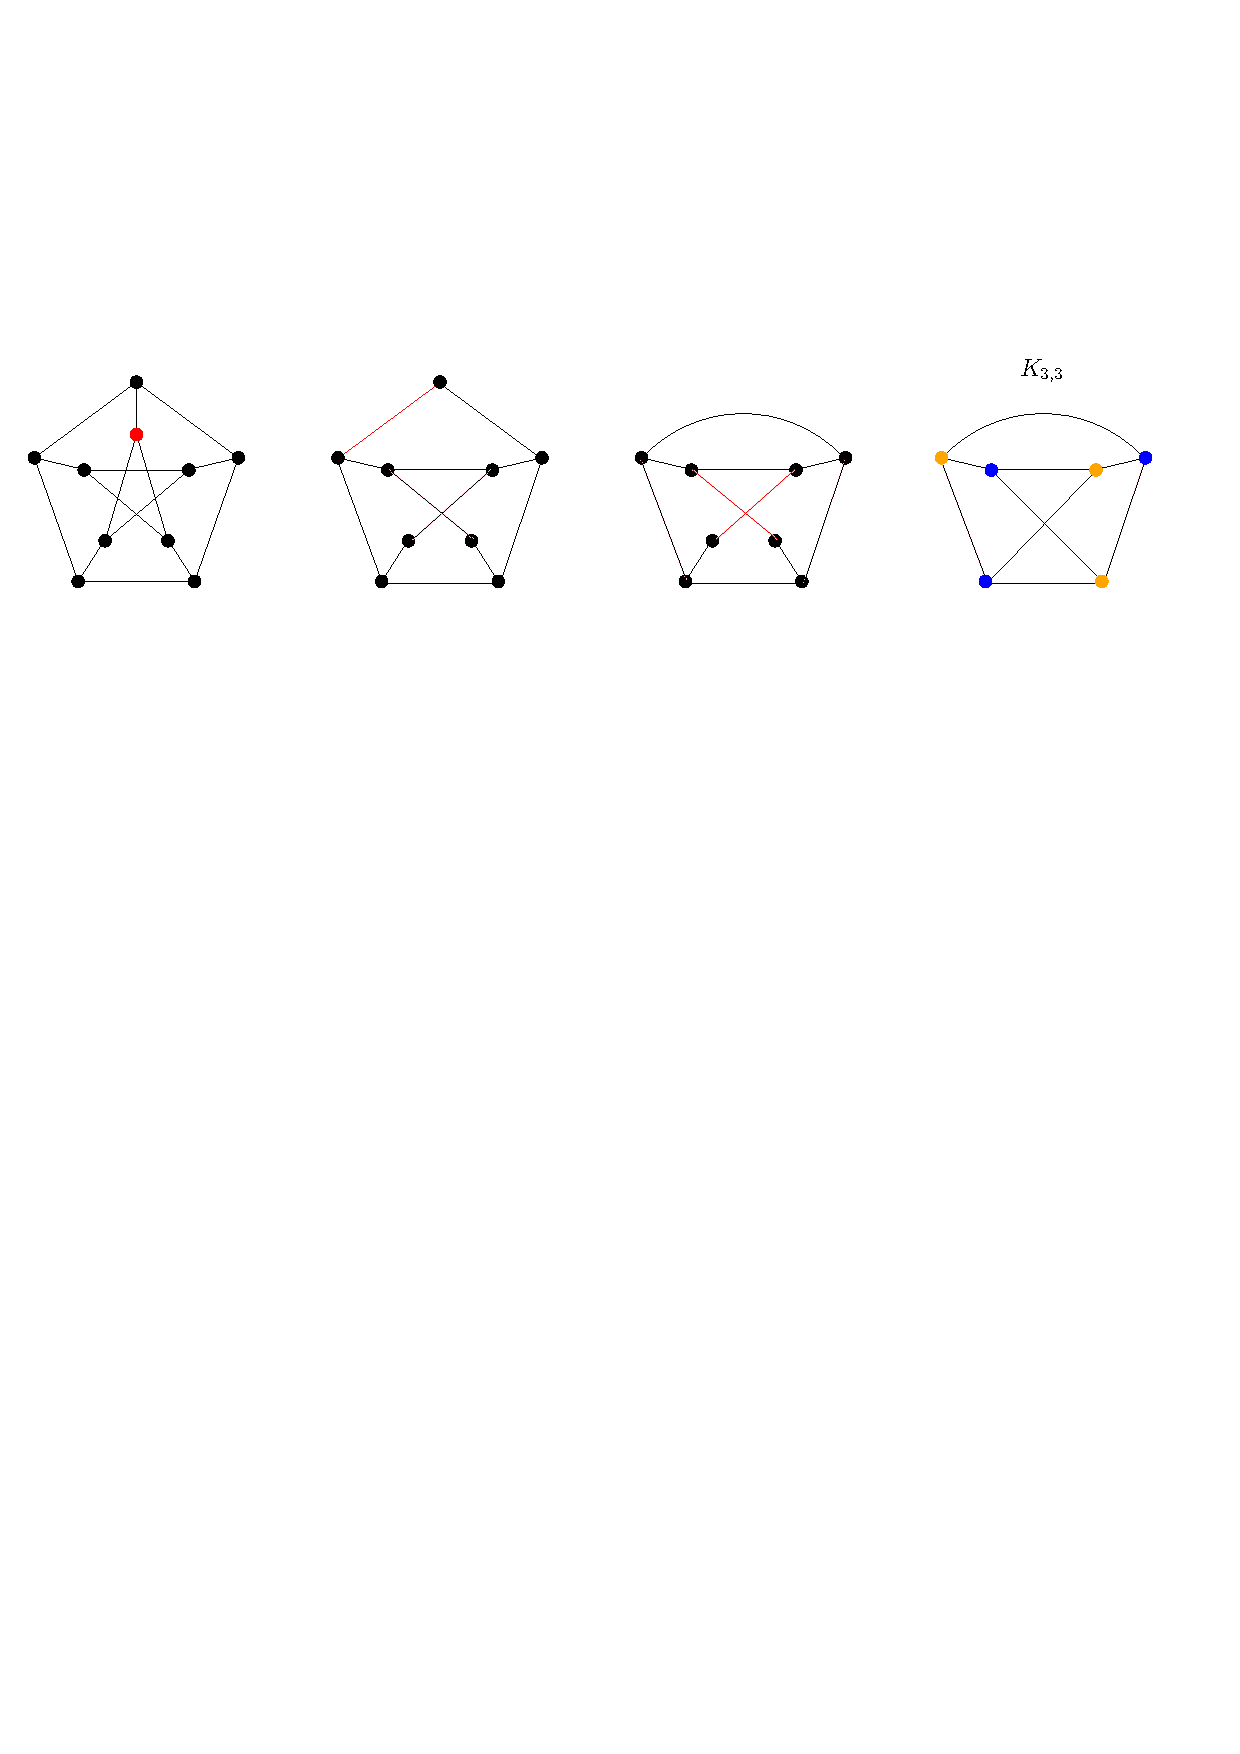
\includegraphics[width=0.9\linewidth]{figures/petersen-graph-nonplanar.pdf}
    \caption{First, take the subgraph by removing the red vertex and edges connected to it. Then, contract the red edges. We notice that after these steps, we get a graph minor that is isomorphic to $K_{3,3}$.}
    \label{fig:petersen-graph-nonplanar}
\end{figure}

\section{Formalizing Planrity Using Topology (not covered in class)}

\chapter{Counting Trees}
\section{Counting Trees}

Recall that a tree is a connected graph with the property that any two vertices are connected by a unique path. Equivalently, a tree is a connected graph with $n-1$ edges and $n$ vertices. A tree with at least $n \geq 2$ vertices has at least two vertices of degree one (the leaves).

\begin{definition}[Labeled Tree]
    A \textit{\textbf{labeled tree}} is a tree $T$ whose vertex set is $\{1,\ldots,n\}$.
\end{definition}

We would like to \textbf{count} how many possible $E$ exist such that $([n], E)$ forms a \textbf{labeled tree}. We are not counting isomorphisms here so the labels matter. To answer this question, we introduce \textbf{Pr\"ufer's cod}e, which transforms trees into strings that are easy to count.

\subsection{Pr\"ufer Code}

Fix $n \geq 2$. Let $s:\; [n-2] \to \{1,\ldots,n\}$ be a sequence (string over $\{1,\ldots,n\}$ of length $n-1$). Consider the following algorithm that generates a set $E$ of size $n-2$.
\begin{codebox}
    \Procname{$\proc{Prufer-Decode}(s)$}
    \li $L = \{1,\ldots,n\}$
    \li \While $|s| > 0$ \Do
        \li find the smallest $j$ that is not in $s$, add $\{j,s[1]\}$ to $E$
        \li set $L = L \setminus \{j\}$
        \li delete $s[1]$
    \End
    \li set $E = E \cup \{L\}$
    \li \Return $E$
\end{codebox}
The algorithm above assigns to each sequence $s$, a set $E$ of size $n-1$ such that $([n], E)$ is connected.

\begin{figure}[htbp]
    \centering
    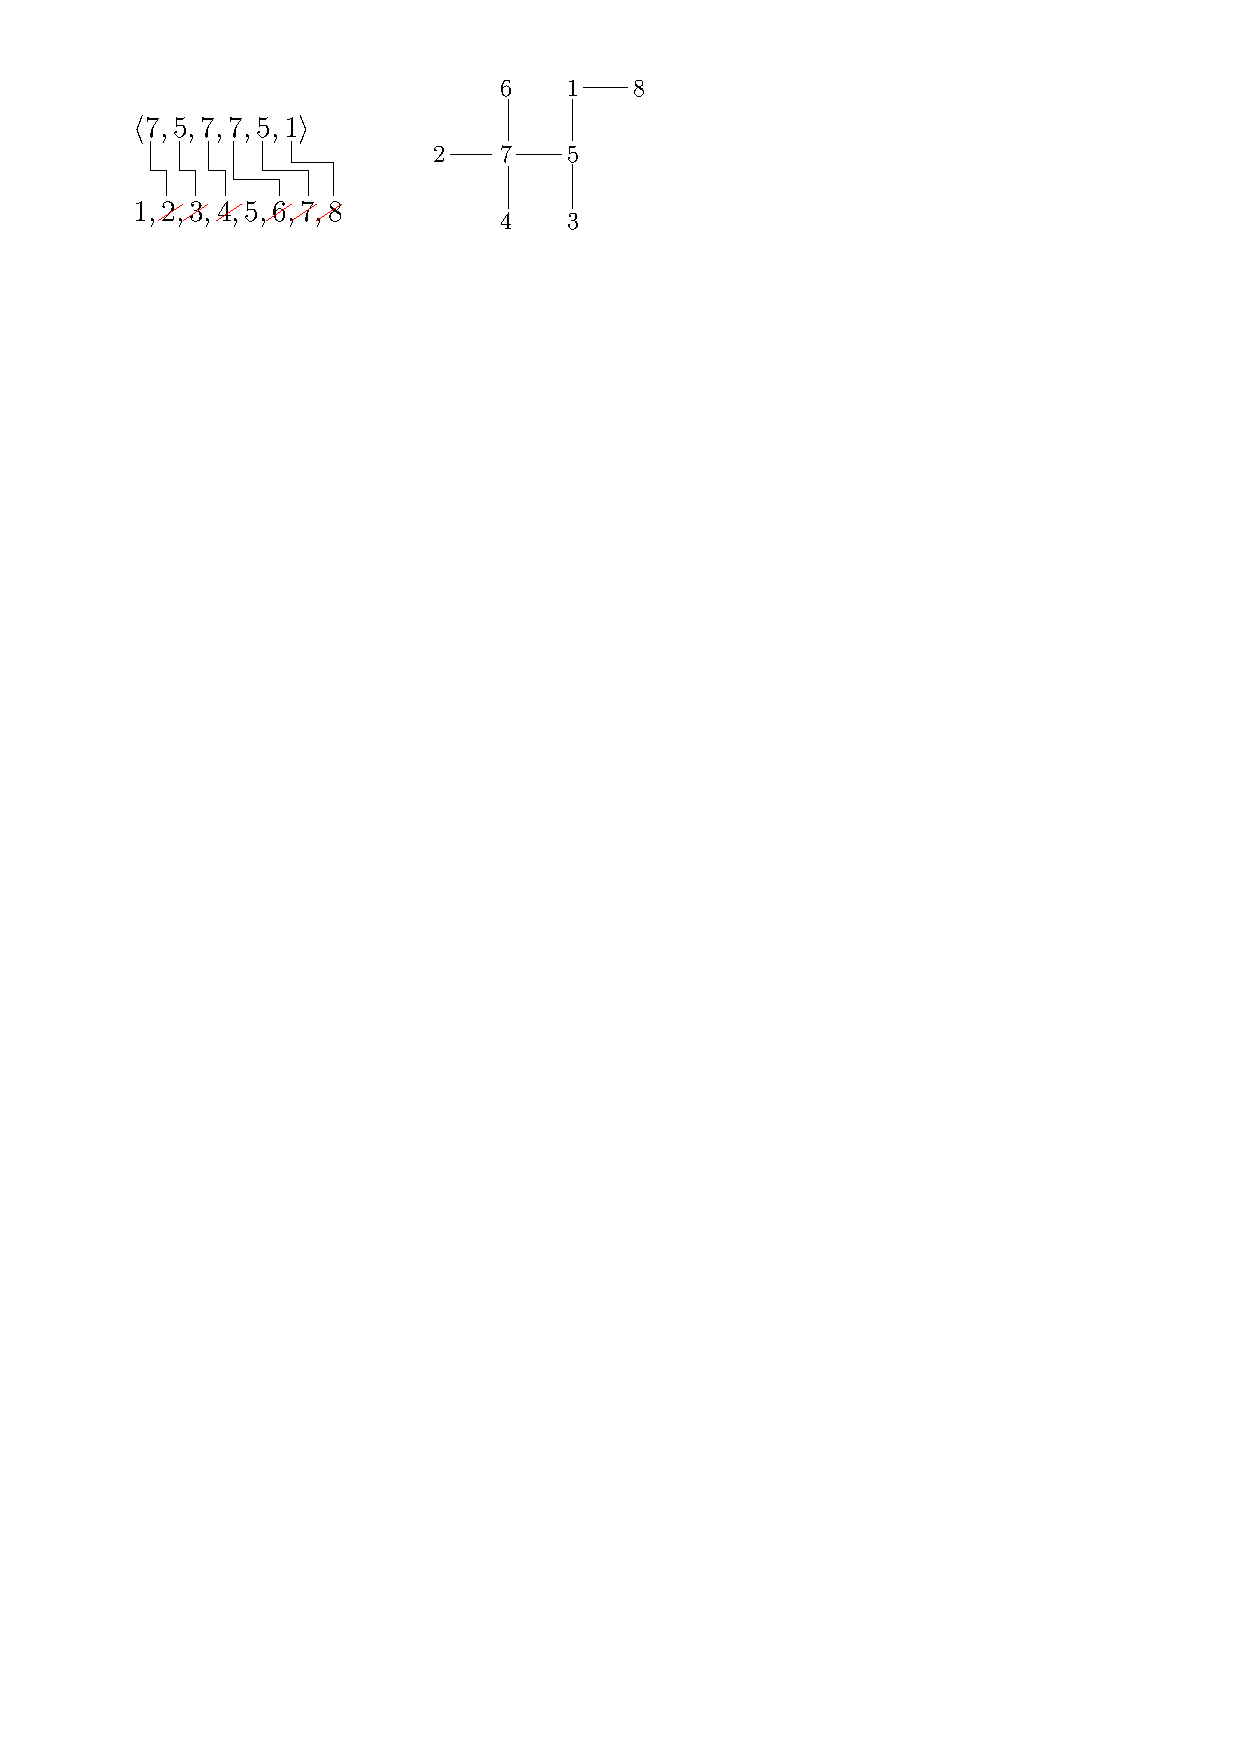
\includegraphics[width=0.5\linewidth]{figures/prufer-code-example.pdf}
    \caption{Example of a tree and its corresponding Prufer code}
    \label{fig:prufer-code-example}
\end{figure}

We can reverse the algorithm above to encode a tree into its Pr\"ufer code.

\begin{codebox}
    \Procname{$\proc{Prufer-Encode}(E)$}
    \li \For $i = 1$ \To $n-2$ \Do
        \li $s[i]$ = the unique vertex adjacent to the leaf with the smallest value
        \li remove the leaf with the smallest value
    \End
    \li \Return $s$
\end{codebox}

\subsection{Back to Counting Trees}

Each labeled tree with $n$ vertices has a unique Pr\"ufer's code of length $n-2$. Then, counting the number of labeled trees is equivalent to counting the number of Pr\"ufer codes for all the trees.

\begin{theorem}[Cayley's Formula]
    For each $n \geq 2$, there are exactly $n^{n-2}$ labeled trees on $\{1,\ldots,n\}$.
\end{theorem}

\begin{proof}
    To each tree, find the unique associated Pr\"ufer code $s:\; [n-2] \to [n]$. This creates a bijective correspondence between labeled trees and sequences $s:\; [n-2] \to [n]$.

    There are exactly $n^{n-2}$ such sequences and hence that many labeled trees on $\{1,\ldots,n\}$.
\end{proof}

\part{Posets}

\chapter{Basic Definitions of Posets}
\section{Basic Definitions}

\begin{definition}[Poset (partially ordered set)]
    A \textit{\textbf{poset}} $\mathbb{P}$ is a pair $\mathbb{P} = (X,P)$ where $X$ is a set and $P \subseteq X \times X$ is a relation that is
    \begin{itemize}
        \item reflexive: $\forall a \in X.\, (a,a) \in P$
        \item anti-symmetric: $a \neq b \land (a,b) \in P \implies (b,a) \not\in P$
        \item transitive: $(a,b) \in P \land (b,c) \in P \implies (a,c) \in P$
    \end{itemize}
\end{definition}

Instead of writing $(a,b) \in P$, we use the notation $a \leq_{\mathbb{P}} b$.

\begin{definition}[Embedding, Isomorphism, Automorphism]
    Given a poset $\mathbb{P} = (X,P)$ and $\mathbb{Q} = (Y,Q)$, an \textbf{embedding} from $\mathbb{P}$ into $\mathbb{Q}$ is an injective map $f:\; X \to Y$ with the property that $a \leq_{\mathbb{P}} b$ if and only if $f(a) \leq_{\mathbb{Q}} f(b)$. If the embedding is surjective, we call it an \textbf{isomorphism}. If $\mathbb{Q} = \mathbb{P}$, we call it an \textbf{automorphism}.
\end{definition}

For example, consider $X = \{\star, \circ, \diamond \}$ with $P = \{ (\star,\star), (\circ,\circ), (\diamond, \diamond), (\diamond, \star) \}$, and $Y = \{\star, \circ, \diamond, \Box \}$ with $Q = \{ (\star,\star), (\circ,\circ), (\diamond,\diamond), (\Box,\Box), (\Box,\star) \}$. Let $\mathbb{P} = (X,P)$ and $\mathbb{Q} = (Y,Q)$. Consider the function $f:\; X \to Y$ such that $f(\star) = \star$, $f(\circ) = \circ$, and $f(\diamond) = \Box$. $f$ is an embedding because $\diamond \leq_{\mathbb{P}} \star$ if and only if $f(\diamond) = \Box \leq_{\mathbb{Q}} \star = f(\star)$. However, $f$ is not an isomorphism because $\diamond$ is not in the range of $f$ so $f$ is not surjective.

\begin{definition}[Dual]
    Given a poset $\mathbb{P} = (X,P)$, we call the poset $\mathbb{P}^d = (X,P^d)$ where $a \leq_{\mathbb{P}^d} b \iff b \leq_{\mathbb{P}_d} a$ the \textbf{dual} of $\mathbb{P}$. We say a poset is self-dual if it is isomorphic to its dual.
\end{definition}

\begin{definition}[Cover]
    Given a poset $\mathbb{P} = (X,P)$ and a point $a \in X$, we say $a$ is \textbf{covered by} a point $b \in X$ if $a <_{\mathbb{P}} b$ and there is no $c$ such that $a <_{\mathbb{P}} c <_{\mathbb{P}} b$.
\end{definition}

\begin{definition}[Cover Graph]
    Given a poset $\mathbb{P} = (X,P)$, we call the graph $G = (X,E)$ given by $\{x,y\} \in E$ if and only if $x$ covers $y$ or $y$ covers $x$, the \textbf{cover graph} associated to $\mathbb{P}$. 
\end{definition}

If we draw the cover graph in an oriented fashion where lower vertices correspond to the $\leq_{\mathbb{P}}$-smaller elements, we have a special kind of cover graph known as \textbf{Hasse diagram}.

Let $\mathbb{P} = (X,P)$ be a poset where $X = \{a,b,c,d,e,f\}$ and $P = \{ (a,c), (b,c), (b,d), (d,e), (a,e), (e,f)\}$. One possible cover graph and the Hasse diagram is shown below.

\begin{figure}[htbp]
    \centering
    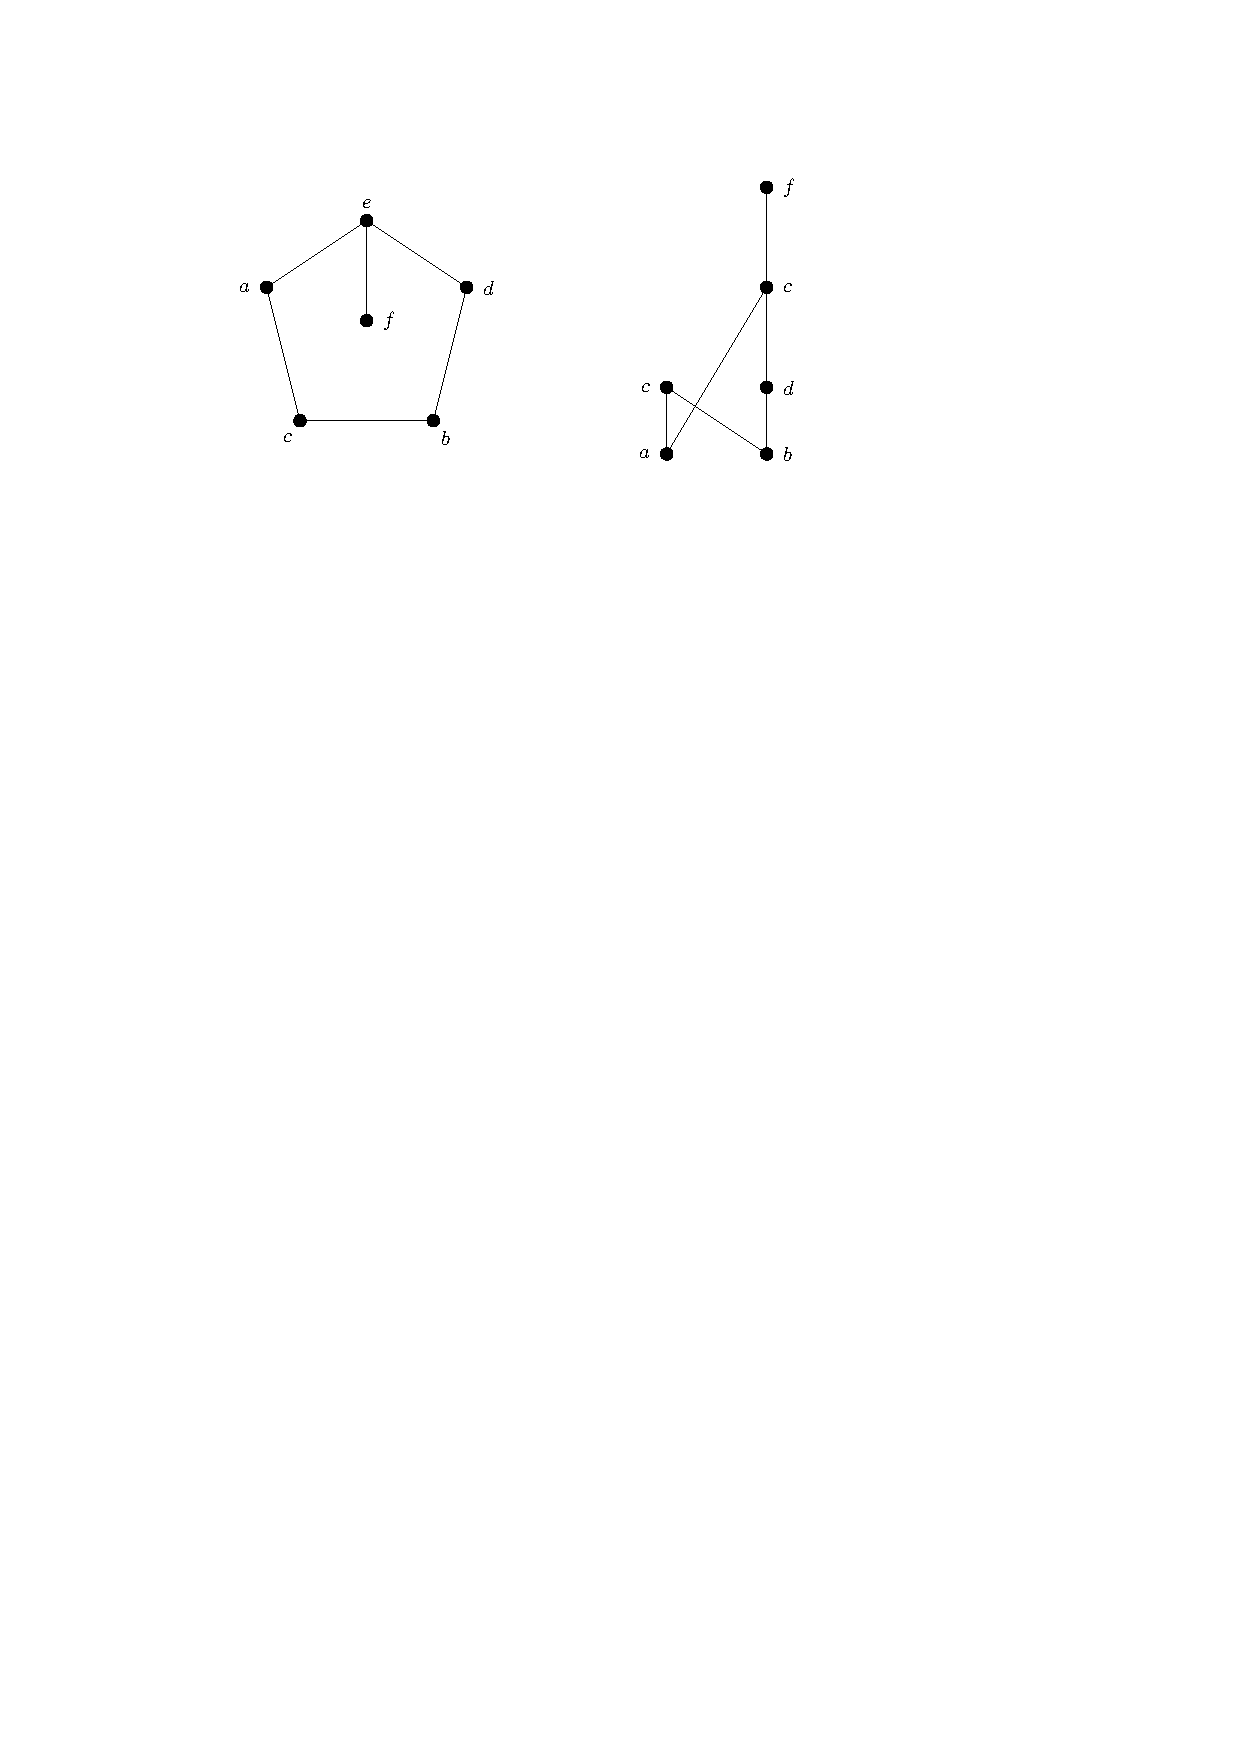
\includegraphics[width=0.5\linewidth]{figures/hasse-diagram.pdf}
    \caption{Cover graph and Hasse diagram for the poset described above.}
    \label{fig:hasse-diagram-example}
\end{figure}

\section{Linear Orders}

\begin{definition}[Comparability]
    Given a poset $\mathbb{P} = (X,P)$, we say two points $a,b \in X$ are \textit{\textbf{comparable}} if either $a <_{\mathbb{P}} b$ or $b <_{\mathbb{P}} b$ If two points are not comparable, we call them \textit{\textbf{incomparable}}.
\end{definition}

\begin{definition}[Total/Linear Order]
    Given a poset $\mathbb{P} = (X,P)$, we say $\mathbb{P}$ is \textit{\textbf{linearly ordered}} or \textit{\textbf{totally ordered}} if no two distinct points are incomparable.
\end{definition}

\section{Height and Width}

\begin{definition}[Antichain and Chain]
    Given a poset $\mathbb{P} = (X,P)$, we call $A \subseteq X$ an \textit{\textbf{antichain}} if every pair of distinct elements in $A$ are \textbf{incomparable}. We call a subset $C \subseteq X$ a \textit{\textbf{chain}} is every pair of distinct elements is \textbf{comparable}.
\end{definition}

\begin{definition}[Height and Width]
    Given a poset $\mathbb{P} = (X,P)$, we define the parameters $\mathsf{width}(\mathbb{P})$ and $\mathsf{height}(\mathbb{P})$ to denote the size of the largest antichain and chain of $\mathbb{P}$, respectively.
\end{definition}

\section{Subset Lattice and Sperner's Theorem}

\begin{theorem}[Sperner's Theorem]
    Consider the poset $\mathbb{P} = (\mathcal{P}([n]), \subseteq)$. Then, $\mathsf{width}(\mathbb{P}) = \binom{n}{\floor{n/2}}$.
\end{theorem}

\begin{proof}
    One can easily verify that $A = \{ S \subseteq [n] \mid |S| = \floor{\frac{n}{2}}\}$ is an \textbf{antichain}. Two sets of the same size are comparable if and only if they are equal. There are $\binom{n}{\floor{\frac{n}{2}}}$ such subsets of $[n]$ of size $\floor{\frac{n}{2}}$, so $\mathsf{width}(\mathbb{P}) \geq \binom{n}{\floor{\frac{n}{2}}}$. This shows that $\binom{n}{\floor{\frac{n}{2}}}$ is a lower bound.

    Now, we proceed to show that $\binom{n}{\floor{\frac{n}{2}}}$ is also an upper bound. Let $A = \{ S_1, \ldots, S_w \}$ be a \textbf{maximal antichain} of $\mathbb{P}$. It suffices to show that $w \leq \binom{n}{\floor{\frac{n}{2}}}$. For each $S_i \in A$, let $\mathcal{C}_i$ be the set of all \textbf{maximal chains} that contains $S_i$. We note that a maximal chain but be an $\subseteq$-increasing sequences that differs by at most one element per successive cover. If the next subset in the chain \textbf{differs} from the previous subset \textbf{by more than one element}, then the chain \textbf{would not be maximal}. In other words, starting from $S_i$, we remove 1 element until we reaches the empty set, and add 1 element until we reaches $[n]$. There are $|S_i|!$ ways to remove points successively from $S_i$. Similarly, there are $(k-|S_i|)!$ ways to add points successively to $S_i$. Therefore, for any $i$, $|\mathcal{C}_i| = |S_i|! \cdot (k-|S_i|)!$.

    \begin{figure}[htbp]
        \centering
        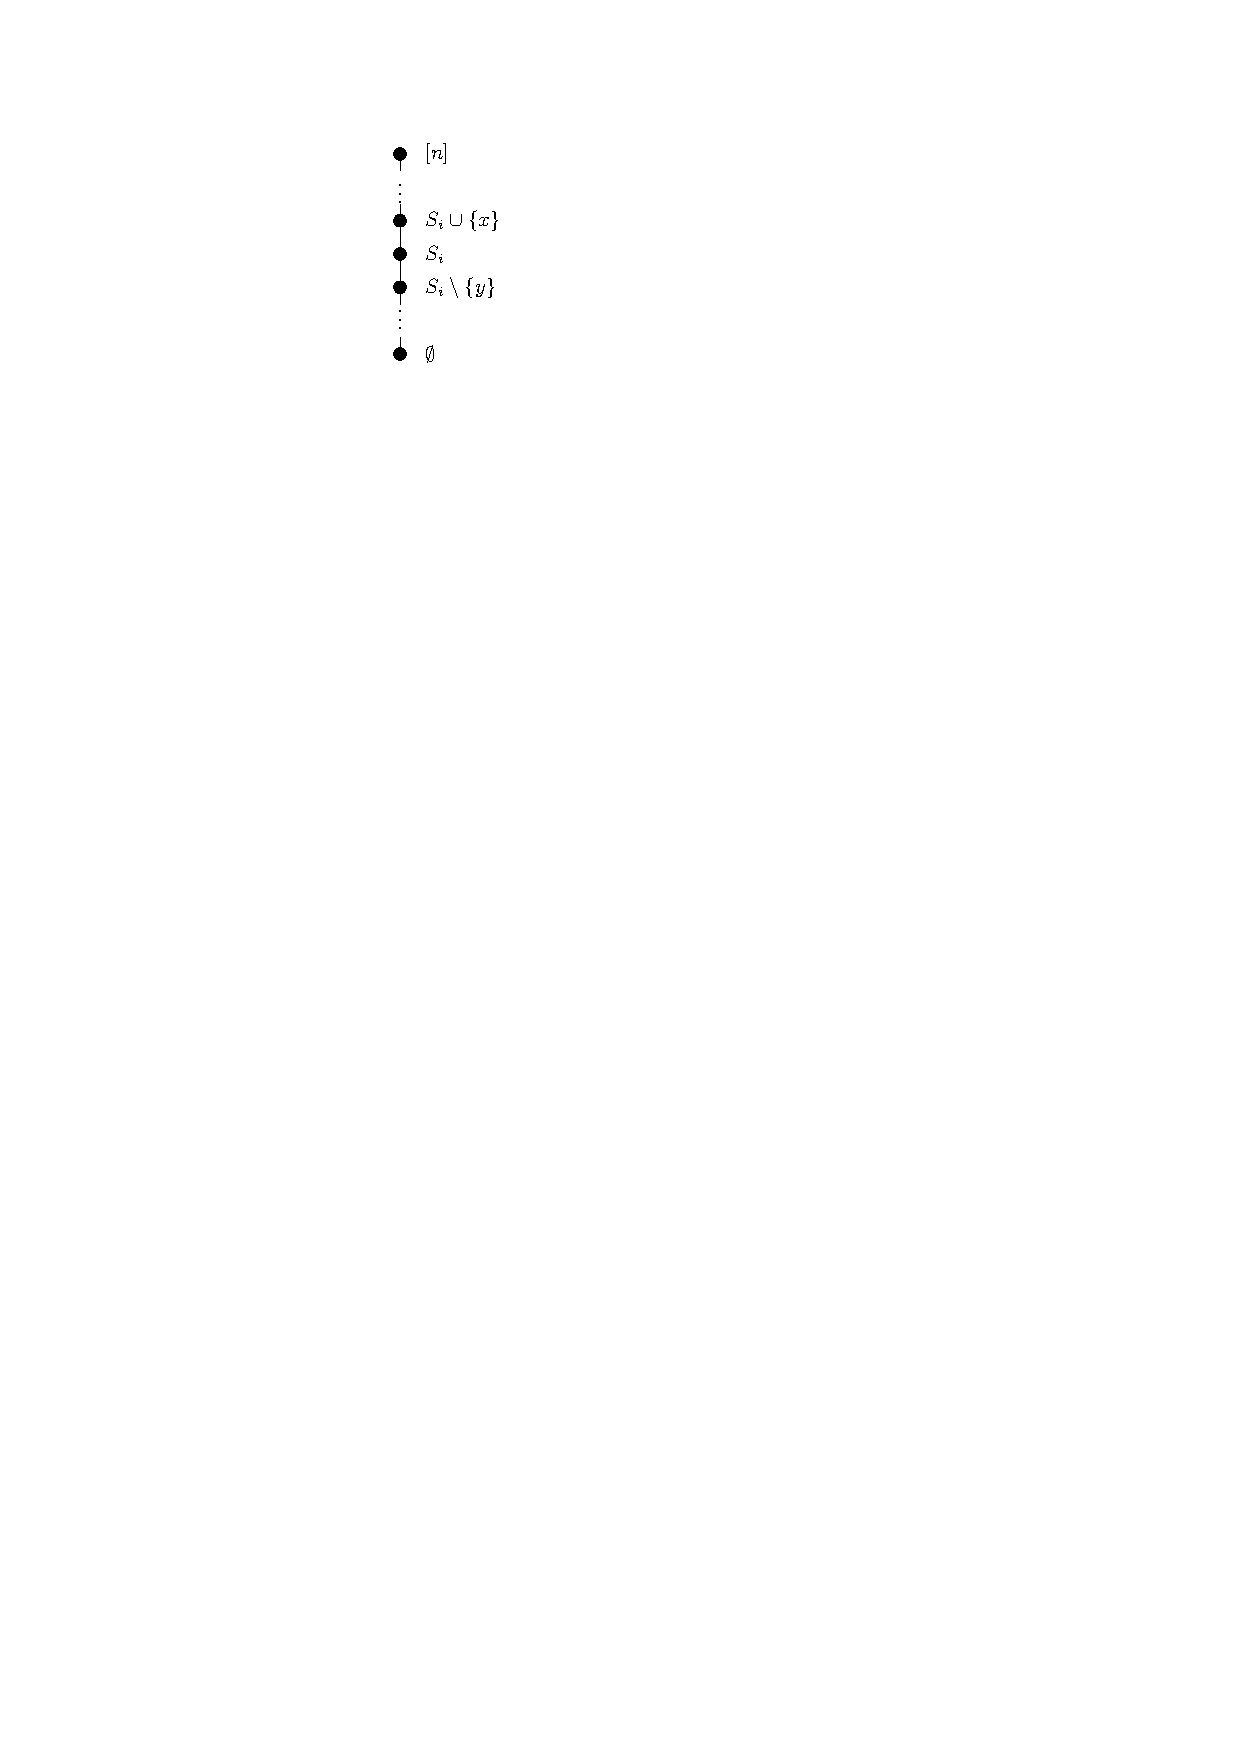
\includegraphics[width=0.1\linewidth]{figures/max-len-chain.pdf}
        \caption{Each subset must differ from the previous and next subset by exactly one element in a maximal chain. Otherwise, we form a chain of longer length by inserting a new subset in between.}
        \label{fig:max-len-chain}
    \end{figure}

    We also observe that there are exactly $n!$ many maximal chains, each corresponding to one ordering (permutation) to remove elements from $[n]$.

    For any $i \neq j$, $\mathcal{C}_i \cap \mathcal{C}_j = \emptyset$ because otherwise there would be a chain $C$ with $S_i,S_j \in C$ and hence $S_i$ and $S_j$ are comparable, which is a contradiction to our assumption that $S_i$ and $S_j$ are members of a maximal \textbf{antichain}. It follows that
    $$
    \left| \bigcup_{i=1}^w \mathcal{C}_i \right| = \sum_{i=1}^w |\mathcal{C}_i| \leq n!
    $$
    Since $|\mathcal{C}_i| = |S_i|! \cdot (k-|S_i|)!$, it follows that
    $$
    \sum_{i=1}^w |\mathcal{C}_i| = \sum_{i=1}^w (|S_i|! \cdot (k-|S_i|)!) \leq n!
    $$
    and hence
    $$
    \sum_{i=1}^w \frac{|S_i|! \cdot (k-|S_i|)!}{n!} = \sum_{i=1}^w \frac{1}{\binom{n}{|S_i|}} \leq 1
    $$
    by definition of combination. It follows from $\binom{n}{|S_i|} \leq \binom{n}{\floor{n/2}}$ that
    $$
    \sum_{i=1}^w \frac{1}{\binom{n}{\floor{n/2}}} \leq \sum_{i=1}^w \frac{1}{\binom{n}{|S_i|}}\leq 1
    $$
    and $w \leq \binom{n}{\floor{\frac{n}{2}}}$. Therefore, $\mathsf{width}(\mathbb{P}) \leq \binom{n}{\floor{\frac{n}{2}}}$ and because $\binom{n}{\floor{\frac{n}{2}}}$ is also a lower bound, $\mathsf{width}(\mathbb{P}) = \binom{n}{\floor{\frac{n}{2}}}$.
\end{proof}

\chapter{Dilworth's Theorem}
\section{Dilworth's Theorem}

\begin{theorem}[Dilworth's Theorem]
    Let $\mathbb{P} = (X,P)$ be a poset with width $w$. There is a partition of $X$ into $w$ chains $C_1,\ldots,C_w$. Moreover, this partition is optimal and it is not possible to cover $\mathbb{P}$ with fewer than $w$ chains.
\end{theorem}

There is also a dual version of Dilworth's theorem.

\begin{theorem}[Dilworth's Theorem (dual)]
    Let $\mathbb{P} = (X,P)$ be a poset with height $h$. There is a partition of $X$ into $h$ antichains $A_1,\ldots,A_h$. Moreover, this partition is optimal and it is not possible to cover $h$ with feweer than $h$ antichains.
\end{theorem}

Assuming the existence of such partition as described in Dilworth's theorem, we first prove optimality.

\begin{proof} (of optimality)
    \hfill

    Let $\mathbb{P} = (X,P)$ be a poset with width $w$. By way of contradiction, suppose that $X$ can be partitioned into $k$ disjoint chains $C_1,\ldots, C_k$ such that $k < w$. Take an antichaim $A$ of size $w$ and consider a map $f:\; A \to \{1,\ldots,k\}$ such that $f(x) = i \iff x \in C_i$ ($f$ outputs the index of the chain containing $x$). However, by Pigeonhole Principle, there is some $C_i$ containing at least two distinct members of $A$ and hence are comparable. This is a contradiction to the assertion that $A$ is an antichain.
\end{proof}

Next, we prove the existence of such optimal partition using induction on $|X|$.

\begin{proof} (of existence)
    \hfill

    \textbf{Base Case}: If $|X| = 1$, the poset contains exactly one element is the one point linear (total) order, so $X$ is a chain itself and we are done.

    \textbf{Inductive Step}: Take a poset $\mathbb{P} = (X,P)$ with width $w$ and height $h$. Assume that Dilworth's theorem holds for all posets with cardinality $k < |X|$.

    Let $C = \{x_1,\ldots,x_h\}$ be a maximal chain in $\mathbb{P}$ and consider the subposet $\mathbb{Q} = (X \setminus C,\, P \cap (X \setminus C)^2)$. Without loss of generality, suppose $x_1 <_{\mathbb{P}} <_{\mathbb{P}} \cdots <_{\mathbb{P}} x_h$. Note that $\mathsf{width}(\mathbb{Q}) \leq \mathsf{width}(\mathbb{P})$.

    Case 1: $\mathsf{width}(\mathbb{Q}) < \mathsf{width}(\mathbb{P})$. Then, $\mathsf{width}(\mathbb{Q}) = w-1$ because we only removed one chain to get from $\mathbb{P}$ to $\mathbb{Q}$ and if the width of $\mathbb{Q}$ is smaller than $w-1$, this would mean that some pair of elements in $C$ is not comparable, which would lead to a contradiction. Apply the induction hypothesis to $\mathbb{Q}$ to cover it with $w-1$ chains $C_1, \ldots, C_{w-1}$. Then, adding back $C$ gives us $C_1,\ldots,C_{w-1},C$, which is a cover of $\mathbb{P}$ with $w$ chains.

    Case 2: $\mathsf{width}(\mathbb{Q}) = \mathsf{width}(\mathbb{P})$. Then, there exists an antichain $A = \{a_1,\ldots,a_w\}$ of size $w$ in $\mathbb{Q}$. Let
    $$
    P^- = \{ x \in P \mid \exists i.\,x \leq_{\mathbb{P}} a_i \}
    $$
    $$
    P^+ = \{ x \in P \mid \exists i.\, x \geq_{\mathbb{P}} a_i \}
    $$
    Pictorially, $P^+$ is the set of all elements larger than some $a_i$ under $\leq_{\mathbb{P}}$ and $P^-$ is the set of all elements smaller than some $a_i$ under $\leq_{\mathbb{P}}$.

    \begin{figure}[htbp]
        \centering
        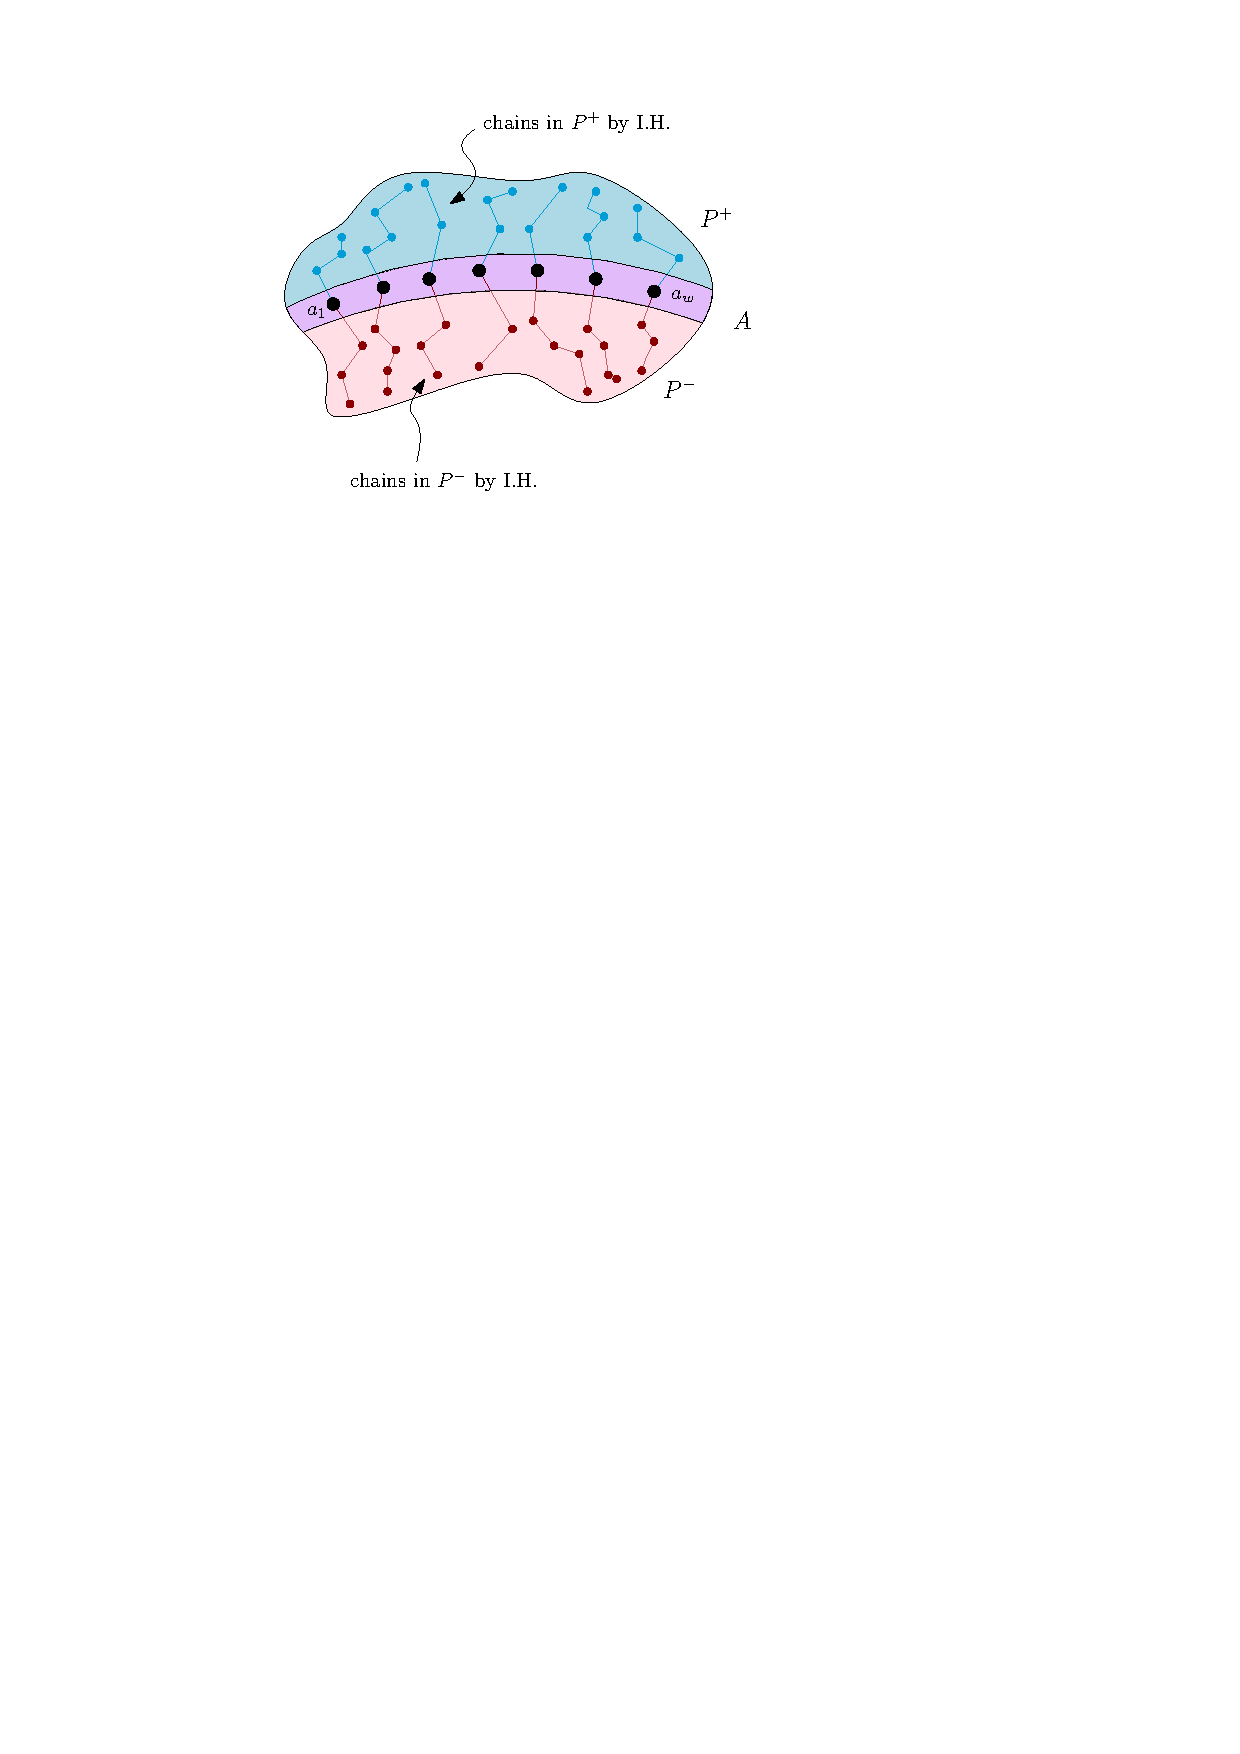
\includegraphics[width=0.4\linewidth]{figures/dilworth-proof-partition.pdf}
        \caption{We partition $P$ into $P^+$ and $P^-$ such that $P^+ \cap P^- = A$ and $P^+ \cup P^- = P$. Then, we take the $w$ chains in $P^+$ and concatenate with the $w$ chains in $P^-$ to form a set of $w$ disjoint chains in $P$.}
        \label{fig:dilworth-proof-partition}
    \end{figure}

    We note that
    \begin{enumerate}
        \item $P = P^- \cup P^+$. Otherwise, there would be an element $x \in P$ that is incomparable with every elements of $A$ and $A$ would not have been a max-size antichain.
        \item $P^- \cap P^+ = A$. Otherwise, there would exist $x,i,j$ such that $a_i <_{\mathbb{P}} x <_{\mathbb{P}} a_j$ so $A$ is not antichain.
        \item $x_h \not\in P^-$. Otherwise, $x <_{\mathbb{P}} a_i$ for some $i$ and the chain $C$ is not a maximal chain.
    \end{enumerate}

    By the third observation, $|P^-| < |P|$. Apply the inductive hypothesis, and we see that $P^-$ can be partitioned into $w$ chains $C^-_1,\ldots, C^-_w$. $a_i$ would be the \textbf{minimal element} in each $C^-_i$ because otherwise, $C^- \in P^- \cup P^+ \setminus A$, which contradicts the second observation. Using the same argument, we show that $P^+$ can be partitioned into $w$ chains $C^+_1,\ldots,C^+_w$ with $a_i$ as the minimal element of $C^+_i$.

    Now we construct the chains in $P$. Let $C_i = C^-_i \cup C^+_i$ so $P = \bigcup_{i=1}^w C_i$. From the second observation, it is clear that $C_i$ is a chain for $i = \{1,\ldots,w\}$.

    By induction, Dilworth's theorem holds for all posets.
\end{proof}

\section{Erd\"os-Szekeres's Theorem}

\begin{theorem}[Erd\"os-Szekeres]
    Let $\{x_i \mid i \in [rs + 1]\}$ be a family of $rs + 1$ distinct real numbers. There is a strictly increasing subsequence of length $r+1$ or a strictly decreasing subsequence of length $s+1$.
\end{theorem}

Erd\"os-Szekeres's theorem can be proved using the Pigeonhole Principle. Here, we consider an alternative proof using Dilworth's theorem.

\begin{proof}
    Consider the poset $\mathbb{P} = (X,P)$ where
    $$
    X = \{ (i,x_i) \mid i \in [rs + 1]\}
    $$
    and $(i,x_i) \leq_{\mathbb{P}} (j,x_j)$ if and only if $i \leq j$ and $x_i \leq x_j$.

    If $\mathsf{height}(\mathbb{P}) \geq r+1$, we are done since a maximal chain contains strictly increasing subsequence $x_{n_k}$ of size at least $r+1$. 
    
    Hence, suppose $\mathsf{height}(\mathbb{P}) \leq r$. By Dilworth's theorem, there exists a partition of $P$ into $w$ chains $C_1,\ldots,C_w$. Note that $|C_i| \leq r$, so $w \geq s + 1$. Otherwise, we can cover $X$ of size $rs + 1$ with $\bigcup_{i=1}^w C_i$ which has at most $rs$ points, which is a contradiction.

    It follows that there is an antichain $A = \{(n_1,x_{n_1}),\ldots,(n_{r+1}, x_{n_{r+1}})\}$ where we may assume that $i < j$ implies $n_i < n_j$. By the way we defined $\mathbb{P}$, if $n_i < n_j$, then $x_{n_i} > x_{n_j}$ or else $A$ would not be an antichain. It follows then that $x_{n_i}$ is a decreasing subsequence of size at least $s+1$.
\end{proof}

\section{Linear Extensions}

\begin{definition}[Linear Extension]
    Let $\mathbb{P} = (X,P)$ be a poset. A linear extension of $\mathbb{P}$ is a linear (total) order $\mathbb{L} = (X,L)$ where $P \subseteq L$ (such that for all $a,b \in X$, $a \leq_{\mathbb{P}} b \iff a \leq_{\mathbb{L}} b$).
\end{definition}

Questions pertaining to extending posets to linear (total) orders relate to sorting algorithms. The following theorem states that every poset has a linear extension.

\begin{theorem}
    Let $\mathbb{P} = (X,P)$ be a poset. There is a linear extension $\mathbb{L} = (X,L)$ of $\mathbb{P}$.
\end{theorem}

\begin{proof}
    We prove this by recursively creating a sequence of extensions $\mathbb{P}_i = (X,P_i)$ of $\mathbb{P}$ starting from $\mathbb{P}$, and in the end we get a linear order.

    For some index $i$, we have a poset $\mathbb{P}_i$. If $\mathbb{P}_i$ is not a linear order, there must be two points $a,b \in X$ that are not $\mathbb{P}_i$-comparable. We construct $\mathbb{P}_{i+1}$ to be $(X,P_{i+1})$ where $P_{i+1}$ is
    $$
    P_{i+1} = P_i \cup \{ (a,b) \} \cup \{ (x,y) \in X^2 \mid x \leq_{\mathbb{P}_i} a \land b \leq_{\mathbb{P}_i} y \}.
    $$
    One can verify that $\mathbb{P}_{i+1}$ satisfies all the required properties of a poset, in particular, transitivity.

    We perform this process starting from the original poset $\mathbb{P}$ and eventually the process must half. Otherwise, we would have an infinite sequence of pairs $(a_i,b_i) \in X^2$ that are incomparable, contradicting that $X$ is finite.
\end{proof}

\part{Inclusion-Exclusion}

\chapter{Inclusion-Exclusion Principle}
\section{Inclusion-Exclusion Principle}

\begin{definition} \label{def:inc-exc-notation}
    Let $S$ be a set. Fix a collection $A_i \subseteq S$ indexed by $i \in \{1,\ldots,n\}$. Given $I \subseteq \{1,\ldots,n\}$, we let $A_I = \bigcap_{i\in I} A_i$. In particular, we set $A_{\emptyset} = S$.
\end{definition}

In simple terms, $x \in A_I$ if and only if $\forall i \in I.\, x \in A_i$.

As an example, consider $S = \{1,\ldots,20\}$ and $A_1 = \{ x \in S \mid \text{$x$ is divisible by 2 }\}$, $A_2 = \{ x \in S \mid \text{$x$ is divisible by 3 }\}$, and $A_3 = \{ x \in S \mid \text{$x$ is divisible by 4}\}$. Then, we have:
\begin{itemize}
    \item $A_{\emptyset} = S$
    \item $A_{\{1,2\}} = \{6,12,18\}$
    \item $A_{\{1,3\}} = \{8, 16\}$
    \item $A_{\{1,2,3\}} = \{\}$  
\end{itemize}

We are all familiar with the addition principle: given two disjoint sets $A, B$ such that $A \cap B = \emptyset$,
$$
|A \cup B| = |A| + |B|
$$
In the case where $A$ and $B$ are not disjoint, we can simply remove the count for the common elements among $A$ and $B$ that were double-counted.
$$
|A \cup B| = |A| + |B| - |A \cap B|
$$
We further observe that four three sets $A,B,C$, we have
$$
|A \cup B \cup C| = |A| + |B| + |C| - |A \cap B| - |A \cap C| - |B \cap C| - |A \cap B \cap C|
$$
The generalization of this is called the Inclusion-Exclusion Principle. There are multiple equivalent formulations of the Inclusion-Exclusion Principle.

\begin{theorem}[Inclusion-Exclusion Principle]
    Let $S$ be a set. Let $A_1,\ldots,A_n \subseteq S$ be subsets of $S$ indexed by $i \in \{1,\ldots,n\}$. Then, the number of elements in $S$ that is in none of $A_i$ is
    $$
    \left| \bigcap_{i=1}^n \overline{A_i} \right| = \left| S \setminus \bigcup_{i = 1}^n A_i \right| = \sum_{I \subseteq [n]} (-1)^{|I|} |A_I|
    $$
    and equivalently,
    $$
    \left| \bigcup_{i=1}^n A_i \right| = \sum_{\substack{I \subseteq [n] \\ I \neq \emptyset}} (-1)^{|I|+1} |A_I|
    $$
\end{theorem}

If stated without using the notation introduced in Definition \ref{def:inc-exc-notation}, the Inclusion-Exclusion Principle can be stated as follows.

\begin{theorem}
    If $A_i \subseteq X$ for $1 \leq i \leq n$, then
    $$
    \left| \bigcup_{i=1}^n A_i \right| = \sum_{k=1}^n \left( (-1)^{k+1} \sum_{\{i_1,\ldots,i_k\} \subseteq [n]} \left| \bigcap_{j=1}^k A_{i_j} \right| \right)
    $$
    and equivalently
    $$
    \left| \bigcap_{i=1}^n \overline{A_i} \right| = |X| + \sum_{k=1}^n \left( (-1)^{k} \sum_{\{i_1,\ldots,i_k\} \subseteq [n]} \left| \bigcap_{j=1}^k A_{i_j} \right| \right)
    $$
\end{theorem}

We give a proof of the Inclusion-Exclusion Principle using induction.

\begin{proof}
    \hfill

    Base Case: $n = 1$. $A_1$ is the only subset of $S$ in the collection. $| \bigcup_{i=1}^n \overline{A_i}| = |S| - |A_i| = \sum_{I \in [1]} (-1)^{|I|} |A_I|$.

    Inductive Step: Let $n \in \N$ be arbitrary. Assume that the principle holds for all $k \leq n$. Consider a collection of subsets $A_1,\ldots,A_{n+1} \subseteq S$. Let $B_i = A_i \cap A_{n+1}$ for $i \in \{1,\ldots,n\}$. Let $B_I = A_{n+1} \cap \bigcap_{i \in I}A_i$. Note that $B_{\emptyset} = A_{n+1}$.

    We know by induction hypothesis that
    $$
    \left| S \setminus \bigcup_{i=1}^n A_i \right| = \sum_{I \subseteq [n]} (-1)^{|I|} |A_I| \qquad \left| A_{n+1} \setminus \bigcup_{i=1}^n A_i \right| = \sum_{I \subseteq [n]} (-1)^{|I|} |B_I|
    $$
    In other words, $\sum_{I \subseteq [n]} (-1)^{|I|} |A_I|$ counts the number of elements in $S$ that is not in $A_1,\ldots,A_n$. Similarly, $\sum_{I \subseteq [n]} (-1)^{|I|} |B_I|$ counts the number of elements in $S$ that satisfied only $A_{n+1}$. Now, consider
    $$
    \begin{aligned}
        \sum_{I \subseteq [n+1]} (-1)^{|I|} |A_I| &= \sum_{I \subseteq [n]} (-1)^{|I|} |A_I| + \sum_{I \subseteq [n]} (-1)^{|I| + 1} |A_{I \cup \{n+1\}}| \\
        &= \sum_{I \subseteq [n]} (-1)^{|I|} |A_I| - \sum_{I \subseteq [n]} (-1)^{|I|} |A_{I \cup \{n+1\}}| & \text{take out $-1$} \\
        &= \left| S \setminus \bigcup_{i=1}^n A_i \right| - \sum_{I \subseteq [n]} (-1)^{|I|} |A_{I \cup \{n+1\}}| & \text{by I.H.} \\
        &= \left| S \setminus \bigcup_{i=1}^n A_i \right| - \sum_{I \subseteq [n]} (-1)^{|I|} |B_I| & \text{by definition of $B_I$} \\
        &= \left| S \setminus \bigcup_{i=1}^n A_i \right| - \left| A_{n+1} \setminus \bigcup_{i=1}^n A_i \right| & \text{by I.H.} \\
        &= \left| S \setminus \bigcup_{i=1}^{n+1} A_i \right|
    \end{aligned}
    $$
\end{proof}

Let's consider the following example.

\begin{example}
    Count the number of integer solutions to the equation $x_1 + x_2 + x_3 + x_4 = 100$ with $x_1, x_2 \leq 10$ and $x_i \geq 0$ for all $i \in \{1,2,3,4\}$.

    Let $S$ be the set of solutions with $x_i \geq 0$ for all $i \in \{1,2,3,4\}$. Let $A_1$ be the set of solutions with $x_1 \geq 10$ and $x_i \geq 0$ for all $i \in \{1,2,3,4\}$. Let $A_2$ be the set of solutions with $x_2 \geq 10$ and $x_i \geq 0$ for all $i \in \{1,2,3,4\}$.

    Notice that the quantity that we want to count is equal to $|S \setminus (A_1 \cup A_2)|$. If a solution in $S$ fails any of our conditions, it must be in either $A_1$ or $A_2$. We can count $|S|$ using the stars-and-bars technique (since we are essentially trying to partition 100 elements into 4 groups by placing 3 bars). So it follows that we have $|S| = \binom{100+3}{3}$. We can do the same to count $|A_1|$ and $|A_2|$. It follows from the Principle of Inclusion-Exclusion that
    $$
    \begin{aligned}
        |S \setminus (A_1 \cup A_2)| &= |S| - (|A_1|+|A_2|) + |A_1 \cap A_2| \\
        &= \binom{100+3}{3} - \left( \binom{90+3}{3} + \binom{90+3}{3} \right) - \binom{80 + 3}{3}
    \end{aligned}
    $$
\end{example}

\section{Counting Surjections}

Recall that a function $f:\; X \to Y$ is a surjection if for all $y \in Y$, there exists an $x \in X$ such that $f(x) = y$. Also, the number of functions from $X$ to $Y$ is $|Y|^{|X|}$.

\begin{theorem}
    Let $S(n,m)$ be the number of surjections $f:\; [n] \to [m]$. Then,
    $$
    S(n,m) = \sum_{k=0}^m (-1)^k \binom{m}{k} (m-k)^n
    $$
\end{theorem}

\begin{proof}
    Let $F$ be the set of all functions from $[n]$ to $[m]$. For each $i \in [m]$, let
    $$
    A_i = \{f \in F \mid \forall x \in [n].\, f(x) \neq i \}.
    $$
    We note that $F \setminus \bigcup_{i = 1}^m A_i$ contains all surjective functions because we have removed all the non-surjective functions. For any $I \subseteq [m]$ of size $k$, $|A_I| = (m-k)^n$. This is because each $A_i$  It follows that
    $$
    \begin{aligned}
        S(n,m) &= \left| F \setminus \bigcup_{i=1}^m A_i \right| \\
        &= \sum_{I \subseteq [m]} (-1)^{|I|} |A_I| \\
        &= \sum_{k=0}^m \sum_{\substack{I \subseteq [m] \\ |I| = k}} (-1)^{I} |A_I| \\
        &= \sum_{k=0}^m \sum_{\substack{I \subseteq [m] \\ |I| = k}} (-1)^{I} (m-k)^n
    \end{aligned}
    $$
    Note that there are $\binom{m}{k}$ ways to choose a subset of size $k$ from a set of size $m$. Hence,
    $$
    S(n,m) = \sum_{k=0}^m \sum_{\substack{I \subseteq [m] \\ |I| = k}} (-1)^{I} (m-k)^n = \sum_{k=0}^m \binom{m}{k} (-1)^{I} (m-k)^n
    $$
\end{proof}

\chapter{More Applications of Inclusion-Exclusion}
\section{Derangement}

\begin{definition}[Derangement]
    A derangement is a permutation $s:\; [n] \to [n]$ with the property that for all $i \in [n].\; s(i) \neq i$ We denote the number of derangements with the reverse factorial (or the subfactorial or $n$th derangement number), $d_n$ or $!n$.
\end{definition}

Note that $d_n < n!$. In other words, a derangement is a permutation with no fixed point. This interpretation gives us some hints on how to count derangements, which is formalized by the following theorem.

\begin{theorem}
    $$
    d_n = \sum_{k=0}^n (-1)^k \binom{n}{k} (n-k)! = n! \sum_{k=0}^n \frac{(-1)^k}{k!}
    $$
\end{theorem}

\begin{proof}
    For $i \in [n]$, let $A_i$ be the set of permutations $s$ such that $s(i) = i$ (the permutations that violates the definition of a derangement due to a fixed point at the $i$th value).

    Let $S$ be the set of all permutations of $[n]$. Then, the number of derangements is
    $$
    S \setminus \bigcup_{i \in [n]} A_i
    $$
    For any $I \subseteq [n]$ of size $k$, $|A_I| = (n-k)!$. This is from the observation that the positions in $I$ are not changed in the permutation so only $(n-k)$ elements are permuted. Then, we have
    $$
    \begin{aligned}
        d_n &= \left| S \setminus \bigcup_{i \in [n]} A_i \right| \\
        &= \sum_{I \subseteq [n]} (-1)^{|I|} |A_I| \\
        &= \sum_{k=0}^n (-1)^k \binom{n}{k} (n-k)!
    \end{aligned}
    $$
\end{proof}

\section{Number Theory}

\begin{definition}[Greatest Common Divisor]
    Let $a,b \in \Z$. The \textit{\textbf{greatest common divisor}} of $a$ and $b$ is the largest of all common divisors of $a$ and $b$. The notation for the GCD of $a$ and $b$ is $(a,b)$ or $\gcd(a,b)$.
\end{definition}

We say two integers $n,m$ are \textbf{relatively prime} if $\gcd(n,m)=1$. In other words, $n$ and $m$ are relatively prime if and only if they share no prime divisors.

\begin{definition}[Euler's Totient Function]
    For $n \in \N$, we let
    $$
    \phi(n) = | \{m \in [n] \mid \gcd(m,n) = 1\}
    $$
    known as the Euler's phi or \textbf{Euler's totient function}.
\end{definition}

Euler's totient function counts the positive integers up to a given integer $n$ that are relatively prime to $n$. The Euler's totient function is of great interest in the field of number theory and group theory. We will derive a closed form formula for $\phi(n)$ using combinatorics, but before we do that, we will first prove a lemma regarding prime divisibility.

\begin{lemma}
    Let $n \geq 2$ be an integer, and let $p_1,\ldots,p_k$ be a collection of distinct primes that divide $n$. Then, there are $\frac{n}{p_1\cdots p_k}$ integers in $\{1,\ldots,n\}$ that are divisible by $p_1,\ldots,p_k$.
\end{lemma}

\begin{proof}
    Let $m \in \N$ where $m \leq n$. Suppose that $m$ is divisible by all $p_1,\ldots,p_k$. It follows from the Fundamental Theorem of Arithmetics that $m = p_1 \cdots p_k \cdot \alpha$ for some $\alpha \in \N$. Hence, $p_1 \cdots p_k \leq p_1 \cdots p_k \cdot \alpha \leq n$. It follows that $1 \leq \alpha \leq \frac{n}{p_1 \cdots p_k}$. Since $\frac{p}{p_1\cdots p_k}$ is an integer, the set $\{ \alpha \cdot p_1 \cdots p_k \mid \alpha \in \{1,\ldots,\frac{n}{p_1\cdots p_k}\}\}$ contains all the positive integers divisible by all of $p_1,\ldots,p_k$. The size of the set is $\frac{n}{p_1\cdots p_k}$.
\end{proof}

Now we are ready to derive a closed form formula for $\phi(n)$ using Inclusion-Exclusion.

\begin{theorem}
    For all $n \geq 2$, if $p_1,\ldots,p_k$ are all the prime factors of $n$, then
    $$
    \phi(n) = n \prod_{i=1}^k \frac{p_i - 1}{p_i}
    $$
\end{theorem}

\begin{proof}
    For each $i \in \{1,\ldots,k\}$, let $A_i$ be the set of integers in $\{1,\ldots,n\}$ that are divisible by $p_i$. Note that $[n] \setminus \bigcup_{i=1}^k A_i$ is the set of positive integers less than or equal to $n$ that are relatively prime with $n$. By the previous lemma, for all $I \subseteq \{1,\ldots,n\}$, $|A_I| = n \prod_{i \in I} 1/p_i$.

    Then,
    $$
    \begin{aligned}
        \phi(n) &= \sum_{I \subseteq [k]} (-1)^{|I|} \cdot n \cdot \prod_{i \in I} \frac{1}{p_i} \\
        &= n \sum_{I \subseteq [k]} (-1)^{|I|} \prod_{i \in I} \frac{1}{p_i} \\
        &= n \sum_{I \subseteq [k]} \prod_{i \in I} \frac{(-1)}{p_i} \\
        &= n \prod_{i=1}^k \left( 1 - \frac{1}{p_i} \right) \\
        &= n \prod_{i=1}^k \frac{p_i - 1}{p_i}
    \end{aligned}
    $$
\end{proof}

\part{Combinatorial Game Theory}

\backmatter

\bibliographystyle{abbrvnat}
\bibliography{stringbook}
\addcontentsline{toc}{chapter}{Bibliography}

\printindex

\end{document}

